\documentclass[12pt,a4paper]{report}
%% does not work in Latex2Html mode
%\usepackage{hyperref}
\usepackage{url}
\usepackage{html}
\usepackage{epic}
\usepackage{eepic}
\usepackage{makeidx}
\usepackage{array}
\usepackage{times}
\usepackage{amsmath}
\usepackage[dvips]{epsfig,rotating}
\usepackage{dingbat}
\usepackage{listings}
\usepackage{graphicx}

\lstnewenvironment{code}[1][]
{\textbf{Code Listing} \hspace{1cm} \hrulefill \lstset{language=C++, basicstyle=\ttfamily\scriptsize}}
{\hrule\smallskip}
%{\textbf{Code Listing} \hspace{1cm} \hrulefill \lstset{language=C++, basicstyle=\ttfamily\scriptsize, #1}}

\lstnewenvironment{codeln}[1][]
{\textbf{Code Listing} \hspace{1cm} \hrulefill \lstset{language=C++, basicstyle=\ttfamily\scriptsize, numbers=left, numberstyle=\tiny, stepnumber=1, numbersep=5pt}}
{\hrule\smallskip}

\lstnewenvironment{smallcode}[1][]
{\lstset{language=C++, basicstyle=\ttfamily\scriptsize}}
{\smallskip}

\usepackage{pdfdraftcopy}             % Draft
\draftstring{V1.0 Draft}
%% Define a new 'leo' style for the package that will use a smaller font.
%\makeatletter
%\def\url@leostyle{%
 % \@ifundefined{selectfont}{\def\UrlFont{\sf}}{\def\UrlFont{\small\ttfamily}}}
%\makeatother
%% Now actually use the newly defined style.
%\urlstyle{leo}

\setlength\topmargin{0.0cm}
%\setlength\oddsidemargin{3.501cm}
%\setlength\evensidemargin{3.501cm}
\renewcommand{\arraystretch}{1.5}


% Definition neuer Zeichen
\newcommand{\R}{{\mathbb R}}
\newcommand{\N}{{\mathbb N}}
\newcommand{\Z}{{\mathbb Z}}
% Standard Notationen
\newcommand{\vc}[1]{\mbox{\boldmath $#1$}}
\newcommand{\sv}[1]{\mbox{\boldmath $\vec{#1}$}}
\newcommand{\mx}[1]{\mbox{\boldmath $\underline{#1}$}}
\newcommand{\op}[1]{\mathcal{#1}}
% Sonstige Abkuerzungen
\newcommand{\backpar}{\rule{1mm}{0mm}\\[-5ex]\rule{1mm}{0mm}}
\newcommand{\ds}{\displaystyle}
\newcommand{\AND}{\quad\mbox{and}\quad}
\newcommand{\diag}{\mbox{diag }}
\newcommand{\arrstr}[1]{\rule[0mm]{0mm}{#1}}
\newcommand{\hstrut}[1]{\rule{0mm}{#1}}
\newlength{\mylablen}
\newlength{\mycaplen}
\newlength{\myislen}
% caption fuer Bilder
\newcommand{\fcap}[2]{\refstepcounter{figure} \settowidth{\mycaplen}{#2}
\settowidth{\mylablen}{\bf Figure \thefigure:~}
\settowidth{\myislen}{\textwidth-\mylablen}
\begin{center}
{\bf Figure \thefigure:~}\ifthenelse{\mycaplen > \myislen}{\parbox[t]{\textwidth-\mylablen}{#2}\label{#1}}{#2\label{#1}}\end{center}}
% caption fuer Tabellen
\newcommand{\tcap}[2]{\refstepcounter{table} \settowidth{\mycaplen}{#2}
\settowidth{\mylablen}{\bf Table \thetable:~}
\settowidth{\myislen}{\textwidth-\mylablen}
\begin{center}
{\bf Table \thetable:~}\ifthenelse{\mycaplen > \myislen}{\parbox[t]{\textwidth-\mylablen}{#2}\label{#1}}{#2\label{#1}}\end{center}}
%
\newtheorem{theorem}{Theorem}
\newtheorem{lemma}{Lemma}
\newtheorem{corollary}{Corollary}
\newtheorem{remark}{Remark}
\newtheorem{definition}{Definition}
\newtheorem{proposition}{Proposition}
\newenvironment{proof}{{\bf Proof:}}{{}\hfill{$\square$}\par\smallskip}

\renewcommand{\topfraction}{0.9}
\renewcommand{\bottomfraction}{0.9}
\renewcommand{\textfraction}{0.1}

\newcommand{\ipplversion}{\text{1.0 }}
\newcommand{\mad}{\textsc{mad }}
\newcommand{\madnine}{\textsc{mad9 }}
\newcommand{\madninep}{\textsc{mad9p }}
\newcommand{\madeight}{\textsc{mad8 }}
\newcommand{\pooma}{\textsc{pooma }}
\newcommand{\classic}{\textsc{classic }}

\newcommand{\ippl}{\textsc{I$\text{P}^2$L }}


\newcommand{\opal}{\textsc{OPAL }}
\newcommand{\opalt}{\textsc{OPAL-t }}
\newcommand{\opalcycl}{\textsc{OPAL-cycl }}
\newcommand{\opalmap}{\textsc{OPAL-map }}

\newcommand{\partroot}{\textsc{H5PartROOT }}

\newcommand{\lieop}[1]
{{:}{#1}{:}}
\renewcommand{\arraystretch}{2.0}

\newcommand{\rms}[1]
{\overset{\sim}{#1}}

% Pfister stuff
\def\C{{{{\rm {\mbox{\small l}}} \kern -.50em {\rm C}}}}
\def\R{{{{\rm l} \kern -.15em {\rm R}}}}
\def\N{{{{\rm l} \kern -.15em {\rm N}}}}
\def\E{{{{\rm l} \kern -.15em {\rm E}}}}
\def\P{{{{\rm l} \kern -.15em {\rm P}}}}
\def\D{{{{\rm l} \kern -.15em {\rm D}}}}
\def\L{{{{\rm l} \kern -.15em {\rm L}}}}
\def\Z{{{{\rm Z} \kern -.35em {\rm Z}}}}
\def\Q{{{{\rm {\mbox{\small l}}} \kern -.45em {\rm Q}}}}
\def\qQ{{{{\rm {\mbox{\scriptsize l}}} \kern -.33em {\rm Q}}}}
\def\v{\vspace{1ex}}
\def\-v{\vspace{-1ex}}
\def\vv{\vspace{2ex}}
\def\vvv{\vspace{3ex}}
\def\vn{\vspace{3ex}\noindent}
\def\hs{\hspace{-1ex}}
\def\n{\noindent}
\def\dsl{\dis\sum\limits}
\def\dis{\displaystyle}
\def\O{\Omega}
\def\o{\omega}
\def\fr{\mbox{\footnotesize $\dis\frac{1}{2}$}}
\def\frvier{\mbox{\footnotesize $\dis\frac{1}{4}$}}
\def\ov{\overline}
\def\b{\big[}
\def\B{\big]}
\def\i{\big\{}
\def\g{\big\}}
\def\e{\epsilon}
\def\f{\footnotesize}
\def\l{\ell^\prime}
\def\ll{\ell,\ell^\prime}
\def\r{\rightarrow}
\def\point{{\mbox{\large $.$}}}
\def\wl{\widetilde{\ell}}
\def\wll{\widetilde{\ell},\widetilde{\ell}^\prime}
\def\w{\widetilde}
\def\wh{\widehat}
\def\wt{\widetilde}
\def\cA{{\cal A}}
\def\cT{{\cal T}}
\def\cE{{\cal E}}
\def\oS{\overline{S}}
\def\oT{\overline{T}}
\def\cI{{\cal I}}
\def\cK{{\cal K}}
\def\cH{{\cal H}}
\def\cP{{\cal P}}
\def\cF{{\cal F}}
\def\cS{{\cal S}}
\def\cG{{\cal G}}
\def\cO{{\cal O}}
\def\cU{{\cal U}}

%% REAL ADA STUFF
\def\bx{{\bf x}}
\def\br{{\bf r}}
\def\bv{{\bf v}}
\newcommand{\matr}[1]{\mathcal{#1}}
 \newcommand{\myvec}[1]{\bf{#1}}
%\newcommand{\figref}[2]{#1 (see~Figure~\ref{fig:#2})}
%\newcommand{\tabref}[2]{#1 (see~Table~\ref{tab:#2})}
%\newcommand{\secref}[2]{#1 (see~Section~\ref{sec:#2})}
\newcommand{\mytabline}[2]{\texttt{#1} & #2 \\}
\renewcommand{\vec}{\myvec}

\makeindex

\renewcommand{\topfraction}{1.0}
\renewcommand{\bottomfraction}{1.0}
\renewcommand{\textfraction}{0.0}

\newenvironment{tex2html_nowrap}{}{}

\newcommand{\bibref}[2]{\hypercite{#1}{}{}{bib:#2}}

\newcommand{\tabline}[3]{\hyperref{\texttt{#1}}%
  {\texttt{#1} (}{)}{sec:#3} & #2 \\}
\newcommand{\figref}[2]{\hyperref{#1}{#1 (see~Figure~}{)}{fig:#2}}
\newcommand{\secref}[2]{\hyperref{#1}{#1 (see~Section~}{)}{sec:#2}}
\newcommand{\tabref}[2]{\hyperref{#1}{#1 (see~Table~}{)}{tab:#2}}
\begin{htmlonly}
\bodytext{bgcolor = "#ffffff"}
\end{htmlonly}

%\newcommand{\documentlabel}{ }

\begin{document}

\begin{titlepage}

\begin{htmlonly}
\begin{rawhtml}
<center>
PAUL SCHERRER INSTITUT
<br>
<h1>The IPPL Framework , Version 1.0</h1>
<h2>(Independent Parallel Particle Layer)</h2>
<h2>User's Reference Manual</h2>
<br>
Andreas Adelmann  
</center>
\end{rawhtml}
\end{htmlonly}

\begin{latexonly}
\begin{center}\normalsize

\includegraphics[width=1.\linewidth,angle=0]{figures/psi_logo_wide}
\end{center}
\vskip 0.7cm
PSI-PR-09-05
\begin{flushright}
%\documentlabel \\                    % document label
\end{flushright}
%\vskip 2.3cm
\begin{center}\LARGE                 % document title
{\bf The \ippl Framework} \\
(Independent Parallel Particle Layer) \\
Version \ipplversion \footnote{Release Date: \today} \\
{\bf User's Reference Manual}
\end{center}
\vskip 1.5em
\begin{center}                       % author
Andreas Adelmann, Yves Ineichen 
\vskip 2em
{\large Abstract}
\end{center}
\end{latexonly}
\begin{quotation}
 \ippl (Independent Parallel Particle Layer) is an object-oriented framework for particle based applications in computational science 
requiring high-performance parallel computers. One of \ippl 's most attractive features is its high performance on both single-processor and  distributed-memory multicomputers machines. As future releases of the library will also support shared-memory multicomputers, \ippl 's authors have had to think very carefully about how to obtain the best possible performance across a wide range of applications on different architectures.
\ippl  is a library of C++ classes designed to represent common abstractions in applications where {\em particles, fields} and operators like {\em FFT's} are needed.

Application programmers use and derive from these classes, which present a data-parallel programming interface at the highest abstraction layer.

Lower, to the user (programmer) hidden implementation layers encapsulate distribution and communication of data among processors. The supported platforms are: Linux based Beowulf clusters, Cray XT5/6, SGI Ultrix and the IBM Blue Gene series.

The main goals of the \ippl  framework includes:
\begin{itemize}
    \item Portability across serial, distributed, and parallel architectures with no change to source code
    \item Development of reusable, cross-problem-domain components to enable rapid application development
    \item High efficiency for kernels and components relevant to scientific simulation
    \item Framework design and development driven by applications from a diverse set of scientific problem domains
    \item Shorter time from problem inception to working parallel simulations 
\end{itemize}
 \ippl is currently in development the version here is the first "developer release". \ippl is inspired and partially based on POOMA r1 designed and implemented by scientists working at the Los Alamos National Laboratory's Advanced Computing Laboratory. 
 %Although \ippl  has received numerous additions the most importand are: 
%Fully ANSI C++ compatible, full 64Bit, HDF5 support and a Trilinos interface.

The report is organized as follow: in chapter 1 an introduction based on examples including installation instructions is presented. Chapter 2 and 3 are describing support classes followed by an discussion
on 3D parallel FFT's in \ippl. The next two chapters explaining the use of particles and fields. Appendix A - F describing design and implementation details of the most important classes in the
framework.
\end{quotation}
\vfill


\end{titlepage}

\tableofcontents
\listoftables
\listoffigures
\chapter{Introduction}
\label{sec:Introduction}
One of \ippl 's most attractive features is its high performance on both single-processor and distributed-memory multiprocessor machines. As future releases of the library will also support shared-memory machines. 

The heart of the problem \ippl 's authors face is that while data-parallel programming is a natural way to express many scientific and numerical algorithms, straightforward implementations of it do exactly the wrong thing on modern architectures, whose performance depends critically on the re-use of data loaded into cache. If a program evaluates A+B+C for three arrays A, B, and C by adding A to B, then adding C to that calculation's result, performance suffers both because of the overhead of executing two loops instead of one, but also (and more importantly) because every value in the temporary array that stores the result of A+B has to be accessed twice: once to write it, and once to read it back in. As soon as this array is too large to fit into cache, the program's performance will drop dramatically.

%The first section of this tutorial explains what \ippl  does to solve this problem. Subsequent sections discuss other advanced aspects of \ippl , such as how to build pointwise functions, or reduction functions that will execute efficiently regardless of how arrays are laid out in memory.

%\ippl  tries to resolve the tension between how programmers want to express their ideas, and what runs most efficiently on modern architectures, by delaying the evaluation of expressions until enough is known about their context to ensure that they can be evaluated efficiently. It does this by blocking calculations into units called iterates, and putting those iterates into a queue of work that is still to be done. Each iterate is a portion of a computation, over a portion of a domain. \ippl  tracks data dependencies between iterates dynamically to ensure that out-of-order computation cannot occur.

%Depending on the switches specified during configuration when the library is installed, and the version of the \ippl  library that a program is linked against, \ippl  will run in one of four different modes. In the first mode, the work queue doesn't actually exist. Instead, the single thread of execution in the program evaluates iterates as soon as they are "enqueued", i.e. work is done immediately. The result is that all of the calculations in a statement are completed by the time execution reaches the semi-colon at the end of that statement.

%In its second mode, \ippl  maintains the work queue, but all work is done by a single thread. The queue is used because the explicit parceling up of work into iterates gives \ippl  an opportunity to re-order or combine those iterates. While the overhead of maintaining and inspecting the work queue can slow down operations on small arrays, it makes operations on large arrays much faster.

%For example, consider the four function calls that perform red/black relaxation in the second tutorial. In order to get the highest possible performance out of the cache, all four of these expressions should be evaluated on a given cache block before any of the expressions are evaluated for the next cache block. Managing this by hand is a nightmare, both because cache size varies from machine to machine (even when those machines come from the same manufacturer), and because very slight changes in the dimensions of arrays can tip them in or out of cache. \ippl 's array classes and overloaded operators do part of the job by creating appropriately-sized iterates; its work queue does the rest of the job by deciding how best to evaluate them. The net result is higher performance for less programmer effort.

%\ippl 's third and fourth modes of operation are multi-threaded. Each thread in a pool takes iterates from the work queue when and as they become available. Iterates are evaluated independently; the difference between the two modes is that one is synchronous, and blocks after evaluating each data-parallel statement, while the other is asynchronous, i.e. permits out-of-order execution. The table below summarizes these four modes, along with the configuration arguments used to produce each.


\section{Example 1 Laplace solver using Jacobi iteration}
\begin{code}[caption={Laplace solver}]
#include "Ippl.h"
int main(int argc, char *argv[])
{
    Ippl ippl(argc,argv);
    Inform msg(argv[0]);
    const unsigned N=8;
    const unsigned Dim=2;

    Index IGLOBAL(N);  // Specify the global domain 
    Index JGLOBAL(N); 

    Index I(1, N-1); // Specify the interior domain
    Index J(1, N-1);
    FieldLayout<Dim> layout(IGLOBAL,JGLOBAL);
    GuardCellSizes<Dim> gc(1);
    typedef UniformCartesian<Dim> Mesh;
    Field<double,Dim,Mesh> A(layout,gc);
    Field<double,Dim,Mesh> b(layout,gc);

    assign(A,0.0);  // Assign initial conditions
    assign(b,0.0);

    b[N/2][N/2] = -1.0;  // put a spike on the RHS 
    double fact = 0.25;

    // Iterate 200 times
    for (int i=0; i<200; ++i) {
        assign(A[I][J],fact*(A[I+1][J] +
                             A[I-1][J] +
                             A[I][J+1] +
                             A[I][J-1] - b[I][J]));
    }                                                                                                                                            
    msg << A << endl;
    return 0;
}
\end{code}
The syntax is very similar to that of Fortran 90: a single assignment fills an entire array with a scalar value, subscripts express ranges as well as single points, and so on. In fact, the combination of C++ and \ippl provides so many of the features of Fortran 90 that one might well ask whether it wouldn't better to just use the latter language straight up. One answer comes down to economics. While the various flavors of Fortran are still used in scientific computing, Fortran's user base is shrinking, particularly in comparison to C++. Networking, graphics, database access, and operating system interfaces are available in C++ programmers long before they're available in Fortran (if they become available at all). What's more, support tools such as debuggers and memory inspectors are primarily targeted at C++ developers, as are hundreds of books, journal articles, and web sites.

Another answer is that the abstraction facilities of C++ are much more powerful that those in Fortran. While Fortran 90 supports an attractive array syntax for floating point arrays one could not, for example, efficiently extend this high level syntax to arrays of vectors or tensors. Until recently, Fortran has had two powerful arguments in its favor: legacy applications, and performance. However, the importance of the former is diminishing as the invention of new algorithms force programmers to rewrite old codes, while the invention of techniques such as {\it expression templates} has made it possible for C++ programs to match, or exceed, the performance of highly-optimized Fortran 77. 
%!TEX encoding = UTF-8 Unicode

\section{Example 2 Power Spectrum}
A sinussoidal field  $\rho(i,j,k) = a_1sin(k_1 \frac{2\pi}{n_x} i) + a_5 sin(k_5 \frac{2\pi}{n_x} i)$, 
$i= 1 \dots n_x, ~ j= 1 \dots n_y, ~ k= 1 \dots n_z $ with $n_x,n_y$ and $n_z$ denoting the grid size is generated and
the power spectrum calculated. This examples shows how to initialise fields, compute discrete complex-complex FFT and 
compute the resulting powerspectrum.

Assume a real density field is defined like 
\begin{smallcode}
typedef Field<double,Dim,Mesh_t,Center_t>  Field_t;
Field_t rho;
\end{smallcode}
we then can immediately initialize the field according to the above formula 
\begin{smallcode}
assign(rho[I][J][K], a1*sin(2.0*pi/nr_m[0]*k1*I) + 
                     a5*sin(2.0*pi/nr_m[0]*k5*I));
\end{smallcode}
Normalizing to $\max(\rho) \le 1.0 $ with
\begin{smallcode}
rho /= max(rho)
\end{smallcode} 
we then assume to have defined a complex field "fC" and a complex-complex FFT. 
\begin{smallcode}
fC = rho;
fft->transform("forward" , fC);
 \end{smallcode}
Here we used the in place version of the FFT to obtain $\rho $ in Fourier space. Now
we can compute the power spectrum: 
\begin{smallcode}  
pwrSpec = real(fC*conj(fC));
\end{smallcode}
%\pagebreak
and calculate the 1D pwr-spectrum (in x direction) by integrating over y and z: \\
\begin{code}  
 NDIndex<3> elem;  
 for (int i=lDomain[0].min(); i<=(lDomain[0].max()-1)/2; ++i) {
  elem[0]=Index(i,i);
   for (int j=lDomain[1].min(); j<=(lDomain[1].max()-1)/2; ++j) {
    elem[1]=Index(j,j);
     for (int k=lDomain[2].min(); k<=(lDomain[2].max()-1)/2; ++k) {
       elem[2]=Index(k,k);
       f1D[i] += pwrSpec.localElement(elem);
     }
   }
 }
\end{code}
The power spectra of the local domain is stored in $f1$. We have to update all other node
so that each node has the full power spectrum by:
\begin{smallcode} 
reduce(&(f1[0]),&(f1[0])+f1_lenght,OpAddAssign());
\end{smallcode} 
assuming the non local part of $f1$ is initialized with zero.

%The full code pwrspec-1.cpp is located at $\ippl_ROOT/test/simple.

 
 \section{Example 3 Particle in Cell Code (PIC)}
 This example discusses how to write a 3D Particle in Cell Code (PIC). The 
 complete source file can be found at {\em \$IPPL\_ROOT/test/particles}. The 
 this presentation details are omitted, only the structure and important issues are
 highlighted. 
 \subsection{The {\em ChargedParticles} Class}
 The base class {\tt IpplParticleBase} is augmented with attributes such as charge to mass ration
 {\tt qm}, the vector momenta {\tt P} and the vector holding the electric field {\tt E}. 
 \begin{code}
 ChargedParticles(PL* pl, Vector_t hr, Vector_t rmin, 
                  Vector_t rmax, e_dim_tag decomp[Dim]) :
                  IpplParticleBase<PL>(pl),
                  hr_m(hr),
                  rmin_m(rmin),
                  rmax_m(rmax),
                  fieldNotInitialized_m(true)
{
    this->addAttribute(qm);
    this->addAttribute(P);
    this->addAttribute(E);

    for (int i=0; i < 2*Dim; i++) {
        this->getBConds()[i] = ParticlePeriodicBCond;
        bc_m[i]  = new PeriodicFace<double  ,Dim,Mesh_t,Center_t>(i);
        vbc_m[i] = new PeriodicFace<Vector_t,Dim,Mesh_t,Center_t>(i);
    }
    for(int i=0; i<Dim; i++)
        decomp_m[i]=decomp[i];
}
\end{code}
The arrays {\tt bc\_m} and {\tt vbc\_m} holding the boundary conditions for particles and fields.
In {\tt decomp\_m} the domain decomposition is stored.

\subsection{The {\em main}}

 \begin{code}
int main(int argc, char *argv[]) {
    Ippl ippl(argc, argv);
    Inform msg(argv[0]);

    Vektor<int,Dim> nr(atoi(argv[1]),atoi(argv[2]),atoi(argv[3]));

    const unsigned int totalP = atoi(argv[4]);
    const int nt              = atoi(argv[5]);

    e_dim_tag decomp[Dim];
    int serialDim = 2;

    Mesh_t *mesh;
    FieldLayout_t *FL;
    ChargedParticles<playout_t>  *partBunch;

    NDIndex<Dim> domain;
    for(int d=0; d<Dim; d++) {
        domain[d] = domain[d] = Index(nr[d] + 1);
        decomp[d] = (d == serialDim) ? SERIAL : PARALLEL;
    }
\end{code}
In the fist part of main, the discrete computational domain ({\tt domain}) and the 
domain decomposition ({\tt decomp}) is constructed. We have choose a 2D domain decomposition
with $z$ serial i.e. not parallelized. \\
\begin{code}
    mesh          = new Mesh_t(domain);
    FL            = new FieldLayout_t(*mesh, decomp);
    playout_t* PL = new playout_t(*FL, *mesh);

    Vector_t hr(1.0);
    Vector_t rmin(0.0);
    Vector_t rmax(nr);

    partBunch=new ChargedParticles<playout_t>(PL,hr,rmin,rmax,decomp);
\end{code} 
 Here we construct the {\tt mesh} the field layout ({\tt FL}), describing how the fields are distributed
  and finally the particle layout {\tt PL}. The latter is the used as a template argument to construct the
  particle container. For this example the mesh size is set to unity and the computational domain is
  the given by the number of mesh points defined in {\tt nr}. \\
\begin{code}
    unsigned long int nloc = totalP / Ippl::getNodes();

    partBunch->create(nloc);
    for (unsigned long int i = 0; i< nloc; i++) {
        for (int d = 0; d<Dim; d++)
            partBunch->R[i](d) =  IpplRandom() * nr[d];
    }

    partBunch->qm =  1.0/totalP;
    partBunch->myUpdate(); 
    partBunch->initFields();
\end{code} 
  Now each node created {\tt nloc} particles and initialized the coordinates randomly in the 
  computational domain.  A fixed charge to mass ration is assigned. The \texttt{myUpdate()} moves
  all particles to their node defined by the domain decomposition and initialized the fields. In the last
  call the fields gets initialized with the sinusoidal electric field.
  \clearpage
\begin{code}
    for (unsigned int it=0; it<nt; it++) {

        partBunch->R = partBunch->R + dt * partBunch->P;
        partBunch->myUpdate();
        partBunch->gather();
        partBunch->P += dt * partBunch->qm * partBunch->E;
    }
    return 0;
}
\end{code}
The last part of main consists of a simple integration scheme to advance the particles. The call
{\tt gather} interpolates the electric field at the particle position form the nearby grid points by a second
order {\it cloud in cell} (CIC) interpolation scheme. 
 
 
\subsection{{\em initFields}}
 
\begin{code}
void initFields() {

    NDIndex<Dim> domain = getFieldLayout().getDomain();

    for(int i=0; i<Dim; i++)
        nr_m[i] = domain[i].length();

    int nx = nr_m[0]; int ny = nr_m[1]; int nz = nr_m[2];

    double phi0 = 0.1*nx;            

    Index I(nx), J(ny), K(nz);

    assign(EFD_m[I][J][K](0), 
            -2.0*pi*phi0/nx * 
            cos(2.0*pi*(I+0.5)/nx) * 
            cos(4.0*pi*(J+0.5)/ny) * cos(pi*(K+0.5)/nz));

    assign(EFD_m[I][J][K](1),  ..... ;

    assign(EFD_m[I][J][K](2),  ..... ;

    assign(EFDMag_m[I][J][K],
           EFD_m[I][J][K](0) * EFD_m[I][J][K](0) +
           EFD_m[I][J][K](1) * EFD_m[I][J][K](1) +
           EFD_m[I][J][K](2) * EFD_m[I][J][K](2));
}
\end{code}

\subsection{{\em myUpdate}}
 
 \begin{code}
void myUpdate() {

    if(fieldNotInitialized_m) {
         fieldNotInitialized_m=false;
         getMesh().set_meshSpacing(&(hr_m[0]));
         getMesh().set_origin(rmin_m);
         EFD_m.initialize(getMesh(), getFieldLayout(), GuardCellSizes<Dim>(1), vbc_m);
         EFDMag_m.initialize(getMesh(), getFieldLayout(), GuardCellSizes<Dim>(1), bc_m);
    }
    this->update();  
}
\end{code}
 
  \subsection{{\em gather}}
 
\begin{code}
void gather() {	
    IntCIC myinterp;
    E.gather(EFD_m, this->R, myinterp);
}
\end{code}
 
 \section{Example 4 A Particle Particle - Particle Mesh (P$^3$M) Solver}
 Particle Particle - Particle Mesh solvers take the close range interaction of particles
into account by combining a mesh solver as seen in the previous section with a quadratic
Particle Particle computation for particles that are closer than a given interaction
radius $r_i$ (see \url{http://en.wikipedia.org/wiki/P3M}, 
\url{http://arxiv.org/abs/astro-ph/9805096} and \url{http://arxiv.org/abs/astro-ph/0512030}).
To be able to combine these two solutions the Greens functions of the PIC solver and the
particle-particle interaction have to be modified such that they add up to the desired
Green function:

\begin{equation}
G(x) = G_{pp}(x) + G_{mesh}(x).
\end{equation}
In case of the Green function $G(x) = {1 \over ||x||^2}$ this can be achieved by setting
\begin{equation}
G_{mesh}(x) = \left\{\begin{array}{cl} G(x), & \mbox{if } ||x||>r_i\\ -{3||x||^2\over r_i^4} + {4||x||\over r_i^3}, & \mbox{else} \end{array}\right.
\end{equation}
and
\begin{equation}
G_{pp}(x) = G(x) - G_{mesh}(x)
\end{equation}
see also Figure \ref{greensfunction}.

\begin{figure}[h!]
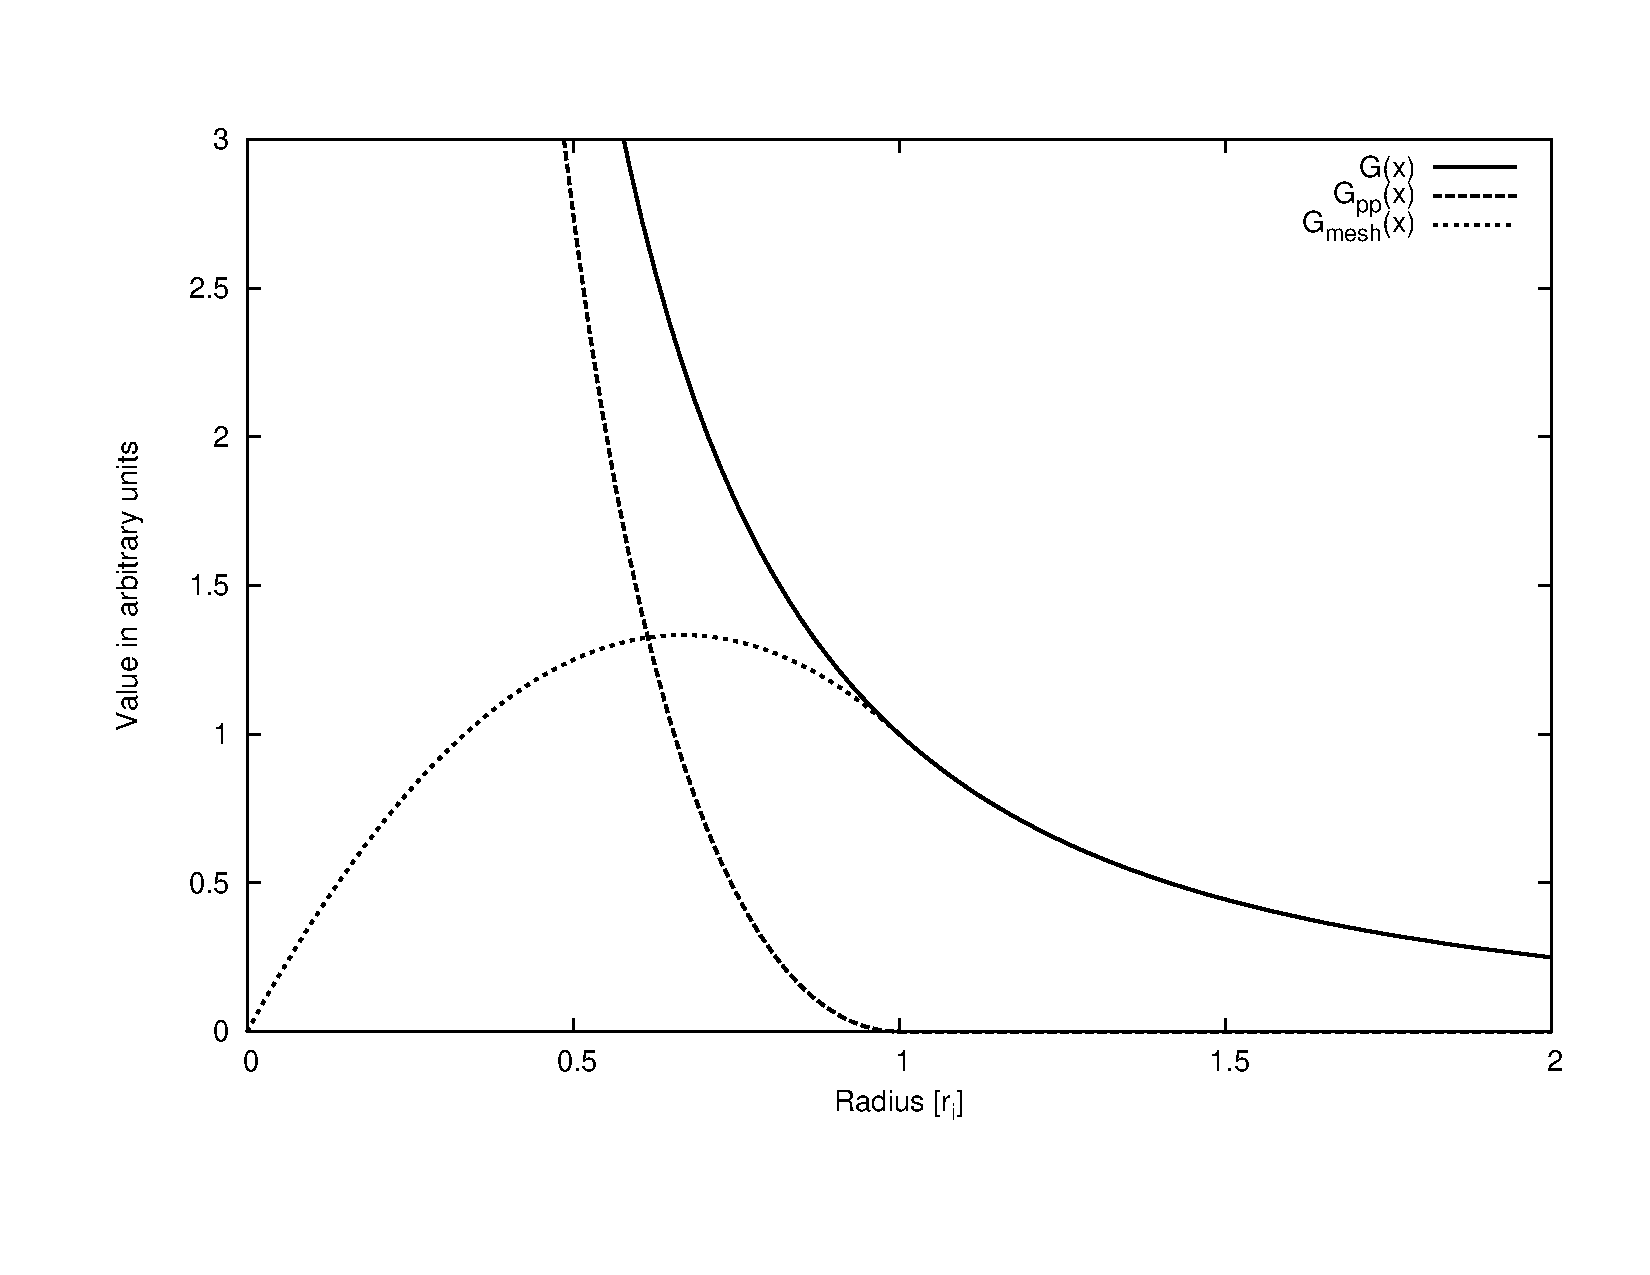
\includegraphics[width=\textwidth]{greens}
\caption{Decomposition of the Green function.}
\label{greensfunction}
\end{figure}

\begin{figure}[h!]
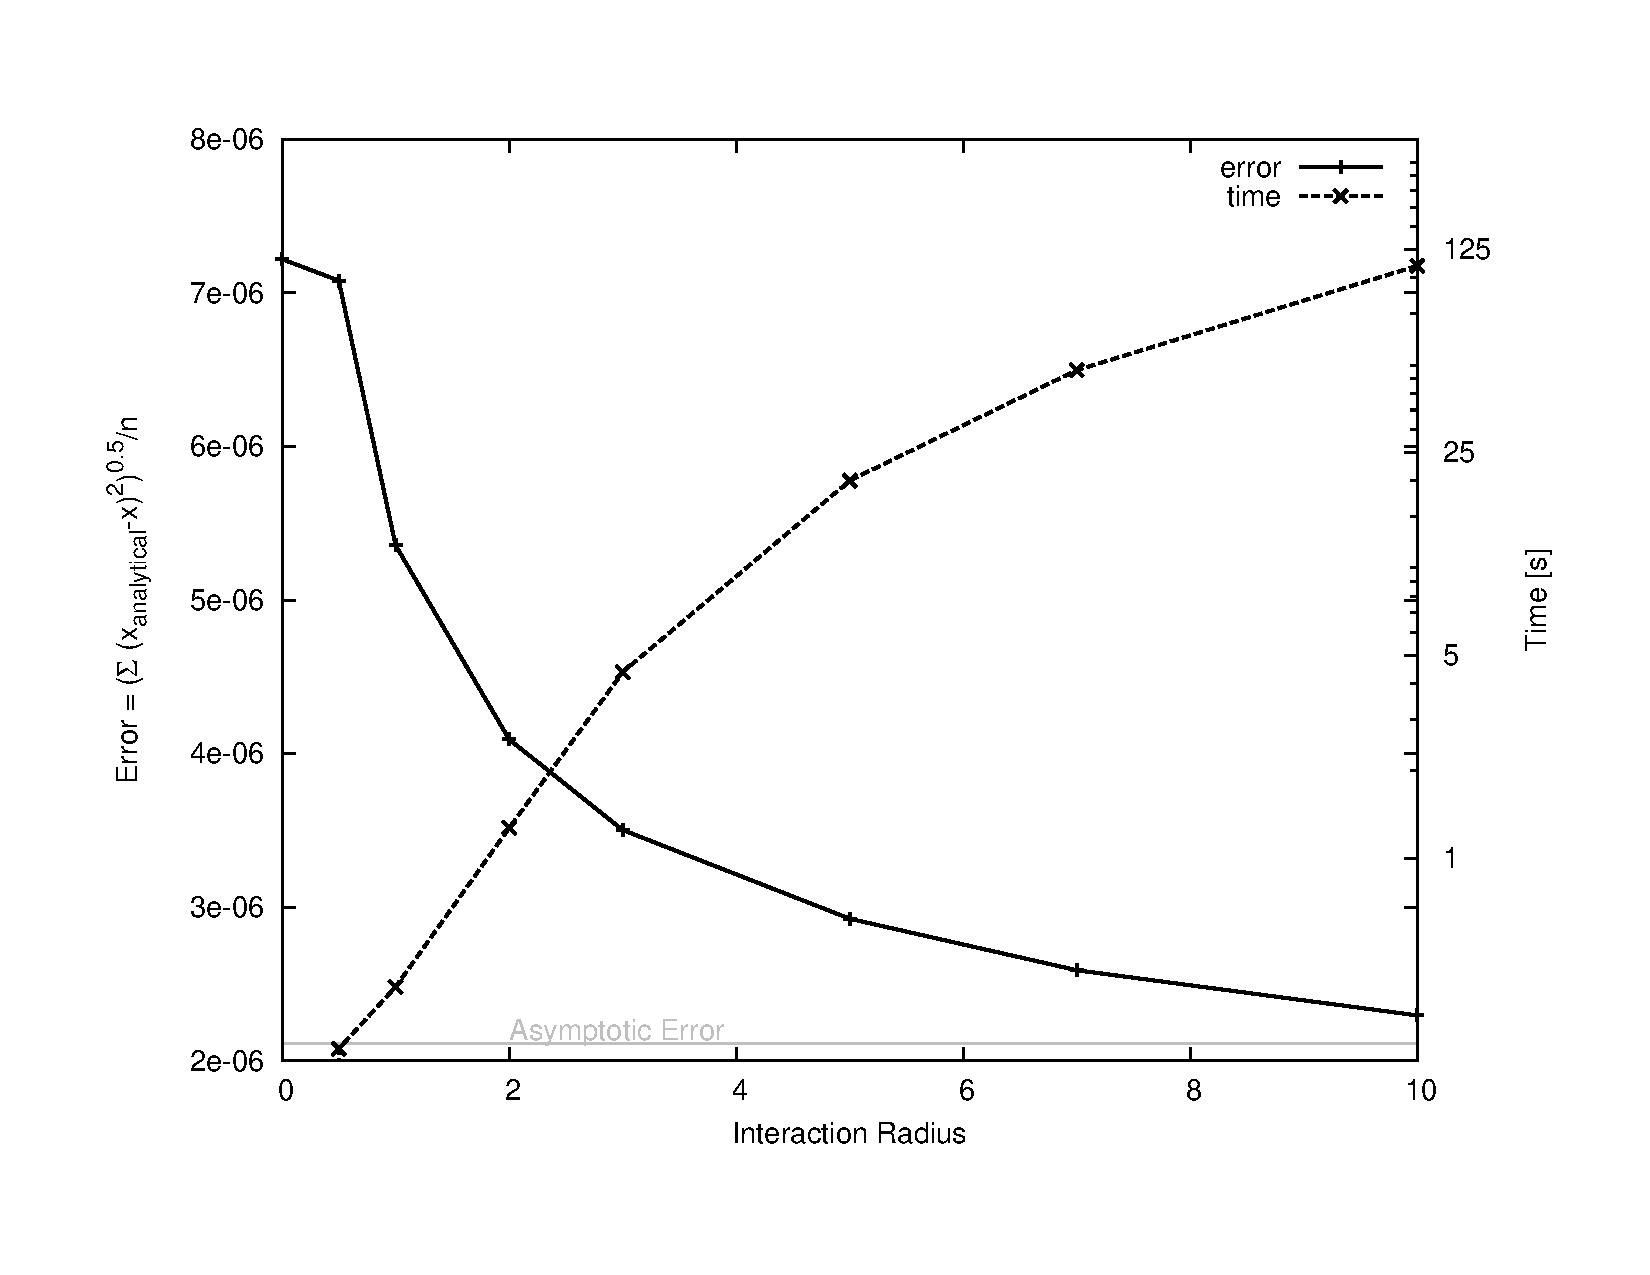
\includegraphics[width=\textwidth]{error_time}
\caption{Error and time scaling of the $P^3M$ solver for different interaction radii. Measured fo a uniform spherical
distribution of $10^4$ particles on 4 processors.}
\label{errortime}
\end{figure}
\pagebreak
Therefore the Green function from the PIC example has to be replaced by the following modified Green function:


\vspace{5mm}
\begin{code}
template<>
struct SpecializedGreensFunction<3> {
  template<class T, class FT, class FT2>
  //...

  template<class T, class FT, class FT2>
  static void calculate(Vektor<T, 3> &hrsq, FT &grn, FT2 *grnI, double R) {
    grn = grnI[0] * hrsq[0] + grnI[1] * hrsq[1] + grnI[2] * hrsq[2];
    grn = where(lt(R*R, grn), 1./sqrt(grn),
		((grn*sqrt(grn))/R-2*grn)/(R*R*R) + 2/R);
    grn[0][0][0] = grn[0][0][1];
  }   
};
\end{code}
\vspace{5mm}
The short range interaction is handled by IPPL's pairbuilding mechanism which applies
the Green function to each pair of particles whose distance is below the
interaction radius (see \ref{ppsection}). For this purpose \texttt{ChargedParticles} contains the following member
function:


\vspace{5mm}
\begin{code}
  void calculatePairForces(double interaction_radius)
  {
    HashPairBuilder< ChargedParticles<playout_t> > HPB(*this);
    //apply the field to each pair, the -1 is the field constant
    HPB.for_each(RadiusCondition<double, Dim>(interaction_radius), 
    			   ApplyField<double>(-1,interaction_radius));
  }
\end{code}
\vspace{5mm}
Which calls \texttt{ApplyField} for each pair of particles that fulfills the condition $||x_1-x_2|| = ||x|| <r_i$.
\clearpage
\pagebreak
\vspace{5mm}
\begin{code}
template<class T>
struct ApplyField {
  ApplyField(T c, double r) : C(c), R(r) {}
  void operator()(std::size_t i, std::size_t j, ChargedParticles<playout_t> &P) const
  {
    const Vector_t diff = P.R[i] - P.R[j];
    double sqr = 0;
    for(int d = 0;d<Dim;++d)
      sqr += diff[d]*diff[d];
		
     if(sqr!=0)
      {
	double r = std::sqrt(sqr);
	
	Vector_t Fij = C*(diff/r)*(1/sqr - (-3/(R*R*R*R)*r*r + 4/(R*R*R)*r));

	P.EF[i] -= P.Q[j]*Fij;
	P.EF[j] += P.Q[i]*Fij;
      }
  }
  T C;
  double R;
};
\end{code}

\section{Installation}
 \ippl uses the {\em cmake } build philosophy.  The following environment variables must be set
\begin{verbatim}
IPPL_ROOT
\end{verbatim} 
defining where \ippl is installed.

\subsection{Building \ippl}
\begin{verbatim}
cd $IPPL_ROOT
CXX=mpicxx F77=gfortran cmake -DCMAKE_VERBOSE_MAKEFILE=OFF
-DCMAKE_INSTALL_PREFIX=~/extlib/ippl $IPPL_ROOT
\end{verbatim}


\subsection{Building \ippl with Dynamic Kernel Scheduler}
To build \ippl with Dynamic Kernel Scheduler the DKS library must be built first. See the DKS readme file
for detailed instructions on DKS installation. The following environment variables must be set
\begin{verbatim}
$DKS_PREFIX
\end{verbatim}
defining where DKS library is installed.\\
To use DKS in \ippl it must be eneabled in CMakeLists.txt file. There are six options than can be set to
enable DKS for \ippl. Options ENABLE\_OPENCL, ENABLE\_CUDA and ENABLE\_OPENMP set which framework the 
DKS  was compiled with, at least one of these options needs to be set for \ippl to be able 
to use DKS. USE\_OPENCL, USE\_CUDA and USE\_MIC specifies which framework \ippl should use for DKS, only one 
option can be enabled at a time.\\ 
If Intel compiler is used to compile \ippl than DKS should also be compiled 
with intel compiler and OpenCL and OpenMP framworks can be enabled and used. If GNU compiler is used to compile 
\ippl DKS should also be compiled with GNU compiler and OpenCL and CUDA frameworks can be enabled and used. 
If \ippl is compiled with MPI compiler then DKS should also be compiled with MPI compiler to enable full MPI 
support in DKS.


\subsection{Used Compilers and Libraries}
The supported operating systems and libraries are listed in Table \ref{tab:archlib}.
\begin{table}[h]
  \caption{Supported Architectures and needed Libraries}
  \label{tab:archlib}
  \begin{center}
    \begin{tabular}{|lcccc|}
      \hline
      Operating System & HDF5  & H5hut & Compiler & Open MPI\\
      \hline
      Linux (SL) 2.6.18 & hdf5-1.8.5 & V0.99 & GNU 4.4.x, icc11.1 & 1.4.2 \\
      Cray XTx  & hdf5-1.8.5 & V0.99 & GNU 4.4 & - \\
      \hline
    \end{tabular}
  \end{center}
\end{table}





\clearpage
\section{Acknowledgements}
The contributions of various individuals and groups are acknowledged in the relevant chapters, 
however a few individuals have or had considerable influence on the 
development, Julian Cummings, Yves Ineichen and Jakob Progsch.
Misprints and obscurity are almost inevitable in a document of this size.
Comments and {\em active contributions}  from readers are therefore most welcome.
They may also be sent to \htmladdnormallink{\texttt{andreas.adelmann@psi.ch}}{mailto:andreas.adelmann@psi.ch}.

\subsection{Citation}
Please cite \ippl in the following way:
\begin{small}
\begin{verbatim} 
@techreport{ippl-User-Guide,
title = "{The IPPL (Independent Parallel Particle Layer)
              Framework }",
author = "A. Adelmann",
institution = "Paul Scherrer Institut",
number = "PSI-PR-09-05",
year = 2009}
\end{verbatim}
\end{small}


%& OPAL \\
% & V 1.0



\chapter{Framework Setup}
\label{sec:setup}

\section{Initialising \ippl}
\ippl is initialized by passing \texttt{argc} and \texttt{argv} to \texttt{Ippl()} constructor or by creating an instance of \texttt{Ippl::Options}, configuring it, and then passing that options object to \texttt{Ippl::initialize()}. After the \texttt{Ippl()} constructor call MPI (or any other parallel subsystem) is proper initialized. \\
With \texttt{Ippl::getNodes()} or \texttt{Ippl::myNode()} you can for example gather information how many compute nodes/cores are available and on which of the nodes you are running. \\
\begin{code} 
#include "Ippl.h"
int main(int argc, char *argv[])
{
    Ippl ippl(argc,argv);
    .....
\end{code}

\section{ Utility Classes in \ippl}
\ippl provides, and uses internally, a number of useful utility classes which you may find helpful when developing new applications. 

\subsection{Inform Class}
The Inform class is used to print messages to the console or to a file. It has an interface which is very similar to the iostream classes in C++, and it is mostly used in those situation where you might print a message to cout or cerr. An Inform object is created with a prefix string, which is then appended to all lines of output from the Inform object. Inform essentially takes in data to be printed, formats it for printing just as an ostream object would, but also appends the prefix message to all lines of output. Most important Inform will also indicate which node printed the message when running in parallel.

\subsubsection{Constructing New Inform Objects}

The constructor for Inform has the form 
\begin{smallcode}
Inform(char *prefix = 0, int node = 0)
\end{smallcode}
where prefix is a string to prepend to all output lines, and node indicates on what node the Inform object should actually print out the information it is given. Notice that both of these arguments have default values; if no arguments are used when creating a new Inform object, no prefix will be used, if only one argument is given, then node default to 0, which means this Inform object will only print out messages on node 0.
\begin{smallcode}
Inform blankmsg; 
blankmsg << "Some text." << endl; 
\end{smallcode}
This Inform object will print the text it is given to standard out. The final "\texttt{endl}" is a special manipulator object, which signals the Inform objec t to print out the message it has been given. It will automatically append an endline to the message if it does not already have one at the end. It is important to use endl with an Inform object if it is not ever used, the Inform object will never print out its accumulated text.
\begin{smallcode}
Inform testmsg("mytest"); 
testmsg << "More text. argc = " << argc << endl; 
\end{smallcode}
Here, the prefix is given, if this is used when running in serial, the output will look like:
\begin{smallcode}
mytest> More text. argc = 1 
\end{smallcode}
or, if you use this when there is more than one processor in use, the prefix will also include the node number in curly brackets:
\begin{smallcode}
mytest{0}> More text. argc = 1 
\end{smallcode}
On all other nodes than node 0, when this Inform object is used, it will not print out the message.
\begin{smallcode}
Inform testmsg("testall", INFORM_ALL_NODES); 
\end{smallcode}
This example is similar to the previous example, except the second argument explicitly specifies which node to print on. This can be a number from 0 .... (num nodes - 1), or, as in this example, it can be \texttt{INFORM\_ALL\_NODES} which indicates the message should be printed on ALL the nodes instead of just one. You can also change the node on which an Inform object will print after it has been created by using the \texttt{setprintNode(int)} method of \texttt{Inform}. 

\subsubsection{Predefined Inform Objects}
Creating new Inform objects for printing messages is useful in contexts where you would like a unique prefix to indicate where the message originated, say in a specific class method. However, the \ippl framework provides a set of predefined Inform instances which may be used to quickly generate output message or to make sure all messages have a common prefix. These Inform objects are static members of the IPPL class, which is used to initialize the framework. The predefined instances are:
\begin{smallcode}
IPPL::Info = new Inform ("IPPL") ; 
IPPL::Warn = new Inform("Warning"); 
IPPL::Error = new Inform("Error", INFORM_ALL_NODES);
\end{smallcode}
These three instances are used to print generally informative messages, warning messages, and error messages. \texttt{Info} and \texttt{Warn} only print on node 0 by default; \texttt{Error} will print on all nodes. You may use these to printmessages in your own application:
\begin{smallcode}
*IPPL::Info << "An informative message." << endl; 
\end{smallcode}
Notice that here that \texttt{Info} was first dereferenced, since it actually is a pointer to an \texttt{Inform} object. A better (and recommended) way to use these predefined instances is to use a macro which is defined for each instance. The macros to use are \texttt{INFOMSG}, \texttt{WARNMSG}, and \texttt{ERRORMSG}; an example of their use is:
\begin{smallcode}
WARNMSG("rhis is a warning: value = " << warnvalue << endl); 
\end{smallcode}
The argument to the macro is then given to the associated \texttt{Inform} object for printing. 

\subsection{Timer Class}
Timer is used to perform simple timings within a program for use in, e.g., benchmarking. It tracks real (clock) time elapsed, user time, and system time. It acts essentially as a stopwatch: 
initially it is stopped, and YOU tell it to stop and start with method calls. The Timer constructor takes no arguments; you create a new Timer object, and use the following methods:
\begin{smallcode}
//Start the clock running. Time only accumulates in the Timer when it is running. 
void start()
void stop()         //Stop the clock. The clock may be started again later. 
void clear()        //Resets the accumulated time to zero
float clock_time()  //Reports the accumulated "wall clock" time in seconds. 
float user_time()   //Reports theaccurnulated user CPU time in seconds. 
float system_time() //Reports the accumulated system CPU time in seconds. 
float cpu_time()    //Reports user_time() + system_time() 
\end{smallcode}

\clearpage

Example how to use the timer class: \\
\begin{code}

IpplTimings::TimerRef selfFieldTimer_m;    \\ definition

selfFieldTimer_m = IpplTimings::getTimer("computeSelfField");  
 
selfFieldTimer_m.start(); 
    /* compute something */
selfFieldTimer_m.stop();

IpplTimings::print();

\end{code}
Note on Cray XT3/4 only wall clock is reported. 

\subsection{Memory Footprint Class}
This class allows the application to query the amount of 
available memory. This feature will be available in V1.0.1.



\begin{verbatim}


\end{verbatim}





\begin{verbatim}


\end{verbatim}

\chapter{FFT}
\label{sec:fft}

The FFT class provides an interface for performing parallel Fourier transforms of various types on \ippl \texttt{\texttt{Field}} objects. FFT is templated on the type of transform to perform (\texttt{CCTransform}, \texttt{RCTransform}, or \texttt{SineTransform}); the dimensionality \texttt{\texttt{Dim}} of the fields to be transformed, and the floating-point precision type (either \texttt{float} or \texttt{double}). It is capable of transforming along all dimensions of a \texttt{\texttt{Field}} or only specified dimensions, and it handles all of the data transposes required to make the Fourier transforms efficient automatically. The FFT constructor arguments vary slightly depending upon which type of transform you wish to perform. Generally speaking, you provide an {\tt NDIndex} object or objects which contain the domains of the input and/or output \texttt{Field}s for the Fourier transform, an optional array of bools of length \texttt{Dim} indicating which dimensions are to be transformed (default is all dimensions), and an optional bool indicating whether or not to compress the intermediate \texttt{Field}s needed to perform data transposes when they are not in use. The default value of this optional argument is false, but the user can set this argument to true if it is necessary to conserve memory. For a complex--to--complex Fourier transform, the input and output fields are of the same element type and are the same size, so only one domain argument is needed. So in the simple case of transforming all dimensions of a \texttt{Field} of type {\tt complex<double>}, we would construct the FFT object with the code
\begin{smallcode}
FFT<CCTransform,Dim,double> ccfft(domain); 
\end{smallcode}
where domain is an {\tt NDIndex<Dim>} describing the domain of complex \texttt{Field}s to be transformed with the FFT object.
A real--to--complex Fourier transform takes a field of real numbers and returns a field of complex numbers (or vice-versa for an inverse complex--to--real transform), so we require separate domain arguments describing each \texttt{Field} in the FFT constructor. From the theory of Fourier mode analysis, we know that a Fourier transform of $N$ real numbers will produce $N/2+ 1$ unique complex modes, with modes $0$ and $N/2$ being purely real. Some FFT routines take advantage of the fact that if you pack together the real parts of modes $0$ and $N/2$ as one complex number, you can store all the resulting mode information in the same space as required for the input (i.e., $N$ real numbers or $N/2$ complex numbers). Such a technique tends to cause confusion in multidimensional real--to--complex FFTs, since mode data must then be separated out afterwards. So we choose a format in which the $N/2+ 1$ complex modes are stored separately as complex numbers. Thus, when a real--to--complex transform is performed on a {\tt \texttt{Field}} of doubles, the resulting {\tt \texttt{Field}} of type {\tt complex<double>} will have an extent one greater than half the length of the input field along the first dimension to be transformed and the same length along all other dimensions. This conformance of domains is checked by the FFT constructor. We might construct an FFT object for real--to--complex transforms with the line
\begin{smallcode}
FFT<RCTransform,Dim,double> rcfft(rdomain,cdomain,tdim); 
\end{smallcode}
where {\tt rdomain} and {\tt cdomain} are the conforming domains for the {\tt real} and {\tt complex} fields and {\tt tdim} is an array of bools indicating whether or not to transform each dimension. Note that we assume the axes of the field are to be transformed along in the order indicated by the domain arguments for a forward FFT and in the reverse order for an inverse FFT. Each \texttt{Index} object inside the provided domain should refer to a particular axis of the input \texttt{Field}, and these axes are transformed along in order. A sine transform is a special type of Fourier transform in which only the sine (odd) modes are retained. This transform has a field of real numbers for both its input and output, and its effect is to keep only that portion of the data which exhibits odd parity (i.e., vanishes at the endpoints of the interval). Typically, one wishes to enforce odd parity along one or more dimensions of a field, and then perform a standard real-to-complex transform along remaining dimensions. Hence, we require that the user provide two arrays of bools in the constructor: the first to indicate along which dimensions to perform a sine transform, and the second to indicate all of the transform dimensions (both sine transforms and standard FFTs). For example,
\begin{smallcode}
FFT<SineTransform,Dim,double> sinefft(rdomain,cdomain,sinedim,tdim);
\end{smallcode}
 

constructs an FFT object for doing sine transforms along the dimensions indicated by sinedim and a standard real-to-complex FFT over the other dimensions included in tdim. Alternatively, such transforms could be achieved in two steps, doing the sine transforms and the standard FFTs separately. In this case, we might construct our sine transform FFT object with the code
\begin{smallcode}
FFT<SineTransform,Dim,double> sinefft2(rdomain,sinedim); 
\end{smallcode}


and then construct a second FFT object for handling the real-to-complex transform. Note that a sine transform FFT object which is doing only sine transforms requires only a single domain argument describing the real input and output \texttt{Field}s in its constructor.

Once the appropriate FFT object has been constructed, a Fourier transform of data is invoked using the transform member function. The normal arguments to this function are an integer value of + 1 or -1 to indicate the sign of the exponential used in the transform (i.e., the direction of the transform, forward or inverse), and the input and output \texttt{Field}s. For this "two-field" form of the transform function, there is also an optional argument of type bool, which indicates whether or not the input \texttt{Field} is considered to be constant by the transform function. The default value of this optional argument is false, which allows the transform routine to attempt to use the input \texttt{Field} as temporary storage and avoid doing an additional data transpose. You should set the value of this argument to true if you must preserve the contents of the input \texttt{Field} for later use. We would use our previously constructed FFT object for real--to--complex transforms to perform a forward FFT in the following manner:
\begin{smallcode}
rcfft.transform(+l,realField,complexField);
\end{smallcode}
 

The results of the transform are automatically normalized such that a forward transform followed by an inverse transform returns the original data. For convenience, the FFT class has a member function \texttt{setDirectionName} which allows you to associate a character string with each of the transform directions + 1 and -1. You might choose to refer to these directions as "xtok" and "ktox", for example.

In the case of a complex-to-complex FFT or a pure sine transform; the input and output fields are the same size and of the same type. In these instances, we offer the option of performing the transform "in place"; that is, using just one \texttt{Field} argument for both the input and output. For example, we could perform an inverse complex-to-complex FFT with the code
\begin{smallcode}
ccfft.transform(-1,complexField2); 
\end{smallcode}



\subsection{Improving FFT Performance}
Some improvement in performance of the transform method may be obtained by careful selection of the axis ordering of input and output \texttt{Field}s. In order to perform a parallel FFT along a particular dimension, the FFT object will first reorder the axes so that the first axis is the one to be transformed. It does this by assigning the field data into a new \texttt{Field} with a domain in which the order of the original \texttt{Index} objects has been permuted. This new \texttt{Field},
which is maintained internally by the FFT class, has a data layout that is serial along this first dimension and parallel along all other dimensions. With this layout, each processor can independently perform FFTs along the serial axis for each of the one-dimensional strips of data it owns. To subsequently transform along another dimension, the FFT object must again transpose the data so that the next dimension to be transformed is now the first dimension and is serial. These data
transposes can be fairly costly to perform. We can eliminate at least one data transpose if the output \texttt{Field} supplied by the user has the same layout characteristics needed for the final transform (or, in the case of an "in place" transform, if the input \texttt{Field} matches the layout needed for either the first or last transform), and has no guard cell layers. For instance, let us assume we have a three-dimensional \texttt{Field} of complex numbers and we want to transform
all dimensions. If the \texttt{Index} objects {\tt I,J}, and {\tt K} describe the first, second, and third axes of our \texttt{Field} domain, we could perform a forward FFT with the line
\begin{smallcode}
ccfft.transform(+l,complexFieldl);
\end{smallcode}

If the first dimension of \texttt{complexField} is serial, the transform method will skip the first data transpose because the input data is already distributed appropriately for transforming along the first dimension. Similarly, if we were to call an inverse transform with this same \texttt{Field}, it would transform the axes in reverse order, and we would be able to skip the final data transpose. Alternatively, we might choose to do this FFT using separate input and output \texttt{Field}s:
\begin{smallcode}
ccfft.transform(+1,complexField1,complexField2); 
\end{smallcode}
In this case, the final optional argument to the "two-field" trans form function defaults to false, meaning that \texttt{complexFieldl} is not considered constant and may be used in place of a temporary \texttt{Field} to avoid the first data transpose. In addition, the output \texttt{Field} can be used in place of the final temporary \texttt{Field} if it has the proper layout. If \texttt{complexField2} has its axes reordered so that its first axis is the final axis to be transformed
(e.g., \texttt{K}, then \texttt{I}, then \texttt{J}) and that first axis is serial, then we can skip the final data transpose. This choice of data layout results in a slightly faster parallel FFT, and it is often convenient if all you need to do is transform the data, do a brief computation with the transformed data, and then invert the transform.

Another issue of relevance to the performance of the transform method is the type of routine used to perform the actual one-dimensional FFT. Currently, we provide two options for this. The first is Fortran 77 implementations of FFT routines from the Netlib repository. These are portable and highly optimized routines that we invoke via C++ wrapper functions. The second option (available only on SGI and Cray systems) is native FFT routines from the SGI/Cray Scientific Library. These routines can be substituted for the portable Netlib routines by supplying the option {\tt USE\_SCSL\_FFT} to the configure utility before compiling the \ippl library. These native library routines tend to be somewhat faster than the portable Fortran routines, and we plan to offer the ability to use native FFT routines such as FFTW in the future. 

\chapter{Particles}
\label{sec:particles}
This section describes the \ippl framework classes which provide the capability to performing particle-based simulations. We first describe how to design and instantiate \texttt{Particle} classes customized to the needs of a specific application, and then discuss the possible operations and expressions in which a particle object may be employed and end with an ready to use example.

\section{Basic \texttt{Particle} Object Characteristics}

The \ippl framework treats \texttt{Particle} classes as containers which store the characteristic data for \texttt{N} individual particles. Each particle has several attributes, such as position, mass, velocity, etc. Looked at in another way, \texttt{Particle} classes store several attribute containers, where each attribute container holds the value of that attribute for all \texttt{N} particles. \texttt{Particle} objects in \ippl may be thought of as shown in the following diagram: ...

There are two particle attributes predefined, namely R (position) and ID a global unique identifier.

The data type of each attribute, the number of attributes, and the names for these attributes are completely customizable, and are specified in the manner described in the following sections. Any number of different \texttt{Particle} classes may be defined and used within a given simulation. Also, the \texttt{Particle} objects may interact with \ippl \texttt{Field} objects or may be used independently. In addition to the attributes, each \texttt{Particle} object uses a specific layout mechanism, which describes the data of the individual particles is spread across the processors in a parallel environment. The \ippl framework provides several different \texttt{Particle} layout classes, any of which may be selected to partition the particle data among processors. The choice of layout depends on the intended use of the \texttt{Particle} object, as discussed later. Once defined and instantiated, \texttt{Particle} objects in the \ippl framework may be used in many ways, including:
\begin{itemize}
    \item Operations involving all the particles within a \texttt{Particle} object may be specified using simple expressions, in a manner very similar to that used for \texttt{Field} objects. These expressions may involve any of the attributes of the particles as well as other scalar data, and they may use not only the standard mathematical operators +, -, *, /, etc., but also standard mathematical functions such a s cos ( ) , exp ( ) , mod ( ) , etc.
    \item Alternatively, you may set up explicit loops that perform operations involving the attributes of a single particle or a subset of all the particles.
    \item \texttt{Particle}s may be created or destroyed during a simulation.
    \item \texttt{Particle}-to-\texttt{Field} and \texttt{Field}-to-\texttt{Particle} operations may be performed (e.g., a particular \texttt{Particle} attribute may be deposited onto a specified \texttt{Field} using a chosen interpolation method). 
\end{itemize}

\section{Defining a User-Specified \texttt{Particle} Class}

There is no specific class within the \ippl framework called \texttt{Particle}. Rather, the first step in deploying particles within a \ippl application is to define a user-specified \texttt{Particle} class, which contains the attributes required for each particle, as well as any, specific methods or data the user may need. To do this, the \texttt{ParticleBase} and \texttt{ParticleAttrib} classes are used, along with a selected subclass of the \texttt{ParticleLayout} class. The steps to follow in creating a new \texttt{Particle} class are:
\begin{itemize}
    \item Based on the type of interactions which the particles have with each other and with external objects such as a \texttt{Field}, select a method of distributing the particles among the nodes in a parallel machine.
    \item Next, decide what attributes each particle should possess.
    \item Third, create a subclass of \texttt{ParticleBase} which includes these attributes (specified as instances of the \texttt{ParticleAttrib} class template).
    \item Finally, instantiate this user-defined subclass of \texttt{ParticleBase} and create and initialize storage for the particles which are to be maintained by this object. 
\end{itemize}

The following sections describe in more detail how to accomplish these steps.

\subsection{Selecting a Layout: \texttt{ParticleLayout} and Derived Classes}

When used in a parallel environment, the \ippl framework partitions the particles in a \texttt{Particle} container among the separate processors and includes tools to spread the work of computing and the results of expressions involving \texttt{Particle} attributes among the processing nodes. There are, however, different ways in which particles may be distributed among the processors, and the method which should be used depends upon how the particles in a \texttt{Particle}
object will interact with each other and with \texttt{Field} objects (if at all). The \ippl framework includes different \texttt{Particle} layout mechanisms, which are all derived from the \texttt{ParticleLayout} class. Each \texttt{Particle} object needs its own layout object; that is, you cannot create a layout object and give it to more than one \texttt{Particle} object. The methods typically used to determine how to assign particles to particular nodes are based on analysis of the
position (\texttt{R} attribute) of each particle. Thus, \texttt{ParticleLayout} and its derived classes have two template parameters: the type and the dimensionality of the particle position attribute (this particle position attribute is discussed in more detail later). The following sections describe the particle layout mechanisms currently available in the \ippl framework.

\subsection{The \texttt{ParticleUniformLayout} Class}

The \texttt{ParticleUniformLayout} class maintains an equal number of particles on each node, with no consideration of particle position. \texttt{ParticleUniformLayout} is useful in those cases where particles do not interact with each other but perhaps with some other external agent, so that no consideration need be made about which particles are located near to others. In that case, with this layout maintains an equal balance of memory usage among the processors and requires relatively small amounts of interprocessor communication. If you require the ability to compute an interaction between a particle and its nearest neighbors, this is not the proper layout to use, in that case, the \texttt{Particle}SpatialLayout class (discussed next) is a better choice. The constructor for \texttt{ParticleUniformLayout} takes no arguments, but does require the two template parameters that specify the type and dimensionality of the particle position attribute. An example of creating a new \texttt{ParticleUniformLayout} instance for a 3D particle simulation is:
\begin{smallcode}
ParticleUniformLayout<double,3> uniformlayout();
\end{smallcode}


\subsection{The \texttt{ParticleSpatialLayout} Class}

\texttt{ParticleSpatialLayout}, in contrast to \texttt{ParticleUniformLayout}, assigns particles to nodes based upon their spatial location relative to a \texttt{FieldLayout}. It is useful when the particles will be interacting with other particles in their neighborhood or with a \texttt{Field} object. \texttt{ParticleSpatialLayout} will keep a particle on the same node as that which contains the section of the \texttt{Field} in which the particle is located. If the particle moves to a new position, this layout will reassign it to a new node when necessary. This will maintain locality between the particles and any \texttt{Field} distributed using this \texttt{FieldLayout}. Further more it will help keep particles which are spatially close to each other local to the same processor as well. As with all the layout classes, \texttt{ParticleSpatialLayout} requires the type and dimensionality of the particle position attribute as template parameters. The constructor for \texttt{ParticleSpatialLayout} takes one argument: a pointer to a \texttt{FieldLayout} object that tells the \texttt{ParticleSpatialLayout} how the \texttt{Field} is allocated among the parallel processors, so that the particles may be maintained local to this \texttt{Field}. Note that you do not, need to create a \texttt{Field} instance itself, you only need to give \texttt{ParticleSpatialLayout} a \texttt{FieldLayout} object. An example of creating an instance of this class is as follows:
\begin{smallcode}
FieldLayout<3> myfieldlayout(Index(l6), Index(16), Index(32)); 
ParticleSpatialLayout<double,3> myparticlelayout(&myfieldlayout);
\end{smallcode}


Note that the dimensionality of the \texttt{FieldLayout} and the \texttt{ParticleSpatialLayout} (in this example, 3) must be the same. You may also create a \texttt{ParticleSpatialLayout} instance without providing a \texttt{FieldLayout}. In this case, particles will remain on the node on which they were created. If at some future time you wish to provide a \texttt{FieldLayout} object to tell the \texttt{ParticleSpatialLayout} where to place the particles, you may do so using the \texttt{setFieldLayout} (\texttt{FieldLayout<Dim>*}) method of \texttt{ParticleSpatialLayout}. This is useful when reading particles in from an external source and the size of the spatial domain containing the particles is not known until all the particles have been read. The following example demonstrates the use of the capability:
\begin{smallcode}
ParticleSpatiaILayout<double,3> myparticleLayout; 
// calculate the size of the domain required to contain all the particles 
// create a new FieldLayout object based on these calculations 
FieldLayout<3> myfieldlayout(Index(minx, maxx), Index (miny, maxy), 
                             Index(minz,maxz);   
myparticlelayout.setFieldLayout(&myfieldlayout);
\end{smallcode}

\texttt{ParticleSpatialLayout} also provides functionality to maintain cached ghost particles from neighboring nodes which might be required for particle - particle interaction. A caching policy can be defined using the fourth template parameter of \texttt{ParticleSpatialLayout}:
\begin{smallcode}
typedef UniformCartesian<Dim, double> Mesh_t;
typedef ParticleSpatialLayout<double,Dim,Mesh_t,
        BoxParticleCachingPolicy<double, Dim, Mesh_t> > playout_t;
\end{smallcode}
The available chaching policies are: \texttt{NoParticleCachingPolicy},\texttt{BoxParticleCachingPolicy} and \texttt{CellParticleCachingPolicy}. With \texttt{NoParticleCachingPolicy} there is no caching whatsoever. \texttt{BoxParticleCachingPolicy} extends the interface of \texttt{ParticleSpatialLayout} by two functions \texttt{void setCacheDimension(int d, T length)} and \texttt{void setAllCacheDimensions(T length)} which are used to set the size of the cached region around the local domain in units of space. \texttt{CellParticleCachingPolicy} extends the interface of \texttt{ParticleSpatialLayout} by two functions \texttt{void setCacheCellRange(int d, int length)} and \texttt{void setCacheCellRanges(int d, int length)} which are used to set the size of the cached region around the local domain in units of grid cells of the mesh. \texttt{BoxParticleCachingPolicy} is the default policy.

The caching can be enabled or disabled by calling the \texttt{enableCaching()} or \texttt{disableCaching()} member functions of \texttt{ParticleSpatialLayout}. Caching is disabled by default.


\subsection{Selecting Particle Attributes: The \texttt{ParticleAttrib} \\Class}

\texttt{ParticleAttrib} is a class template that represents a single attribute of the particles in a \texttt{Particle} object. Each \texttt{ParticleAttrib} contains the data for that attribute for all the particles. Within a user-defined \texttt{Particle} class, you declare an instance of \texttt{ParticleAttrib} for each attribute the particles will possess and assigns to it an arbitrary name. \texttt{ParticleAttrib} requires one template parameter, the type of the data for the attribute. As an example, the statement:
\begin{smallcode}
ParticleAttrib<double> density; 
\end{smallcode}

declares an instance of \texttt{ParticleAttrib} named 'density', which will store a quantity of type double for all the particles of the \texttt{Particle} class that contains this data member.

\subsection{Specifying a User-Defined \texttt{Particle} Class: \\The \texttt{ParticleBase} Class}

\texttt{ParticleBase} is the class that all user-defined \texttt{Particle} classes must specify as their base class. It stores the list of attributes for the particles (which are maintained as instances of \texttt{ParticleAttrib}) and a selected parallel layout mechanism. In addition to providing all the capabilities for performing operations on the particles and their attributes, \texttt{ParticleBase} also defines two specific attributes which all user-defined \texttt{Particle} classes inherit:
\begin{smallcode}
ParticleAttrib<Vektor<T,Dim>>  R; 
ParticleAttrib<unsigned>      ID;
\end{smallcode}


The first attribute, \texttt{R}, represents the position of each particle. Each position is stored as a \texttt{Vektor<T, Dim>}, which is a \ippl data type representing a dim-dimensional vector with elements of type \texttt{T}. The second attribute, \texttt{ID}, stores a unique unsigned integer value for each particle. The values are not guaranteed to be in any particular order, but they are guaranteed to be unique for each particle. \texttt{ParticleBase} has one template parameter, the layout class to be used to assign particles
to processors (e.g., \texttt{ParticleSpatialLayout}). The data type and dimensionality of the particle position attribute (\texttt{R}) will be the same as those used to create the specific \texttt{ParticleLayout} derived class. Each \texttt{ParticleBase} contains one instance of the chosen layout class. There are two constructors for \texttt{ParticleBase}: a default constructor that creates a new instance of the layout class using the layout's default constructor, and a constructor which takes a pointer to an instance of the
layout class. The second version of the \texttt{ParticleBase} constructor is useful when the desired layout class requires arguments to its constructor (e.g., \texttt{ParticleSpatialLayout}, which may be give in a \texttt{FieldLayout} pointer).

Using \texttt{ParticleBase}, \texttt{ParticleAttrib}, and a selected class derived from \texttt{ParticleLayout,} you can create a user-defined \texttt{Particle} class using the following code template: \\
\clearpage
\begin{codeln}
class Bunch : public ParticleBase< ParticleSpatiaILayout<double,3> > 
{ 
public: 
    // Attributes for this particle class (besides position and ID). 
    ParticleAttrib<double>             qm;      // q/m ratio 
    ParticleAttribs Vektor<double,2> > vel; 	// velocity 

    // constructor 
    Bunch(Layout\_t *L) : ParticleBase<Layout\_t>(L) { 
        addAttribute(qm); 
        addAttribute(vel); 
    } 
}; 
\end{codeln}

Let us describe this example in detail by discussing the important lines in the order of use.

Line 1: You may select whatever name is appropriate for the specialized \texttt{Particle} class, but it must be derived from \texttt{ParticleBase}. 

In this case, we explicitly specify the type of layout to use (\texttt{ParticleSpatialLayout}), with particle position attribute type and dimensionality template parameters of double and 3, respectively. Alternatively, \texttt{Bunch} may have been declared as a class template itself and may have passed on the layout template parameters to \texttt{ParticleBase}. In that case, the first line would instead look like
\begin{smallcode}
template <class PLayout> 
class Bunch : public ParticleBase<PLayout> 
\end{smallcode}

Lines 5-6: Here is where the attributes for the particles in the \texttt{Particle} object are declared. They may be given any name other than \texttt{R} or \texttt{ID}. Instead of stating the type and dimensionality of this attribute specifically, you may also use one of the following typedefs and constants defined in \texttt{ParticleBase}:
\begin{itemize}
          \item \texttt{Dim} - the dimensionality of the particle position attribute (in this example, 3)
          \item \texttt{Position\_t} - the type of data used to store the position attribute components (here, this type is double)
          \item \texttt{Layout\_t} - a synonym for the specified layout class
          \item \texttt{ParticlePos\_t} - a typedef for the particle position attribute; it is shorthand for \texttt{ParticleAttrib< Vektor<Position\_t,Dim> >}
\end{itemize}
and could have been used to specify the attribute \texttt{vel} in the above example as \texttt{ParticlePos\_t vel};
\begin{itemize}
\item \texttt{ParticleIndex\_t} - a typedef for the particle global \texttt{ID} attribute; it is short for \texttt{ParticleAttrib<unsigned>} 
\end{itemize}
The constructor for this user-defined class must initialize \texttt{ParticleBase} with a pointer to an instance of the selected layout class. 

In this example, the layout class is \texttt{ParticleSpatialLayout}, but using one of the typedefs listed above, we can abbreviate this as \texttt{Layout\_t}. Note that we only define one constructor here, omitting the default constructor. This is done because \texttt{ParticleSpatialLayout} (which we have hard-coded as the layout for this user-defined \texttt{Particle} class) requires an argument to its constructor, and this can only be provided if we use a constructor for our \texttt{Particle} class as shown here. A new instance of this class would be declared in an application as follows:
\begin{smallcode}
Bunch myBunch (new ParticleSpatialLayout<double,3>(myFieldLayout)); 
\end{smallcode}
where my\texttt{FieldLayout} was a \texttt{FieldLayout} object created previously. The only action that is required in the constructor for the derived class is to inform the base class of the declared attributes, 
using the \texttt{addAttribute(.)} method of \texttt{ParticleBase}, which registers the specified \texttt{ParticleAttrib} instance with the parent class \texttt{ParticleBase}. The order in which attributes are registered is not important.

\subsection{Example \texttt{Particle} Classes: The \texttt{Genparticle} and \texttt{GenArrayParticle} Classes}
The \ippl framework provides two classes which are examples of \texttt{Particle} classes derived from \texttt{ParticleBase}: \texttt{Genparticle} and \texttt{GenArrayParticle}. They may be used as samples from which to build new classes, or they may be used to quickly include particle capabilities in an application. \texttt{Genparticle} is a \texttt{Particle} class with three attributes: \texttt{R} and \texttt{ID} inherited from \texttt{ParticleBase}, and an attribute named data with elements
of an arbitrary type. \texttt{Genparticle} has two template parameters: the type of particle layout to use and the type \texttt{T} of attribute data. It has two constructors just as \texttt{ParticleBase} does: the default and one taking a layout pointer. An example of instantiating a \texttt{GenParticle}object is shown below.
\begin{smallcode}
GenParticle<ParticleUniforrnLayout<float,3>,UserDefinedType> GP(); 
\end{smallcode}


\texttt{GenArrayParticle} is almost identical to \texttt{GenParticle}, the difference being that \texttt{GenArrayparticle} contains not just one but an array of attributes data \texttt{[0 ... N-l]} of a specified type. The number of elements in the attribute array, \texttt{N}, is given as a third template parameter. The following example shows a \texttt{GenArrayParticle} being created with 5 floats stored in the data array for each particle:
\begin{smallcode}
GenArrayParticle<ParticleSpatialLayout<doulble,3>,float,5> GAP(
        new ParticleSpatialLayout<double,3>(myFieldLayout)); 
\end{smallcode}

It is important to note that the array data in \texttt{GenArrayParticle} contains a set of particle attributes of the same type. In situations where it is necessary to have a variety of particle attribute types, you may use the \texttt{Genparticle} class with the type of data being specified as a user-defined struct containing the various attributes needed.

\subsection{Using \texttt{Particle} Classes in an Application}

After a specific \texttt{Particle} class has been defined and created in a \ippl application, you may create and initialize new particles, delete unwanted particles, and perform computations involving these particles. This section describes how to accomplish these tasks.

\subsection{Creating New \texttt{Particle}s}

When a \texttt{Particle} object is created, it is initially empty. Storage for new particles is allocated using the create (unsigned) method of \texttt{ParticleBase}. For example, if a \texttt{Particle} object bunch has been created already, the statement
\begin{smallcode}
bunch.create(100); 
\end{smallcode}


will allocate storage for 100 new particles. All the attributes for the particles in the \texttt{Particle} object will have this new storage allocated. The data is uninitialized, except for the global \texttt{ID} attribute; you must assign the proper values to the position and any other attributes that have been defined. The new storage is appended to the end of any existing storage.

\texttt{ParticleBase} includes two methods that allow you to query how many particles exist. The function \texttt{getTotalNum()} will return the total number of particles being stored among all the processors; the function \texttt{getLocalNum()} will return the number of particles just on the local node. Although the new storage space is allocated on the local processor on which the call to create was executed, the \texttt{Particle} class will not officially add the particles to its
local count (and will not tell any other processors it has created these new particles) until you call the \texttt{update()} method of \texttt{ParticleBase}. Thus, a call to \texttt{getLocalNum()} will report the same number just before and just after the call to create. The storage does exist after create is called, but only after the \texttt{update} method (which is discussed in more detail in a later section) has been called will all the processors have correct information on their local and total particle counts.

\subsection{Initializing Attribute Data}

After calling create to allocate new storage, you must initialize the data. This should be done after calling create and before calling \texttt{update} for the \texttt{Particle} object. After the data is initialized, the \texttt{update} routine will properly distribute the particles to their correct node based on the layout mechanism chosen for that \texttt{Particle} object and possibly the positions of the particles as set during their initialization. The following example shows one way to initialize the data for newly
created particles when running on a single-processor machine. (This example will be modified in the following section for the case of running in parallel.) \\
\begin{code}
// create and'initialize data for an instance of Bunch 
Bunch myBunch(new Bunch::Layout\_t(myFieldLayout)); 
int currLocalPtcls = myPtcls.getLocalNum(); 
myBunch.create(100); 
for (int i = 0; i < 100; i++) { 
    myBunch.R[currLocalPtcls + i] = Vektor<double,3>(0.0, 1.0, 0.0); 
    myBunch.vel[currLocalPtcls + i] Vektor<double,3>(1.0, 1.0, 1.0); 
} 
myBunch.update(); 
\end{code}


In this example, 100 new particles are created, and the \texttt{R} and \texttt{vel} attributes are initialized to \texttt{Vektor} quantities. Notice that each attribute is accessed simply by specifying it as a data member of the \texttt{myBunch} object. After create was called, even though the 100 particles were not added to the \texttt{Particle} object's count of local particles, the storage was allocated and it was possible to assign values to the new elements in the attribute storage
(accessed simply using the \texttt{[]} indexing operator). Finally, calling \texttt{update} added the new storage to the count, of particles stored in \texttt{myBunch}. Further calls to getLocalNum and getTotalNum would report the proper values.

\subsection{Initializing Attribute Data on Parallel Architectures}

The code shown in the previous example has one problem when used on parallel architectures: the call to create is performed on each processor, so if there were P processors a total of 100*P particles would be created. This may be the desired behavior, if so, the previous example is sufficient. However, if you are reading data on particle positions and other attributes from a file or some other source, you may wish to create particles on a single processor, and then distribute the
data to the proper nodes. To do this, you need to call create and assign initial data on only one node but call update on all the processors. The \texttt{singlelnitNode()} method of \texttt{ParticleBase} will return a boolean value indicating whether the local processor should be used to create and initialize new particles in this way. The following example demonstrates how to use this method for initializing particles: \\
\begin{code}
// create and'initialize data for an instance of Bunch 
Bunch myBunch(new Bunch::Layout\_t(myFieldLayout)); 
int currLocalPtcls = myPtcls.getLocalNum();
if (myBunch.singleInitNode()) { 
    myBunch.create(100);  
    for (int i = 0; i < 100; i++) { 
        myBunch.R[currLocalPtcls + i] = Vektor<double,3>(0.0, 1.0, 0.0); 
        myBunch.vel[currLocalPtcls + i] Vektor<double,3>(1.0, 1.0, 1.0); 
    }
} 
myBunch.update(); 
\end{code}


\subsection{Deleting \texttt{Particle}s}

\texttt{Particle}s may also be deleted during a simulation. The method \texttt{destroy (unsigned M, unsigned I)} of \texttt{ParticleBase} will delete \texttt{M} particles, starting with the \texttt{I}th particle. The index \texttt{I} here refers to the local particle index, not the global \texttt{ID} value. Thus \texttt{I = 0} means delete particles starting with the first one on the local processor.

Unlike the situation when creating new particles, the storage locations for the deleted particles will not be removed from attribute data storage until \texttt{update} is called. Instead, the requests to delete particles are cached until the update phase, at which time all the deletions are performed. You are allowed to issue multiple delete requests between \texttt{update}s. For example, if there are 100 particles on a local node, and you request to delete particles 0 to 10
and then request to delete particles 60 to 70, nothing will change in the attribute storage until you call \texttt{update}, and no change will occur to the local and total particle counts until \texttt{update()} is complete.

\subsection{Updating \texttt{Particle}s: The \texttt{update()} Method}

The \texttt{update()} method of \texttt{ParticleBase} is responsible for making sure that all processors have correct information about how many particles exist and where they are located in a parallel machine. As mentioned previously, \texttt{update} must be called by all processors after a sequence of particle creation or deletion operations. The \texttt{update} method is also responsible for maintaining a proper assignment of particles to processors, based on the particular
\texttt{ParticleLayout} class used to create the
\texttt{ParticleBase} object. Typically, this layout mechanism depends on the position of particles, so when particles change their position, they may need to be reassigned to a new processor to maintain the proper layout. In this case, the \texttt{update} method should be called whenever a computation is complete which alters the attributes (e.g. position) that a layout depends upon. The following short example demonstrates using \texttt{update} in conjunction with some operation that alters the x-coordinate of a
set of particles. \\
\begin{code}
// do some computation involving myBunch for several time steps 
while (computation_done == false) { 
    // for each particle, add some constant to the x coordinate 
    myBunch.R(0) += 0.li 
    // update the Particle object; this may move particles between nodes 
    myBunch.update(); 
    // determine if the computation is done, etc.
}
\end{code}

\subsection{Using Particle Attributes in Expressions}

Computations involving particle attributes may be performed in many ways. Data-parallel expressions that involve all particles of a given \texttt{Particle} object may be used, or specific loops may be written that employ attribute iterators or nearest-neighbor pairlist iterators.

\subsubsection{Attribute Expressions}

Just as with the \texttt{Field} class, you may perform data-parallel operations on particle attributes using a simple expression syntax, which the \ippl framework will translate into efficient inlined code. These operations will be performed for every particle. The expressions may include any of the attributes in a \texttt{Particle} object as well as scalar values, may use mathematical operators such as +, -, *, / etc., and may call standard mathematical functions such as \texttt{cos(
)}, \texttt{exp( )}, \texttt{mod( )} , etc. for an attribute value of each particle. Some examples are shown below.
\begin{smallcode}
double dt = 2.0; 
myBunch.R += myBunch.vel* dt; 
myBunch. vel = 1. � - log (1. � + myBunch. R * myBunch. R) ; 
myBunch.update(); 
\end{smallcode}


Attribute expressions will perform their operations on all the particles in the \texttt{Particle} object, including any new particles allocated via a call to create, even before update has been called. This fact is useful when initializing the attributes for newly created particles (e.g., to set the init value for some scalar quantity to zero). Generally, however, unless you are performing an initialization of new particles, you should avoid using particle expressions of this type after calls to create or destroy and before a call to update.

Some attributes, such as \texttt{Vektor}s or \texttt{Tenzor}s, have multiple components, and you may wish to involve only the \texttt{N}th component of the attribute in an expression. To do so, use the \texttt{()} operator to select the \texttt{N}th component of that attribute. For instance, using \texttt{myBunch} from the previous example, you can change just the x-coordinate of the particle position attribute \texttt{R} as follows: 
\begin{smallcode}
myBunch.R(0) = myBunch.R(l) - cos(myBunch.R(2));
\end{smallcode}


For 2D or 3D quantities, use two or three indices. For example, if rho is a 3x3 \texttt{Tenzor} attribute of myBunch, you can do the following:
\begin{smallcode}
myBunch.rho(0,0) = -(myBunch.rho(0,l) + myBunch.rho(0,2)); 
\end{smallcode}

Attribute expressions may also use the where operator in much the same way as for \texttt{Field} expressions. The first argument to where is some expression that results in a \texttt{boolean} value for each particle. The second and third arguments are expressions that will be evaluated for a particle if the first argument is \texttt{true} or \texttt{false}, respectively, for that particle. For example,
\begin{smallcode}
myBunch.vel = where(myBunch.R(0) > 0.0, -2.0 * myBunch.vel, myBunch.vel) 
\end{smallcode}

changes the value of the \texttt{vel} attribute in \texttt{myBunch} when the x-coordinate of the particle position is positive.

\subsection{\texttt{Particle} Iterator Loop}

You also have the capability of performing operations on specific particles using iterators or standard indexing operations. The \texttt{ParticleAttrib} containers in a \texttt{Particle} class may be used just as regular \texttt{STL} containers. The \texttt{begin()} and \texttt{end()} methods of the \texttt{ParticleAttrib} class will return an iterator pointing to the first element and just past the last element, respectively, of the attribute. These iterators may be used in an explicit loop just as if they were pointers into the attribute array.
\begin{smallcode}
ParticleAttrib<unsigned>::iterator idptr, idend = myBunch.ID.end(); 
for (idptr = myBunch.ID.begin(); idptr != idend; ++idptr) 
    cout << "Particle ID value: " << *idptr << endl; 
\end{smallcode}


Iterators are available for all \texttt{ParticleAttribs}. As an alternative, you may simply use the \texttt{[]} operator to access the attribute data of the \texttt{N}th particle on a node, treating \texttt{ParticleAttrib} as a regular array of data.
\begin{smallcode}
int nptcls = myBunch.getLocalNum(); 
for(int i=0; i < nptcls ++i) { 
    cout << "Particle ID value: " << myPtcls.ID[i] << endl; 
}
\end{smallcode}


\section{Nearest-Neighbor Interactions (Jakob)}

%A standard need for many types of particle simulation is the execution of some calculation involving an interaction between one particle and all other particles within a given interaction region or radius. The interaction may involve particles that are on other processors, so it is important to efficiently communicate the necessary data between the nodes and limit the amount of work used in determining the nearest-neighbor interaction pairlists. For this type of computation,
%\texttt{ParticleBase} provides a specialized iterator, called \texttt{pair\_iterator}, which allows you to iterate over all neighbors of a given particle. The specific layout mechanism used by a \texttt{Particle} object takes care of calculating which particles lie within a selected interaction radius of each other, taking into account nearby particles which may reside on other processors in a parallel machine. The first step in calculating nearest-neighbor interactions is to specify what constitutes the
%neighborhood. Currently, only a radially symmetric interaction neighborhood is supported in \ippl. The interaction radius may be the same for each particle, or it may be a scalar attribute of the \texttt{Particle} class (of the same type as that used for the particle coordinates, e.g., \texttt{double} or \texttt{float}). Before any nearest-neighbor calculation is performed, you must specify the interaction radius of the particles. This is done using the
%\texttt{setInteractionRadius()} method of \texttt{ParticleBase}, giving as an argument either a single scalar value that will be used for all the particles, or a \texttt{ParticleAttrib<T>} quantity. In the latter case, each particle can have a different interaction radius. \texttt{ParticleBase} will remember this data and use it in the calculation of interaction lists. You may call these methods more than once; the most recent value given for the interaction radius is used to determine the
%nearest-neighbor pairlists. After changing the interaction radius, you should as always perform an \texttt{update()} to make sure all nodes have correct information on how to find neighboring particles. You may, for example, update the \texttt{ParticleAttrib} used to store the individual particle interaction radii as the last step of some calculation, and then call \texttt{update()}. You can retrieve the interaction radius for any local particle by calling the method
%\texttt{getlnteractionRadius(unsigned)} of the \texttt{Particle} object containing that particle.

%The second step in this process is to retrieve a list of nearest-neighborparticles for a given local particle, and then to perform the desired calculation using those nearby particles. This is done using the 
%\begin{smallcode}
%getpairlist(unsigned, pair_iterator&, pair_iterator&)
%\end{smallcode}
%method of \texttt{ParticleBase}. The first argument is the local index of the central particle under consideration. The second and third arguments are, set equal to begin and end
%\texttt{pair\_iterator} objects for the specified particle. The type \texttt{pair\_iterator} is defined in \texttt{ParticleBase}. This set of \texttt{pair\_iterator} objects is then used to retrieve the local indices of all particles within the interaction region of the central particle.

%Here is an example of how to use this mechanism: \\
%\clearpage
%\begin{codeln}
%myBunch.setlnteractionRadius(4.0); //determines interaction region 
%Bunch::pair_iterator neighbor, neighbor_end;
%for(int i=0; i < myBunch.getLocalNum(); ++i;) { 
%    myBunch.getPairlist(i, neighbor, neighbor_end);
%    for ( ; neighbor != neighbor_end; ++neighbor) { 
%        User\texttt{Particle}::pair\_t pairdata = *neighbor; 
%        int n = pairdata.first; 	           // local index of next neighbor 
%        double sep2 = pairdata.second;         // distance^2 between particles 
%        myBunch.R[i] += myBunch.vel[n] * 2.0;  // any calculation c<;>uld be here 
%    }
%}
%myPtcls.update();
%\end{codeln}
%On line 2, we declare the iterators used to obtain the beginning and end of the list of particle neighbors. These iterators are set in the call to \texttt{getpairlist} on line 4. Of particular note is how the data for each neighbor is obtained from the iterator, as done in lines 6-8: dereferencing the iterator returns an object of type \texttt{ParticleBase:: pair\_t}, which stores a pair of values the local index of the neighboring particle, and the square of the distance
%between the particles. The index and separation are obtained by accessing the member data elements \texttt{first} and \texttt{second}, respectively, of the \texttt{pair\_t} object.


\subsection{\texttt{Particle} - \texttt{Particle} Interactions}
\label{ppsection}
Efficient particle - particle interactions can be achieved by use of \texttt{PairBuilder} objects. The basic usage is as follows:

\begin{smallcode}
PairBuilder< Bunch<ParticleLayout_t> > PB(myBunch);
PB.for_each(PairCondition(), PairFunctor());
\end{smallcode}
This will call PairFunctor for each pair of particles that fulfills the PairCondition. There are three PairBuilders available: \texttt{HashPairBuilder}, \texttt{BasicBairBuilder} and \texttt{SortingPairBuilder}. HashPairBuilder should be used in most cases since it has the best time complexity. There are three predefined \texttt{PairConditions}. \texttt{TrueCondition} is always true and can be used to iterate over all pairs, \texttt{RadiusCondition} is true for each pair that is closer than a given interaction radius and \texttt{BoxCondition} is true for each pair where one particle lies inside a bounding box around the other particle. The following code shows how to iterate over all pairs within a given interaction radius:

\begin{smallcode}
struct PairFunctor{
  void operator()(std::size_t i, std::size_t j, Bunch<ParticleLayout_t> &P) const
  {
    //some interaction involving particles i and j
  }
};


HashPairBuilder< Bunch<ParticleLayout_t> > HPB(myBunch);
HPB.for_each(RadiusCondition<double, Dim>(interaction_radius), PairFunctor());
\end{smallcode}

To correctly generate all pairs in a multi process simulation a caching strategy has to be chosen so each process also has the required ghost particles. To achieve this for the example given one would call 

\begin{smallcode}
PL->setAllCacheDimensions(interaction_radius);
PL->enableCaching();
\end{smallcode}
with \texttt{PL} being the \texttt{ParticleSpatialLayout} of the bunch.

It is also possible to write custom pair conditions. These have to provide a \texttt{operator()} that takes two vectors and returns a bool, when the functor is used, it is passed two vectors that represent the particle positions. Additionally pair conditions have to provide a \texttt{getRange} function that takes an integer as input and returns the ``radius'' along that dimensions for which the pair condition can be true. In other words: for two particle positions \texttt{a} and \texttt{b} for which the pair condition returns true, the condition \texttt{|a[i] - b[i]| <= getRange(i)} must hold.

\subsection{\texttt{Particle} - \texttt{Field} Interactions}

%\section{\texttt{Particle} - \texttt{Field} Interactions}

Many particle-based simulation methods, including "particle-in-cell" (PIC) simulations, rely on the ability of particles to interact with field quantities. For instance, in particle-based accelerator (plasma) simulations, you typically track the motions of charged plasma particles in a combination of externally applied and self-generated electromagnetic fields. In a \ippl application, such fields might be stored as \texttt{Field} objects of type \texttt{Vektor} existing on a pre-defined mesh. Particles moving through this mesh must be able to "gather" the current value of a \texttt{Field} to their exact positions. Additionally, in order to compute the values of self-generated fields, the particles must be able to "scatter" the value of an attribute onto nearby mesh points, producing a \texttt{Field}. These gather/scatter operations are done using a set of \ippl interpolation methods.

\ippl provides a hierarchy of interpolation classes, each derived from the base class \texttt{Interpolate} and each containing the basic \texttt{gather} and \texttt{scatter} functions. The \texttt{gather} method allows you to gather one or more specified \texttt{Field}s into an equal number of \texttt{ParticleAttribs}. Similarly, \texttt{scatter} will accumulate one or more \texttt{ParticleAttribs} on to an equal number of \texttt{Field} objects. An example of how to scatter the particle density to a \texttt{Field} is shown below.
\begin{smallcode}
InterpolateNGP<Dim> mylnterpolater(myBunch);           // create NGP interpolater 
Field<double,Dim> ptcl_density(myfieldlayout);         // create density field 
myInterpolator.scatter(myBunch.density,ptcl_density);  // do scattet 
\end{smallcode}
The various classes derived from \texttt{Interpolate} implement these \texttt{gather} and \texttt{scatter} methods using different well-known interpolation schemes, such as nearest grid point (NGP), linear interpolation, and the subtracted-dipole scheme (SUDS). You may use these provided classes as a template for deriving new classes from \texttt{Interpolate} that implement other interpolation schemes of interest.

In case of the CIC Interpolation and non-cyclic boundary condition, care has to be taken to not place particles in the outer half of boundary cells. Otherwise values will be scattered out of the grid and be irretrivable.

\chapter{Using the \texttt{Field} and Related Classes}

This section introduces the interface of the \texttt{Field} class and related classes. We describe how
to instantiate \texttt{Field} objects, use \texttt{Index} objects to perform index operations, perform expression
operations with overloaded operators, apply boundary conditions, use the where construct for
conditionals, invoke reduction operations, and use mathematical functions.

\section{\texttt{Field} Object Instantiation}

\subsection{\texttt{Field} Template Parameters} \label{sec:tmpl_params}

The \texttt{Field} class is parametrized on 4 template parameters: type \texttt{T}, dimensionality \texttt{Dim},
mesh type \texttt{Mesh}, and centering \texttt{Centering}.
\begin{smallcode}
Field<class T, unsigned Dim, class Mesh=UniformCartesian<Dim,MFLOAT=doub1e>,
      class Centering=Mesh::DefaultCentering>
\end{smallcode}
The \texttt{T} parameter represents the type of data that can be stored inside of a \texttt{Field}. Currently,
the \texttt{Field} class supports the intrinsic types \texttt{bool, int, float, double}. One may use any
user-defined type or class as the template parameter; however, one must also add traits to the
framework to implement the desired data-parallel promotion properties so that \texttt{Field} operations
work. The framework includes 
\begin{smallcode}
Vektor<Dim, T>, Tenzor<Dim , T>, SymTenzor<Dim, T> 
\end{smallcode}
classes\footnote{The strange spellings avoid conflicts with other classes such as the STL vector class.}
, which are (mathematical) vectors, tensors, and symmetric tensors whose
elements are of type \texttt{T}. Traits are implemented in these classes so that they may serve as elements
of fully-functional \texttt{Field} objects.
The \texttt{Dim} parameter represent the dimensionality of the \texttt{Field} that is being constructed. This
must correspond to the \texttt{Dim} parameters in all other objects used to construct the \texttt{Field}.
The \texttt{Mesh} parameter represents the mesh on which the field is discretized. \ippl
pre-defines two appropriate classes (\texttt{Cartesian} and \texttt{UniformCartesian}) to use for this
parameter, one of which serves as the default value of the \texttt{Field} ``Mesh'' template parameter:
\texttt{UniformCartesian<Dim, double>}. Refer to the \ippl User Refercnce for details on the
\texttt{UniformCartesian} class; basically, it represents a \texttt{Cartesian} mesh with uniform grid spacings. 
The \texttt{Cartesian} class represents a cartesian mesh with nonuniform grid spacings. NB.:
the type parameter \texttt{MFLOAT} for \texttt{Cartesian} represents only the data type used to store internal
information like mesh spacing values; if \texttt{double} satisfies the user, he need not specify it.

The \texttt{Centering} parameter represents the centering of the field on its mesh. \ippl
pre-defines \texttt{Cell} and \texttt{Vert} classes to represent cell and vertex centering, and has implementations 
of appropriate mechanisms for \texttt{Cartesian} and other classes which use them. \ippl
also predefines a \texttt{CartesianCentering} class to represent more general centerings--combinations 
of vertex and cell centering direction-by-direction and component-by-component for
\texttt{Field}s with multicomponent element types such as \texttt{Vektor}. Finally, \ippl predefines a
wrapper class \texttt{CommonCartesianCenterings} with typedef’s several common special
cases to represent face and edge centerings, for example, refer to the \ippl User Reference
for details.

\subsection{Invoking the \texttt{Field} Constructor} \label{sec:inv_field}

There are six steps in the general construction of a \texttt{Field}:
\begin{enumerate}
    \item Construct \texttt{Index} objects, one for each dimension of the \texttt{Field}. The \texttt{Index} objects describe the desired index domain along the axis.
    \item Construct an \texttt{NDIndex} object with the dimensions of the \texttt{Field}. A single \texttt{NDIndex} object contains N \texttt{Index} objects, and fully describes the total index domain.
    \item Populate the \texttt{NDIndex} with the \texttt{Index} objects created in step 1.
    \item Construct a \texttt{FieldLayout} object with the \texttt{NDIndex} object. The \texttt{FieldLayout} object will control how the data of a specified \texttt{Field} object will be partitioned among physical nodes in a parallel environment.
    \item If desired, construct \texttt{BConds} and \texttt{GuardCellSizes} objects for specifying boundary conditions and guard-cell layers, respectively. If unspecified, these default to no-op and zero.
    \item Finally, construct a \texttt{Field} with the \texttt{FieldLayout}, \texttt{BConds}, and \texttt{GuardCellSizes} object as arguments to the constructor. This target \texttt{Field} must be parametrized as described in Section \ref{sec:tmpl_params}. The \texttt{Dim} template parameter must match the one for the \texttt{FieldLayout} and other objects involved, or you will get a compiler error.
\end{enumerate}

For the cases of a 1,2, or 3 dimensional \texttt{Field}, you may omit steps 2 and 3; instead directly pass the one, two, or three \texttt{Index} objects as arguments to the \texttt{FieldLayout()} constructor. The \texttt{Dim} template parameter must match the number of \texttt{Index} objects passed or you will get a compiler error.

The following code segment demonstrates the construction of a single two dimensional \texttt{Field} of \texttt{double}'s using the six-step method described above: \\
\begin{code}
unsigned Dim = 2;
int Nx = 100, Ny = 50;
Index I(Nx), J(Ny)l                 // Step 1
NDIndex<Dim> domain;                // Step 2
domain[0] = I;                      // Step 3
domain[1] = J;                      // Step 3
FieldLayout<Dim> layout(domain);    // Step 4
Field<double, Dim> A(layout);       // Step 5
\end{code}

The following three examples show the construction of a 3 dimensional \texttt{Field} without the intermediate \texttt{NDIndex} construction:
\begin{smallcode}
Index I(100), J(5), K(25);
FieldLayout<3> layout(I,J,K);
Field<double, 3> A(layout);
\end{smallcode}

You may also construct \texttt{Field} via copy constructor, wherein a \texttt{Field} is copied into another \texttt{Field}. This results in an element-by-element copy of the data: 
\begin{smallcode}
// assuming we have constructed a 2D Field of doubles in A
A = 2.0;
Field<double, Dim> B(A);
// B now contains the values 2.0 everywhere
\end{smallcode}

\section{The \texttt{Index} Class}

The \texttt{Index} class represents a strided range of indices, and it is used to define the index extent of \texttt{Field} objects on construction and to reference subranges within \texttt{Field}'s in expressions. The constructor for \texttt{Index} takes one, two or three int arguments. In the case of three arguments, these represent the base index value, the bounding index value and the stride. The two and one-argument cases are simplifications, with the one-argument case being qualitatively different; in
particular,
\begin{smallcode}
Index I(8);
\end{smallcode}
instantiates an \texttt{Index} object representing the range of integers from $0$ to $7$ inclusive, with implied stride $1$. The two-argument
\begin{smallcode}
Index J(2,8);
\end{smallcode}
instantiates an \texttt{Index} object representing the range of integers $[2,8]$, with implied stride 1. The three-argument
\begin{smallcode}
Index K(1,8,2);
\end{smallcode}
instantiates an \texttt{Index} object representing the range of integers $[1,8]$, with stride 2; that is the ordered set $\{1,3,5,7\}$.

Note that the single argument in the one-argument case defines the number of elements, rather than the bound. This means that \texttt{Index J(8)}, which represents $[0,7]$, is different than \texttt{Index J(0,8)} and \texttt{Index J(0,8,1)}, which both mean $[0,8]$.

As illustrated in Section \ref{sec:inv_field}, you use \texttt{Index}'s in constructing the \texttt{FieldLayout} object which goes into the \texttt{Field} constructor. The sizes of the \texttt{Index}'s used to construct the \texttt{FieldLayout} determine the size of the \texttt{Field} in each dimension; here size means the number of integers in the range represented by the \texttt{Index}. For example, the following code segment instantiates a 3-dimensional \texttt{Field A} having size 5 in the first dimension, size 9 in the second dimension, and size 4 in the
third dimension: \\
\begin{code}
unsigned Dim = 3;
int Nx = 5;
int Ny = 9;
int Nx = 4;
Index I(Nx), J(Ny), K(Nz);
FieldLayout<Dim> layout(I,J,K);
Field<double, Dim> A(layout);
\end{code}

You can also use \texttt{Index} objects for initializing \texttt{Field} elements with integer ranges of values. This and more typical use of \texttt{Index} object in conjunction with \texttt{Field} objects is discussed in Section \ref{sec:index_fields}.

Finally, \ippl defines various operators on \texttt{Index} objects, mostly used to represent finite-different stencil operations on \texttt{Field}'s, as described in Section \ref{sec:index_fields}. If
\begin{smallcode}
Index I(8);
\end{smallcode}
is an \texttt{Index} object representing $[0,7]$, then the expression
\begin{smallcode}
I - 1
\end{smallcode}
represents the range of the same length offset by $-1$, or $[-1,6]$. Similarly, the expression
\begin{smallcode}
I + 1
\end{smallcode}
represents $[2,8]$.

\section{The \texttt{NDIndex} Class}

The \texttt{NDIndex} class is primarily a container which holds \texttt{N} \texttt{Index} objects. It is templated on the spatial dimension \texttt{N}, and the constructor takes \texttt{N} \texttt{Index} arguments. For example: 
\begin{smallcode}
Index I(5), J(9), K(4);
NDIndex<3> Domain(I, J, K);
\end{smallcode}

An \texttt{NDIndex} object appears as an array of \texttt{Index} objects; you may access the \texttt{Index} object for and dimension using the \texttt{[]} operator. For example:
\begin{smallcode}
Index tmpJ = Domain[1];
\end{smallcode}

\section{The \texttt{FieldLayout} Class}

\texttt{FieldLayout} is the class responsible for determining where the data in a \texttt{Field} object is located. It is templated on the number of indices for the \texttt{Field}; when constructing a new \texttt{FieldLayout} object, you must tell it what is the index range for each dimension (or axis). A single \texttt{NDIndex} object may be used as the argument to a new \texttt{FieldLayout} instance:
\begin{smallcode}
Index I(5), J(9), K(4);
NDIndex<3> Domain(I, J, K);
FieldLayout<3> Layout(Domain);
\end{smallcode}
Or, possibly more conveniently, you may just specify the N \texttt{Index} objects to the constructor of the \texttt{FieldLayout} directly, without explicitly creating an \texttt{NDIndex} object:
\begin{smallcode}
Index I(5), J(9), K(4);
FieldLayout<3> Layout(I, J, K);
\end{smallcode}

\subsection{Specifying Serial or Parallel Layout}

By default, a \texttt{FieldLayout} object will partition all \texttt{N} dimensions in a parallel fashion. For example a 2D \texttt{Field} with indices running from $0 \ldots 5$ in each dimension, created with a \texttt{FieldLayout} specified as follows:
\begin{smallcode}
Index I(6), J(6);
FieldLayout<3> Layout(I, J);
\end{smallcode}
will have both the \texttt{I} and \texttt{J} indices partitioned across the nodes in parallel. This would lead to a layout something like that shown in the following figure, if there are four nodes:

TODO: BILD

Unless you tell it otherwise, \texttt{FieldLayout} will attempt to distribute the data among the processors by subdividing each dimension in turn until it has the proper number of subregions. Those axes which are considered for subdivision are the \textit{parallel} axes, which means that a given node will only contain \texttt{Field} data for a subset of the indices along that dimension. You can, however, tell \texttt{FieldLayout} which axes to subdivide, and which to maintain as \textit{serial}. Serial axes are
not ever partitioned by \texttt{FieldLayout}. You must have at least on parallel dimension in a given \texttt{FieldLayout}; by default, all axes are parallel.

To specify serial axes, you provide additional arguments to the \texttt{FieldLayout} constructor, using the keywords \texttt{SERIAL} or \texttt{PARALLEL}. If you create a new \texttt{FieldLayout} by just specifying \texttt{N} \texttt{Index} objects, then you may provide up to \texttt{N} more arguments to the constructor to set the corresponding dimension's layout method. For example, we may change the earlier example of a 2D \texttt{Field} to have the second dimension use a serial layout as follows:
\begin{smallcode}
Index I(6), J(6);
FieldLayout<3> Layout(I, J, PARALLEL, SERIAL);
\end{smallcode}
In this case, the data would be partitioned into four subregions like the following (the horizontal direction is the first dimension, the vertical direction the second)

TODO: BILD

If an \texttt{NDIndex} object is used to create the \texttt{FieldLayout} instead of several \texttt{Index} objects, to change the default layout style you must instead provide an array of keywords (of type \texttt{e\_dim\_tag}) specifying the layout for the \texttt{N} dimensions. For example: \\
\begin{code}
Index I(5), J(9), K(4);
NDIndex<3> Domain(I, J, K);
e_dim_tag ParallelMethod[2];
ParallelMethod[0] = PARALLEL;
ParallelMethod[1] = SERIAL;
ParallelMethod[2] = SERIAL;
FieldLayout<3> Layout(Domain, ParallelMethod);
\end{code}

\section{Boundary Condition Classes}

One of the great frustrations in using data parallel objects is the proper representation of boundary conditions. Most data parallel environments (such as HPF or CMFortran) require that one perform special operations to observe periodic or reflected behaviour at the boundary. This requirement obscures the original clarity of the index notation. You construct \texttt{Field} objects within the \ippl framework using \texttt{BConds} boundary condition object which defines the behaviour of \texttt{Field} and \texttt{Field}
indexing operations at the boundaries. This makes the same, clear indexing notation do the right thing under a variety of imposed boundary conditions.

\subsection{Available Boundary Conditions}

\ippl pre-defines classes to represent 6 different forms of boundary conditions:
\begin{enumerate}
    \item Periodic boundary condition: \texttt{PeriodicFace}
    \item Positive reflecting boundary condition: \texttt{PosReflectFace}
    \item Negative reflecting boundary condition: \texttt{NegReflectFace}
    \item Constant boundary condition: \texttt{ConstantFace}
    \item Zero boundary condition (special case of constant): \texttt{ZeroFace}
    \item Linear extrapolation boundary condition: \texttt{ExtrapolateFace}
\end{enumerate}

They represent boundary conditions for a single dimension of a (possibly) multidimensional field, for one ``side'' (or face) of the mesh along that dimension. That is, you must specify two boundary condition objects for each dimension of the \texttt{Field} -- one for each face of the mesh along that dimension. These classes are parametrized on the same four template parameters as \texttt{Field} (see Section \ref{sec:tmpl_params}); the defaults for \texttt{Mesh} and \texttt{Centering} are
\texttt{UniformCartesian} and \texttt{Cell}. As a
further refinement, you may specify boundary conditions for individual components of multicomponent \texttt{Field} elements such as \texttt{Vektor}.

\subsection{Using Boundary Conditions With \texttt{Field}s}

The \texttt{BConds} class is a container for the individual specialized boundary conditions; this is the argument passed to the \texttt{Field} constructor. A \texttt{BConds} object acts very much like an array of boundary conditions: when first created, the \texttt{BConds} object is empty, and you add new boundary condition objects to it by treating it as a vector and assigning to its elements. The basic procedure is to construct a \texttt{BConds} object, then construct new or use existing boundary condition objects (from the list
above) to fill it, as illustrated in this example: \\
\begin{code}
unsigened Dim = 2;
Index I(4), J(4);
BConds<double, Dim> bc;
bc[0] = new PeriodicFace<double, Dim>(0);
bc[1] = new PeriodicFace<double, Dim>(1);
bc[2] = new PeriodicFace<double, Dim>(2);
bc[3] = new PeriodicFace<double, Dim>(3);
Field Layout<Dim> layout(I, J);
Field <double, Dim> A(layout, GuardCellSizes<Dim>(1), bc);
\end{code}
Again, the individual face boundary condition objects (in this example, \texttt{PeriodicFace}) perform their task for only a single face of the mesh. In this way, there may be different types of boundary conditions in different dimensions. The face boundary-condition constructors take an unsigned argument designating the face according the following numbering convention: The integers 0 and 1 apply to the boundaries of the first coordinate direction where 0 represents the negative face and 1
represents the positive face. The integers 2 and 3 apply to the boundaries of the second coordinate direction where 2 represents the negative face and 3 represents the positive face. This pairing of integers and domains continues into higher dimensions. The constructors also take optional second and third unsigned parameters to specify a single \texttt{Field} element component rather than all of them. Refer to the \ippl User Reference for more details on these classes, and a detailed discussion
of how the various boundary conditions affect \texttt{Field} operations.

\subsection{Default Boundary Condition}

If a \texttt{Field} is constructed with no \texttt{BConds} object specified, the default is for that \texttt{Field} to have NO boundary conditions. In that case, the boundary conditions container within the \texttt{Field} is empty. It is possible to add additional boundary conditions for a specific face to a \texttt{Field} after it has been constructed; to do so, retrieve the boundary condition container from the \texttt{Field} using the method \texttt{Field::getBConds()}, and then add new face-specific boundary conditions to the returned
\texttt{BConds} container object as shown in the previous example.

\section{The \texttt{GuardCellSizes} Class}

A \texttt{GuardCellSizes} class, an optional argument to the \texttt{Field} constructor, represents the maximum separation (in elements) of \texttt{Field} elements which will be combined in \texttt{Field} expressions. Typically, this reflects the order of finite differencing in stencil operations. The primary reason for guard cells is parallelism -- a \texttt{Field} domain-decomposed into multiple subdomains with data from adjacent subdomains, so that the stencil operations
have all required data locally. The \texttt{GuardCellSizes}
class is parameterized on the unsigned value \texttt{Dim}, which represents the number of dimensions of the \texttt{Field} object. This \texttt{Dim} value must match the corresponding parameter value of the \texttt{Field} object.

The constructor for \texttt{GuardCellSizes} takes either one or two arguments, which are either \texttt{unsigned} or \texttt{unsigned*}. The one-argument forms specify the same number of guard layers for all dimensions; the two-argument forms specify different numbers for the right and left faces; the unsigned forms specify the same number of layers for all dimensions; and the \texttt{unsigned*} forms specify different number of layers for the different dimensions: 
\begin{smallcode}
GuardCellSizes(unsigned s);  // Same no. left&right, same for all directions
GuardCellSizes(unsigned *s); // Same no. left&right, value for each direction
// Diff. left&right, same for all directions
GuardCellSizes(unsigned l, unsigned r); 
// Diff. left&right, value for each direction
GuardCellSizes(unsigned *l, unsigned *r); 
\end{smallcode}

Section \ref{sec:index_fields}, ``Using \texttt{Index} Objects with \texttt{Field}'s'', shows examples using \texttt{Field} indexing to implement stencil operations. It discusses the numbers of guard layers required by one of the examples.

\section{Operations on \texttt{Field} Objects}

\subsection{Assignment}

A single line of code which contains an assignment operator and a \texttt{Field} on the left hand side of the assignment operator is called a \texttt{Field} expression. Many different terms may appear on the right-hand side of a \texttt{Field} expression (or as the second argument in an \texttt{assign()} call as described below). These include scalars, \texttt{Index}'s, \texttt{Field}'s and \texttt{IndexingField}s's. Currently because of the lack of template member functions in
C++ compilers, you must use the \texttt{assign()} function rather than the
\texttt{operator=}:
\begin{smallcode}
assign(Lhs, Rhs);
\end{smallcode}
where \texttt{Lhs} and \texttt{Rhs} are \texttt{Field} expressions. When template member functions become available, you will simply write:
\begin{smallcode}
Lhs = Rhs
\end{smallcode}

Refer to the \ippl Users Reference for more details, and examples showing where you may use \texttt{operator=} and where you must use \texttt{assign()}. The following are examples of legal assignments:\\
\begin{code}
unsigned Dim = 2, int N = 100;
Index I(N), J(N);
FieldLayout<Dim> layout(I, J);
Field<double, Dim> A(layout), B(layout), C(layout);
A = 2.0;
assign(A, 2.0 + B);
assign(B, A + 2.0);
assign(B[I][J], 3.0 + B[I][J]);
assign(A[I][J], I + A[I][J]/C[I][J]);
\end{code}

For cases where more than one term exists on the right hand side of an assignment, the \texttt{assign()} call must be made. Any combination of scalars, \texttt{Field}'s, \texttt{IndexingField}'s (indexed \texttt{Field} objects; see Section \ref{sec:index_fields}), and \texttt{Index}'s can be put as the second argument of the \texttt{assing()} call. The only requirement in combining terms is that the appearance of an \texttt{Index} object anywhere inside of an expression requires that all the \texttt{Field} objects contained in the expression must be indexed. It
is not possible to combine \texttt{Field}'s and \texttt{IndexingField}'s in a single expression. Nor is it possible to combine \texttt{Field}'s and \texttt{Index} objects in a single expression.

Another intermediate solution to accommodate the lack of member function templates (and therefore the ability to use the \texttt{operator=} member function with more than one term on the right hand side of an expression) is the utilization of the accumulation operators (since this does not require member function templates). Thus, instead of writing
\begin{smallcode}
assign(A, 4.0 + B);
\end{smallcode}
one could write
\begin{smallcode}
A = 0.0;
A += 4.0 + B;
\end{smallcode}
This technique can be used with any of the accumulation operators (\texttt{+=,-=,*=,/=}).

\subsection{Using \texttt{Index} Objects with \texttt{Field}'s} \label{sec:index_fields}

The \texttt{Field} object works intimately with \texttt{Index} objects to perform a wide variety of operations. Use the \texttt{Index} object to specify the access pattern into a data parallel \texttt{Field} object. Do this by using \texttt{Index} objects inside the brackets following a \texttt{Field} object as follows:
\begin{smallcode}
A[I][J] = B[I][J];
\end{smallcode}
A \texttt{Field} object followed by brackets containing \texttt{Index} objects is called an \texttt{IndexingField}, because \ippl internally uses an \texttt{IndexingField} class as the return value for the \texttt{Field::operator[]}.

You can use \texttt{Index} objects to initialize a \texttt{Field} with integer range data -- that is, assign to a strided range of \texttt{Field} elements the values of a strided range of integers multiplied by the element type. This only works of multiplication by an int is defined for the \texttt{Field} element type, which it is for the intrinsic types $\{$\texttt{int, float, double, bool}$\}$ and the \ippl pre-defined \texttt{Field} element classes $\{$\texttt{Vektor, Tenzor,
SymTenzor}$\}$. For multidimensional \texttt{Field}'s, the range of values is replicated along
the other dimensions. For example, given a \texttt{Field} that is size 8 in its first dimension and size 4 in its second dimension, the code segment
\begin{smallcode}
assign(A[I][J], I);
\end{smallcode}
produces the following values in the \texttt{Field A}:
%
   \begin{center}
        \begin{tabular}{|c|c|c|c|c|c|c|c|}
        \hline
        0 & 1 & 2 & 3 & 4 & 5 & 6 & 7 \\
        \hline
        0 & 1 & 2 & 3 & 4 & 5 & 6 & 7 \\        \hline
        0 & 1 & 2 & 3 & 4 & 5 & 6 & 7 \\        \hline
        0 & 1 & 2 & 3 & 4 & 5 & 6 & 7 \\        \hline
        \end{tabular}
   \label{tbl:t1}
   \end{center}
%
(Here, as in subsequent figures like this displaying \texttt{Field} values, the positive direction of the first coordinate is from left to right and the positive direction for the second coordinate is from top to bottom.) Likewise, an assignment of the form
\begin{smallcode}
assign(A[I],[J], J);
\end{smallcode}
produces
%
   \begin{center}
        \begin{tabular}{|c|c|c|c|c|c|c|c|}
        \hline
        0 & 0 & 0 & 0 & 0 & 0 & 0 & 0 \\        \hline
        1 & 1 & 1 & 1 & 1 & 1 & 1 & 1 \\        \hline
        2 & 2 & 2 & 2 & 2 & 2 & 2 & 2 \\        \hline
        3 & 3 & 3 & 3 & 3 & 3 & 3 & 3 \\        \hline
        \end{tabular}
   \label{tbl:t2}
   \end{center}

The \texttt{Index} objects used to access ranges of values in a \texttt{Field} object do not have to be the same \texttt{Index}'s used in constructing the \texttt{FieldLayout} object used to construct the \texttt{Field}. You can use \texttt{Index} objects of smaller size to access a subrange of the \texttt{Field}. For example, if we wanted to have an 8 by 8 \texttt{Field} with zeros everywhere except for a 4 by 4 subregion in the center, the following code segment would accomplish this goal: \\
\begin{code}
unsigned Dim = 2;
Index I(8), J(8);
Index I2(2,5), J2(2,5);
FieldLayout<Dim> layout(I, J);
Field<double, Dim> A(layout);
A = 0.0;
A[I2][J2] = 1.0;
\end{code}
This would produce the following values in the \texttt{Field A}:
%
   \begin{center}
        \begin{tabular}{|c|c|c|c|c|c|c|c|}
        \hline
        0 & 0 & 0 & 0 & 0 & 0 & 0 & 0 \\        \hline
        0 & 0 & 0 & 0 & 0 & 0 & 0 & 0 \\        \hline
        0 & 0 & 1 & 1 & 1 & 1 & 0 & 0 \\        \hline
        0 & 0 & 1 & 1 & 1 & 1 & 0 & 0 \\        \hline
        0 & 0 & 1 & 1 & 1 & 1 & 0 & 0 \\        \hline
        0 & 0 & 1 & 1 & 1 & 1 & 0 & 0 \\        \hline
        0 & 0 & 0 & 0 & 0 & 0 & 0 & 0 \\        \hline
        0 & 0 & 0 & 0 & 0 & 0 & 0 & 0 \\        \hline
        \end{tabular}
   \label{tbl:t2}
   \end{center}

The lower-limiting case range for an \texttt{Index} object is, of course, a single element. For this case you can just use an integer constant or variable; the following assigns a single element of the \texttt{Field A}: \\
\begin{code}
Index I(4), J(4);
FieldLayout<2> layout(I, J);
Field<double,2> A(layout);
A = 0.0;
A[1][1] = 1.0;
\end{code}
The resultant \texttt{Field A} contains the values:
%
   \begin{center}
        \begin{tabular}{|c|c|c|c|}
        \hline
        0 & 0 & 0 & 0 \\        \hline
        0 & 1 & 0 & 0 \\        \hline
        0 & 0 & 0 & 0 \\        \hline
        0 & 0 & 0 & 0 \\        \hline
        \end{tabular}
   \label{tbl:t2}
   \end{center}

The typical use for indexing is stencil operations, using \texttt{Index} expressions adding or subtracting integer constants to represent the finite differences. This amounts to global data transformation upon a \texttt{Field} through the use of \texttt{Index} operations. For example, if a 4 by 4 \texttt{Field} named \texttt{A} is initialized as follows: \\
\begin{code}
unsigned Dim = 2;
int N = 4;
Index I(N), J(N);
FieldLayout<Dim> layout(I, J);
Field<double, Dim> A(layout, GuardCellSizes<Dim>(1));
assign(A[I][J], I + 1);
\end{code}
then the values in the \texttt{Field A} will be:
%
   \begin{center}
        \begin{tabular}{|c|c|c|c|}
        \hline
        1 & 2 & 3 & 4 \\        \hline
        1 & 2 & 3 & 4 \\        \hline
        1 & 2 & 3 & 4 \\        \hline
        1 & 2 & 3 & 4 \\        \hline
        \end{tabular}
   \label{tbl:t2}
   \end{center}

Now, let's form another \texttt{Field}, \texttt{B}, and assign to it the value of an \texttt{IndexingField} of A which represents an indexed operation:
\begin{smallcode}
Field<double, Dim> B(layout);
assign(B[I][J], A[I+1][J]);
\end{smallcode}

Here we see that the \texttt{Field A} has been indexed with something other than a plain \texttt{Index} object. Rather, it has been indexed by an index expression. The \texttt{Index} objects have been overloaded to allow addition and subtraction by integers to produce other \texttt{Index} objects. The framework recognizes this operation as requesting that all the data in \texttt{A} be shifted to the left (along the first dimension in the negative direction) by 1 position. The \texttt{Field B} contains the values:
%
   \begin{center}
        \begin{tabular}{|c|c|c|c|}
        \hline
        2 & 3 & 4 & 0 \\        \hline
        2 & 3 & 4 & 0 \\        \hline
        2 & 3 & 4 & 0 \\        \hline
        2 & 3 & 4 & 0 \\        \hline
        \end{tabular}
   \label{tbl:t2}
   \end{center}

\texttt{Index}ing operations which access data beyond a \texttt{Field} boundary set the target positions to zero. For the reminder of this section, we shall assume this zero valued boundary condition (which is the default condition when no boundary condition is specified). A variety of boundary conditions can be set on each boundary of a \texttt{Field} and are discussed in detail in the next section.

The \texttt{GuardCellSizes} object used to construct \texttt{Field A} in this example must specify at least on guard layer in the 1st dimension, to accommodate the ``$+1$'' in the indexing operation. The one used, \texttt{GuardCellSizes<Dim>(1)} allows ``$+/-1$'' indexing (as in a width-one stencil), and also allows width-one stencils in the 2nd dimension, because the use of the unsigned argument (the constant, 1) specifies one guard layer both left and right for all directions.

Had we wished to shift the \texttt{Field A} down (along the second dimension in the negative direction) we could have written
\begin{smallcode}
assign(B[I][J], A[I][J+1]);
\end{smallcode}
Then the values in the \texttt{Field B} are:
%
   \begin{center}
        \begin{tabular}{|c|c|c|c|}
        \hline
        1 & 2 & 3 & 4 \\        \hline
        1 & 2 & 3 & 4 \\        \hline
        1 & 2 & 3 & 4 \\        \hline
        0 & 0 & 0 & 0 \\        \hline
        \end{tabular}
   \label{tbl:t2}
   \end{center}

You can shift in the positive or negative direction on any \texttt{Index} object used to index a \texttt{Field}. For example, \\
\begin{code}
unsigned Dim = 2;
int N = 4;
Index I(N), J(N);
FieldLayout<Dim> layout(I, J);
Field<double, Dim> A(layout, GuardCellSizes<Dim>(1));
assign(A[I][J], I + J + 1);
\end{code}
will initialize the values in the \texttt{Field A} to:
%
   \begin{center}
        \begin{tabular}{|c|c|c|c|}
        \hline
        1 & 2 & 3 & 4 \\        \hline
        2 & 2 & 4 & 4 \\        \hline
        3 & 4 & 5 & 6 \\        \hline
        4 & 5 & 6 & 7 \\        \hline
        \end{tabular}
   \label{tbl:t2}
   \end{center}
%
and the operation 
\begin{smallcode}
Field<double, Dim> B(layout);
assign(B[I][J], A[I+1][J-2]);
\end{smallcode}
will produce a \texttt{Field B} with the values:
%
   \begin{center}
        \begin{tabular}{|c|c|c|c|}
        \hline
        0 & 0 & 0 & 0 \\        \hline
        0 & 0 & 0 & 0 \\        \hline
        3 & 4 & 5 & 0 \\        \hline
        4 & 5 & 6 & 0 \\        \hline
        \end{tabular}
   \end{center}

\subsection{Overloaded operators}

\ippl pre-defines a suite of overloaded operators with the \texttt{Field} class. These include the unary $-$ operator; the binary operators, $+$, $-$, $*$, and $/$; and the accumulation operators \texttt{+=, -=, *=, /=}. Traits~\cite{traits} determine the appropriate casts and promotions of mixed types inside \texttt{Field}. For example, a \texttt{Field} of \texttt{int}'s added to a \texttt{Field} of \texttt{double}'s would perform the correct promotion of \texttt{int} to \texttt{double} element by element. As mentioned earlier, the assign operator $=$ does not work
for most cases because of the lack of member function templates. In addition, the relational operators are not directly available due to conflicts in the current HP reference STL implementation. This functionality is provided through the explicit inlined binary function calls:
%
   \begin{center}
        \begin{tabular}{ll}
        \hline
        binary function relationals & corresponding relation operator \\
        \hline
        gt(A, B) & $A > B$ \\ 
        lt(A, B) & $A < B$ \\ 
        ge(A, B) & $A >= B$ \\ 
        le(A, B) & $A  <= B$ \\ 
        eq(A, B) & $A == B$ \\
        ne(A, B) & $A != B$ \\
        \hline
        \end{tabular}
   \end{center}
%
The return value of these binary relational functions is a conforming \texttt{Field} of \texttt{bool}'s. Here is an example using binary functional relationals in an expression: \\
\begin{code}
unsigned Dim = 2;
Index I(8), J(4);
FieldLayout<Dim> layout(I, J);
Field<double, Dim> A(layout), B(layout), C(layout);
A = 0.0;
assign(B[I][J], J);
assign(C[I][J], I);
assign(A, lt(B, 2,0)*C);
\end{code}
The resulting \texttt{Field A} contains the values
%
   \begin{center}
        \begin{tabular}{|c|c|c|c|c|c|c|c|}
        \hline
        0 & 1 & 2 & 3 & 4 & 5 & 6 & 7\\        \hline
        0 & 1 & 2 & 3 & 4 & 5 & 6 & 7\\        \hline
        0 & 0 & 0 & 0 & 0 & 0 & 0 & 0\\        \hline
        0 & 0 & 0 & 0 & 0 & 0 & 0 & 0\\        \hline
        \end{tabular}
   \end{center}

\subsection{The \texttt{where()} Function}

Data parallel simulations often require element-by-element conditionals. The \ippl framework provides a \texttt{where} functions which reduces to the inlined conditional \texttt{operator?}: for each element of the \texttt{Field} objects passed to the \texttt{where()} function. The \texttt{where()} function takes three \texttt{Field} arguments:
\begin{smallcode}
assign(A, where(B, C, D));
\end{smallcode}
where the \texttt{Field B}'s a \texttt{Field} of \texttt{bool}'s. The value of \texttt{C} is placed into \texttt{A} everywhere that \texttt{B} is \texttt{true}, and the value of \texttt{D} is placed into \texttt{A} everywhere that \texttt{B} is \texttt{false}. Thus, \\
\begin{code}
unsigned Dim = 2;
Index I(4), J(4);
FieldLayout<Dim> layout(I, J);
Field<double, Dim> A(layout), B(layout), C(layout);
assign(B[I][J], I - 1);
C = 1.0;
assign(A[I][J], where( lt(B, C), B, C));
\end{code}
leaves the following values in \texttt{Field A}:
%
   \begin{center}
        \begin{tabular}{|c|c|c|c|}
        \hline
        -1 & 0 & 1 & 1 \\        \hline
        -1 & 0 & 1 & 1 \\        \hline
        -1 & 0 & 1 & 1 \\        \hline
        -1 & 0 & 1 & 1  \\        \hline
        \end{tabular}
   \end{center}

Since \texttt{where()} returns a \texttt{Field}, invocations of \texttt{where()} may be used as arguments to where(); this allows nested element-by-element conditionals. The following example code\\
\begin{code}
unsigned Dim = 2;
Index I(4), J(4);
FieldLayout<Dim> layout(I, J);
Field<double, Dim> A(layout), B(layout), C(layout), D(layout);
assign(B[I][J], I - 1);
assign(C[I][J], J - 1);
D = 1.0;
assign(A[I][J], where( lt(B, D), B, where( lt(C, D), C, D)));
\end{code}
leaves the following values in \texttt{Field A}:
%
   \begin{center}
        \begin{tabular}{|c|c|c|c|}
        \hline
        -1 & 0 & -1 & -1 \\        \hline
        -1 & 0 & 0 & 0 \\        \hline
        -1 & 0 & 1 & 1 \\        \hline
        -1 & 0 & 1 & 1  \\        \hline
        \end{tabular}
   \end{center}

\subsection{Mathematical Functions on \texttt{Field}'s}

As would be expected of any framework for scientific simulation, all the standard mathematical operations are included. The unary functions take a \texttt{Field} object and return a \texttt{Field} object of the same dimension and size where the unary operation has been performed upon each element of the \texttt{Field}. The binary functions take two conforming \texttt{Field}'s and apply the function pairwise to each member of the two \texttt{Field}'s to produce a new conforming \texttt{Field} containing the resultant values. The following
functions, mirroring those in math.h, are available in the framework for \texttt{Field} operations:
\begin{smallcode}
acos, asine, atan, cos, sin, tan, cosh, sinh, tanh, 
exp, log, log10, pow, sqrt, ceil, fabs, floor.
\end{smallcode}
For machines which provide them in \texttt{math.h}, \ippl provides the \texttt{Field} version of the \texttt{Bessel, gamma, and error} functions
\begin{smallcode}
erf, erfc, gamma, j0, j1, y0, y1.
\end{smallcode}

\subsection{Reduction Operations}

\ippl includes several reduction operations with the \texttt{Field} class. These include determining the maximum and minimum elements of a \texttt{Field}, the global sum and product of all the elements in a \texttt{Field}, and determining the location of the minimum and maximum values within a \texttt{Field} (typically called minloc and maxloc).

\textit{WARNING: Currently, these functions are only implemented on \texttt{Field} objects; they will not work on \texttt{Field} expressions. This means that invocations like \texttt{min(A+B)} and \texttt{min(2.0*A)} are illegal!}

The following exampled code, which demonstrates the usage of these operators,\\
\begin{code}
unsigned Dim = 2;
Index I(10), J(10);
FieldLayout<Dim> layout(I, J);
Field<double, Dim> A(layout);
assign(A[I][J], I + J);
cout << min(A) << endl;
cout << max(A) << endl;
cout << sum(A) << endl;
cout << prod(A) << endl;
\end{code}
produces the following output:
\begin{smallcode}
0
18
900
0
\end{smallcode}

The minloc and maxloc capabilities, rather than being separately named functions, are two-argument forms of the \texttt{min()} and \texttt{max()} functions. The second argument is an \texttt{NDIndex<Dim>} object, which is a multi-dimensional container for \texttt{Index} objects. The minloc and maxloc operations fill an \texttt{NDIndex<Dim>} object with one \texttt{Index} object for each dimension; each \texttt{Index} is of size one, representing a single point. The following code segment demonstrates: \\
\begin{code}
unsigned Dim = 2;
Index I(10), J(10);
FieldLayout<Dim> layout(I, J);
Field<double, Dim> A(layout);
assign(A[I][J], cos((I-2)*(I-2) + (J-2)*(J-2)));
NDIndex<Dim> LocMin, LocMax;
min(A, LocMin);
max(A, LocMax);
\end{code}
The \texttt{NDIndex<Dim>} objects \texttt{LocMin} and \texttt{LocMax} now contain the position (index location) of the minimum and maximum elements of the \texttt{Field} object \texttt{A}.



\appendix
\chapter{Fields}
\label{sec:fields}
The Field class represents the common computational science abstraction of a continuum (mathematical) field discretized on a mesh, 
with some centering on that mesh. Used in it simplest, default, way with basic-type elements such as double's or float's. Field serves as a 
multidimensional array class. Similarly, you can use collections of simple or not-so-simple instances of the Field class to represent almost any 
data structure found in computational science; but this is against the philosophy of object-oriented design, in which you should design classes 
to represent the physics/numerical-mathematics abstractions of the problem domain, rather than the data structures typically found in computer codes. 
\section{Field Class Definition}
The Field class is parameterized on the type  \texttt{T} of elements (typically a type like  \texttt{double,Vektor}, or \texttt{Tenzor}), dimensionality, mesh type, and centering on the mesh:
\begin{smallcode}
template<class T, unsigned Dim, 
                  class Mesh=Cartesian, 
                  class Centering=Mesh::DefaultCentering> 
class Field : public FieldBase 
\end{smallcode}
\pagebreak
\section{Field Constructors}
To instantiate a \texttt{Field} we use the following of  Field constructors:
\begin{smallcode}
Field(FieldLayout<Dim>&); 
Field (FieldLayout<Dim>&, const GuardCellSizes<Dim>&); 
Field (FieldLayout<Dim>&, const BConds<T,Dim,Mesh,Centering>&); 
Field (FieldLayout<Dim>&, const GuardCellSizes<Dim>&, 
			const BConds<T,Dim,Mesh,Centering>&); 
Field (FieldLayout<Dim>&, const BConds<T,Dim,Mesh,Centering>&, 
			const GuardCellSizes<Dim>&); 
\end{smallcode}
\section{Field Member Functions and Member Data}

\begin{smallcode}
IndexingField<T,Dim,l,Mesh,Centering> operator[] (const Index& idx) 
IndexingField<T,Dim,l,Mesh,Centering> operator[] (int i) 
const iterator& begin() const { return Begin; } 
const iterator& end() const { return End; } 
void fillGuardCells() ; 
const GuardCellSizes<Dim>& getGuardCellSizes() { return Allocated;  

// Boundary condition handling. 
unsigned leftGuard(unsigned d) 	{ return Allocated.left(d); } 
unsigned rightGuard(unsigned d) 	{ return Allocated.right(d); } 
const Index&: getIndex(unsigned d) { return Layout~>get_Domain() [d]; 
const NDIndex<Dim>& getDomain() 	{returnLayout->get_Domain();} 

// Definitions for accessing boundary conditions. 
typedef BCondBase<T,Dim,Mesh,Centering> bcond_value; 
typedef BConds<T,Dim,Mesh,Centering> bcond_container; 
typedef bcond_container::iterator bcond_iterator; 
bcond_value& getBCond(int bC);
bcond_container& getBConds(){return *BC;} 
\end{smallcode}

\section{Operations on Field Objects}
\subsection{Assignment}
For the special case where there is only one term on the right-hand side of an assignment, the assignment operator can be utilized. 
Examples of single term assignments include: 
\begin{smallcode}
unsigned Dim = 2,int N = 100; 
Index I (N), J (N) ; 
FieldLayout<Dim> layout(I,J)i Field<double,Dim> A(layout) , B(layout);
A = 2.0;
B = A; 
\end{smallcode}
For cases where more than one term exists on the right hand side of an assignment, the \texttt{assign()} call must be made. Any combination of scalars, \texttt{Field}'s,  \texttt{IndexingField}'s, and\texttt{ Index}'s
can be put as the second argument of the \texttt{assign()} call. The only requirement in combining terms is that the appearance of an\texttt{ Index} object anywhere inside of an expression requires, 
that all the \texttt{Field} contained in the expression must be indexed. It is not possible to combine \texttt{Field}'s and \texttt{IndexingField}'s in a single expression. 
Nor is it possible to combine \texttt{Field}'s and \texttt{Index} objects in a single expression. The following examples define legal expressions: 
\begin{smallcode}
unsigned Dim = 2;
int N = 100; 
Index I(N), J(N); 
FieldLayout<Dim> layout(I,J); 
Field<double,Dim> A(layout) , B(layout) , C.(layout);

assign(A, 2.0 + B); 
assign(B , A + 2.0); 
assign(B[I][J],3.0+B[I][J]); 
assign(A[I][J] , I + A[I][J]/C[I][J]); 
\end{smallcode}

The following are examples of illegal expression:
\begin{smallcode}
B[I][J] = 3.0 + B[I][J]; 	// must use assign() with indexed Field~s, 
assign(A, 2.0 + B[I][J]); // can't combine indexed Band non~indexed B 
assign(B[I][J] , A + 2.0); 	// can't combine indexed B and non-indexed A 
assign(A[I][J] , I + A/C[I][J]); // can't combine indexed C ,and non-indexed A 
\end{smallcode}

\subsection{Boundary Conditions}
\ippl pre-defines classes to represent 7 different forms of boundary conditions: 
\begin{enumerate}
\item Periodic boundary condition: \texttt{PeriodicFace}
\item Positive reflecting boundary condition: \texttt{PosReflectFace} 
\item Negative reflecting boundary condition: \texttt{NegReflectFace} 
\item Constant boundary condItion: \texttt{ConstantFace} 
\item Zero boundary condition (special case of constant): \texttt{ZeroFace} 
\item Linear extrapalation baundary condition: \texttt{ExtrapolateFace}
\item none (should not be used) 
\end{enumerate}
Let's examine each boundary condition as applied to. the same shift operation. In each case, the first \texttt{assign()} invocation shows how the \texttt{Field A} with the following values: 
\begin{center}
        \begin{tabular}{|c|c|c|c|}
        \hline
        0 & 1 & 2 & 3 \\        \hline
        1 & 2 & 3 & 4 \\        \hline
        2 & 3 & 4 & 5 \\        \hline
        3 & 4 & 5 & 6 \\        \hline	
        \end{tabular}
   \label{tbl:t1}
   \end{center}
The results after the second \texttt{assign()} invocation show how the boundary conditions on \texttt{A} affect the calculation. 
For the first example, consider the case where each boundary of the \texttt{Field} object \texttt{A} has periodic boundary conditions: 

\begin{smallcode}
unsigned Dim = 2; 
Index 1(4), J(4); 
BConds<double,Dim> bc;
 
bc[0] = new PeriodicFace<double,Dim>(0); 
bc[1] = new PeriodicFace<double,Dim>(1); 
bc[2] = new PeriodicFace<double,Dim>(2);
be[3] = new PeriodicFace<double,Dim>(3);

FieldLayout<Dim> layout(I,J); 
Field<double, Dim> A( layout, GuardCellSizes<Dim> (1) , bc) ; 
Field<double,Dim> B(layout); 
assign(A[I][J] ,I + J); 
assign(B[I][J] ,A[I+l][J+l]) 
\end{smallcode}
This code segment produces the following values in the \texttt{Field B}: 
\begin{center}
        \begin{tabular}{|c|c|c|c|}
        \hline
        2 & 3 & 4 & 1 \\        \hline
        3 & 4 & 5 & 2 \\        \hline
        4 & 5 & 6 & 3 \\        \hline
        1 & 6 & 3 & 0 \\        \hline	
        \end{tabular}
   \label{tbl:t2}
   \end{center}
In the case af the periodic boundary conditions, we see that the values wrap around the domain of the \texttt{Field} and pull values from the opposite side of the \texttt{Field} when the 
indexing operations reference positions outside the domain. Note that the specification of a boundary condition above overrides the default behavior, which places zeroes into
positions that attempt to obtain data from outside the domain. 

Next we consider the case where positive reflecting boundary conditions are applied to each 
boundary of the  \texttt{Field} object  \texttt{A} in the same shift operation: 
\begin{smallcode}
bc[0] = new PosReflectFace <double,Dim>(0); 
bc[1] = new PosReflectFace <double,Dim>(1); 
bc[2] = new PosReflectFace <double,Dim>(2);
be[3] = new PosReflectFace <double,Dim>(3);

assign(A[I][J] ,I+ J); 
assign(B[I][J] ,A[I+1][J+1);
\end{smallcode}
This code segment produces the following values in \texttt{Field B}: 
\begin{center}
        \begin{tabular}{|c|c|c|c|}
        \hline
        2 & 3 & 4 & 4 \\        \hline
        3 & 4 & 5 & 5 \\        \hline
        4 & 5 & 6 & 6 \\        \hline
         4 & 5 & 6 & 6 \\        \hline	
        \end{tabular}
   \label{tbl:t3}
\end{center}
In the case of the positive reflecting boundary conditions, we see that the values are simply reflected across the boundary over which the \texttt{Field} indexing operation occur. 
This boundary condition is meant to represent Neuman boundary conditions in physical systems.
 
Next, consider the case where each boundary of the \texttt{Field} object \texttt{A} has negative reflecting boundary conditions:
\begin{smallcode}
bc[0] = new NegReflectFace <double,Dim>(0); 
bc[1] = new NegReflectFace <double,Dim>(1); 
bc[2] = new NegReflectFace <double,Dim>(2);
be[3] = new NegReflectFace <double,Dim>(3);

assign(A[I][J] ,I+ J); 
assign(B[I][J] ,A[I+1][J+1]);
\end{smallcode}
This code segment produces the following values in \texttt{Field B}: 
\begin{center}
        \begin{tabular}{|c|c|c|c|}
        \hline
        2 & 3 & 4 & -4 \\        \hline
        3 & 4 & 5 & -5 \\        \hline
        4 & 5 & 6 & -6 \\        \hline
         -4 & -5 & -6 & -6 \\        \hline	
        \end{tabular}
   \label{tbl:t4}
\end{center}
In the case of the negative reflecting boundary conditions, we see that the values are simply reflected across the boundary over which the \texttt{Field} indexing operation occur and negated. 
This boundary condition is meant to represent Dirichlet boundary conditions in physical systems. 


Next, consider the case where each boundary of the \texttt{Field} object \texttt{A} has constant boundary conditions: 
\begin{smallcode}
bc[0] = new ConstantFace <double,Dim>(0,9.0); 
bc[1] = new ConstantFace <double,Dim>(1,9.0); 
bc[2] = new ConstantFace <double,Dim>(2,9.0);
be[3] = new ConstantFace <double,Dim>(3,9.0);

assign(A[I][J] ,I+ J); 
assign(B[I][J] ,A[I+1][J+1]);
\end{smallcode}
Note additional argument to the \texttt{constantFace} constructor. This argument represents the value which is to be fixed on the boundary in that direction. 
The code segment above produces the following values in \texttt{Field B}: 
\begin{center}
        \begin{tabular}{|c|c|c|c|}
        \hline
        2 & 3 & 4 & 9 \\        \hline
        3 & 4 & 5 & 9 \\        \hline
        4 & 5 & 6 & 9 \\        \hline
         9 & 9 & 9 & 9 \\        \hline	
        \end{tabular}
   \label{tbl:t5}
\end{center}
In the case of the constant boundary conditions, we see that a fixed value is shifted into the domain across the boundary over which the \texttt{Field} indexing operation occur. 

Finally, consider the case where the \texttt{Field} object \texttt{A} has mixed boundary conditions, boundary-by-boundary (i.e., face-by-face): 
\begin{smallcode}
be[0] = new PeriodicFace <double,Dim>(0); 
be[1] = new PeriodicFace <double,Dim>(1); 
be[2] = new PosReflectFace <double,Dim>(2); 
be[3] = new NegReflectFace <double,Dim>(3);
assign(A[I][J] ,I+ J); 
assign(B[I][J] ,A[I+1][J+1]);
\end{smallcode}
The code segment above produces the following values in \texttt{Field B}: 
\begin{center}
        \begin{tabular}{|c|c|c|c|}
        \hline
        2 & 3 & 4 & 1 \\        \hline
        3 & 4 & 5 & 2 \\        \hline
        4 & 5 & 6 & 3 \\        \hline
         -4 & -5 & -6 & -3 \\        \hline	
        \end{tabular}
   \label{tbl:t6}
\end{center}



\chapter{Index Class}
\label{sec:index}
The \texttt{Index} class represents a strided range of integer indices (described by base, bound, and stride integer values). 
You use it to define the size (index extent) per dimension of \texttt{Field} objects on construction and to specify subsets of 
\texttt{Field} elements along a dimension in \texttt{Field} expressions.
 
It is important to note that the actual memory address of an \texttt{Index} object is relevant to whether that object may be used 
interchangeably with another \texttt{Index} object specifying the same index values. In fact, two \texttt{Index} objects specifying 
the same index values are not interchangeable. This is qualitatively different than the semantics of Fortran 90 array-syntax, 
for example. You may construct a "new" \texttt{Index} object with a different name, but which has the same values and 
is interchangeable with a given \texttt{Index} by setting it equal to the first Index object on construction. 
\section{Index Definition}
\label{sec:indpubldef}
\begin{smallcode}
class Index { 
public: 
// Public data member -- iterator class: class iterator 
{ 
public:
iterator() : Current (0) , Stride(0) {} 
iterator(int current, int stride=l) : Current (current) , Stride(stride){} 
int operator*(); 
iterator operator--(int); // Post decrement iterator& operator--(); 
iterator operator++(int); // Post increment iterator& operator++(); 
iterator& operator+=(int); 
iterator& operator-=(int); 
iterator operator+(int) const; 
iterator operator-(int) const; 
int operator[] (int); 
bool operator==(const iterator &) const; 
bool pperator<const iterator &) const; 
bool operator!=(const iterator &) const; 
bool operator> (const iterator &) const; 
bool operator<=(const iterator &) const; 
bool operator>=(const iterator &) const; 
private: 
int Stride; 
intCurrent; 
};

// Public member functions. 
// Constructors: 
Index ( ) ;                                  // null range
inline Index(unsigned n);      // [0 .. n-1]  
inline Index(int f, int l);         // [f .. l] 
inline Index(int f, int l, int s); // First to Last using Step. 

// Destructor 
~Index () {};         // Don't need to do anything. 

int id () { return 1 ; }
 
inline int min() const;		// the smallest element.
inline int max() const;	// the largest element.
inline int length() const; 	// the number of elems.
inline int stride() const; 	// the stride. 
inline int first() const; 	// the first element. 
inline int last() const; 	// the last element.
inline bool emty() const;	 // is it empty? 
inline const Index* getBase() const; // the base index 
 
// Additive operations. 
friend inline Index operator+ (const Index&, int);
friend inline Index operator+(int,const Index&);
friend inline Index operator~(const Index&,int);
friend inline Index operator-(int,const Index&);

// Multiplicative operations. 
friend inline Index operator-(const'Index&);
friend inline Index operator*(const Index&,int);
friend inline Index operator*(int,const Index&); 
friend inline Index operator I (const Index&,int);

// Intersect with another Index. 
Index intersect(const Index&) const;

// Plug the base range of one into another. 
Index plugBase(const Index &) const;
 
// Test to see if two indexes are from the same base. 
inline bool sameBase(const Index &) const;
 
// Test to see if there is any overlap between two Indexes. 
inline bool touches (const Index& a) const;
 
// Test to see if one contains another. , 
inline bool contains(const Index& a) const;

// Split one. into two. 
inline bool split(Index& I, Index& r) const; 

// iterator begin 
iterator begin() { return iterator(First,Stride); } 

// iterator end 
iterator end () { return iterator (First+Stride*Length, Stride);
 
// An operator< so we can impose some sort of ordering. 
bool operator< (const Index& r) const;

// Test for equality. 
bool operator==(const Index& r) const;
 
static void findPut(const Index&,const Index&, const Index&, Index&, Index&); 

// put data into a message to send to another node 
Message& putMessage(Message& m);

// get data out from a message 
Message& getMessage(Message& m); 

// Print it out. 
friend ostream& operator<<(ostream& out, const Index& I); 
}; 
\end{smallcode}


\section{Index Constructors}
The constructor for \texttt{Index} takes one, two, or three in arguments. In the case of three arguments, 
these represent the base index value, the bounding index value, and the stride. The two and one-argument cases are simplifications. 
\begin{smallcode}
Index I(8);
\end{smallcode}
instantiates an \texttt{Index} object representing the range of integers from 0 through 7 (i.e" [0,7]) with implied stride 1. The two-argument
\begin{smallcode}
Index J(2,8); 
\end{smallcode}
instantiates an \texttt{Index} object representing the range of integers [2,8] with implied stride 1. The three-argument 
\begin{smallcode}
Index(1,8,2); 
\end{smallcode}
instantiates an Index object representing the range of integers [1,8] with stride 2- .. that is, the  ordered set ${1,3,5,7}$.

Note that the single argument in the one-argument case defines the number of elements, rather than the bound. This means that \texttt{Index J(8)} , which represents $[0,7]$, 
is different than \texttt{Index J(0,8)} \texttt{and Index J(0,8,1)} , which both mean $[0,8]$.
 
There is also a special special constructor taking no arguments; this is meant for use in constructing arrays of\texttt{ Index}'s.

\section{Index Member Functions and Member Data}
\subsection{Index iterator} 
The only public member data is the \texttt{Index::iterator} class. This class has the semantics of an STL random access iterator; the advanced user can use 
it to iterate over integer index values represented by the containing \texttt{Index} object. 
The STL semantics means that the class provides increment and decrement operators, increment/decrement by specified integer amounts, deference operator, 
random-access \texttt{operator[]}, and comparison operators. See the class definition in Section \ref{sec:indpubldef} for the full list. The \texttt{iterator class} definition is contained within. 

\begin{smallcode}
iterator begin () 
\end{smallcode}
Returns an \texttt{Index: : iterator} positioned at the beginning of the index values represented by the \texttt{Index} object.
\begin{smallcode}
iterator end ( ) 
\end{smallcode}
Returns an \texttt{Index::iterator} positioned beyond the last index value represented by the \texttt{Index} object. 


\subsection{Index Query/Accessor Functions} 
These functions mostly return values of or values computed from private data members of the \texttt{Index}. 
\begin{smallcode}
int min () const 
\end{smallcode}
Returns the smallest integer value allowed for the \texttt{Index} object. 
\begin{smallcode}
int max () const 
\end{smallcode}
Returns the largest integer value allowed for the \texttt{Index} object. 
\begin{smallcode}
int length() const 
\end{smallcode}
Returns the total number of integer values spanned by the \texttt{Index} object. 
\begin{smallcode}
int stride()const
\end{smallcode} 
Returns the value of the stride for the \texttt{Index} object. 
\begin{smallcode}
int first() const 
\end{smallcode}
Returns the integer value ofthe first element in the \texttt{Index} object. 
\begin{smallcode}
int last () const 
\end{smallcode}
Returns the integer value of the last element the \texttt{Index} object. 
\begin{smallcode}
bool empty() const 
\end{smallcode}
Returns true/false depending on whether the \texttt{Index} object is empty. Empty (true) means, that it was constructed with the zero-argument constructor.
\begin{smallcode}
const Index* getBase() const 
\end{smallcode}
Returns a pointer to the base \texttt{Index} object associated with the \texttt{Index} object. As described at the beginning of this chapter, the memory address of an \texttt{Index} 
is important, and if two \texttt{Index}'s are to be interchangeable they must share the same base address as well as be conforming (have the same base, bound, and stride values). 


\subsection{Index Arithmetic operator Functions} 
Here we describe the arithmetic operator functions defined in the Index class to act on \texttt{Index} objects. In the example code in these descriptions, \texttt{I} is an \texttt{Index} object and \texttt{n} is an \texttt{int}.
\begin{smallcode}
friend Index operator+(const Index&,int)
\end{smallcode} 
The \texttt{Index} expression\texttt{I +n} invokes this operator. It adds an integer value \texttt{n} to the base and bound values of \texttt{I}, then constructs and returns the resulting \texttt{Index} object using those 
	revised values.
 
\begin{smallcode}
friend Index operator+(int,const Index&) 
\end{smallcode}
Same as the previous, except for the order of the operands. That is, the \texttt{Index} expression \texttt{n+I} invokes this operator. 

\begin{smallcode}
friend Index operator-(const Index&,int) 
\end{smallcode}
Invoked by \texttt{ I-n} subtracts \texttt{n} from the base and bound of \texttt{I} and returns the resulting \texttt{Index}. 
\begin{smallcode}
friend Index operator-(int,const Index&) 
\end{smallcode}
Invoked by \texttt{n-I} subtracts the base of \texttt{I} from \texttt{n}, multiplies the stride by \texttt{ -1},and returns the 
	resulting \texttt{Index} object.

\begin{smallcode}
friend Index operator-(const Index&) 
\end{smallcode}
Negation operator, invoked by \texttt{-1}. This multiplies the base and bound of \texttt{I} by \texttt{-1} and returns the resulting Index object. 
\begin{smallcode}
friend Index operator*(const Index&,int) 
friend Index operator*(int,const Index&) 
\end{smallcode}

Invoked by \texttt{I*n} and \texttt{n*I}, respectively. These multiply the base, bound, and stride of \texttt{I} by \texttt{n} and return the resulting \texttt{Index} object 
\begin{smallcode}
friend Index operator /(const Index&,int) 
\end{smallcode}
Invoked by \texttt{I/n}. These divide the base, bound, and stride of \texttt{I} by \texttt{n} and return the resulting \texttt{Index} object (integer division, truncates). 
Note that the division operator with the operands the other way around (\texttt{n/I}) is not defined.

\subsection{Index I/O and Message-Passing Functions}
These are functions are to write out an \texttt{Index} object, and to pack/unpack and send/receive an \texttt{Index} object as a message between two processes. 
\begin{smallcode}
friend ostream& operator<<(ostream&, const Index&) 
\end{smallcode}
Formatted insertion of the contents of an \texttt{Index} object into the output stream. The interface is the stream I/O  \texttt{operator <<}, invoked by \texttt{os<<I} (os is an ostream object, or a \ippl Inform object).

\begin{smallcode}
static void findPut(const Index&, const Index&, const Index&,Index&, Index&)
\end{smallcode} 
Need to describe .....
  
\begin{smallcode}
Message& putMessage(Message&)
\end{smallcode} 
Put \texttt{Index} data into a message to send to another node. 
\begin{smallcode}
Message&getMessage{Message&) 
\end{smallcode}
Get  \texttt{Index} data out of a message you have received from another node. 

\subsection{Index Comparison Operators} 
\begin{smallcode}
bool operator < const Index&) const;
\end{smallcode} 
A less-than test so we can impose some sort of ordering of two \texttt{Index} objects. The implementation is such that \texttt{I<J} returns true if one of the following is true: 
the length of \texttt{I }(number of integer index values represented by \texttt{I}) is less than the length of \texttt{J}, the length's are, equal but the first integer index value in 
\texttt{I} is less than the first value in \texttt{J}, or (failing either of the first two tests, and given that the length of \texttt{I} is greater than 0) the stride of I is less than the stride of \texttt{J}. 
\begin{smallcode}
bool operator == (const Index&) const 
\end{smallcode}
Test for equality of two \texttt{Index} objects.\texttt{I==J} returns true if the {base,bound,stride} values of \texttt{I} and \texttt{J} are the same. This does not check that the two 
\texttt{Index} objects have the same base address . 


\subsection{Index Composition Functions}
\begin{smallcode}
Index intersect(const Index&) const
\end{smallcode} 
\texttt{I.intersect(J)} returns an \texttt{Index} object containing the intersection of \texttt{I} with \texttt{J}  such that it contains all the integer index values contained both in \texttt{I} and \texttt{J} (expressed as the 
	{base,bound,stride} of the new \texttt{Index} object).
\begin{smallcode}
Index plugBase(constIndex&) const
\end{smallcode} 
Plug the base range of one into another. 
\begin{smallcode}
inline bool sameBase(const Index&) const 
\end{smallcode}
Test to see if two \texttt{Index}'s are from the same base. Internally, \texttt{Index} contains a (private) \texttt{Index*} which points to the base \texttt{Index} object from which it was constructed. If it is an \texttt{Index}
which was constructed explicitly with one of the constructors described in Section xxx then this will be a pointer to itself. If you construct an \texttt{Index} object by arithmetic on an existing, object, the pointer points to, the existing Index. Example:
\begin{smallcode}
Index I(10);
Index J( 10); 
bool t1 = I.sameBase(J);     // false 
bool t2 = I.sameBase(I+1); // true 
\end{smallcode}
\begin{smallcode}
inline bool touches(const Index&) const 
\end{smallcode}
Test to see if there is any overlap between two Indexes. \texttt{I.touches(J)} returns true if the minimum integer value represented by \texttt{I} is less than or equal to the maximum value represented by
\texttt{J}, and the maximum integer value represented by \texttt{I} is greater than or equal to the minimum value represent by \texttt{J}. 
\begin{smallcode}
inline bool contains(const Index&) const
\end{smallcode}
Test to see if one \texttt{Index} object completely conntains another. \texttt{I.contains (J)} returns true if the minimum integer value represented by \texttt{I} is less than or equal to the minimum value represented by \texttt{J}, and the maximum integer value represented by \texttt{I} is greater than or equal to the maximum value represented by \texttt{J}. 
\begin{smallcode}
inlinebool split(Index& 1, Index& r) const 
\end{smallcode}
Splits one \texttt{Index} object into two. \texttt{I.split(J,K) }divides the set of integers represented by \texttt{I} into two halves, and fills the \texttt{Index} object \texttt{J} with the left half of the set, and the \texttt{Index} object \texttt{K} 
with the right half of the set. 













\chapter{FieldLayout Class}
\label{sec:flcl}
The \texttt{FieldLayout} class represents the abstraction of a decomposition of a Field object into pieces (subsets of elements). The number of pieces need not be, but typically is, greater than or equal to the number of physical processors or cores used to run the \ippl program in parallel. This is a decomposition in the sense that the parallel computing literature talks about domain decomposition. The Field object represents a mathematical 
field discretized on a spatial domain, each piece of it is a subdomain. Equivalent to the actual spatial subdomain is the subset of the index space of the discretization. Currently in \ippl, these subsets are contiguous, stride-1 subranges of the global (N -dimensional) index space. Other \ippl mechanisms assign each sub domain to a processor or core. The \texttt{FieldLayout} class provides mechanisms for specifying decomposition, and has two relationships with the \texttt{Field} class: \texttt{Field} uses a \texttt{FieldLayout} reference and invokes its mechanisms to manage the distribution of its data, and \texttt{FieldLayout} maintains a container of pointers to all the 
\texttt{Field}'s it is used by. When the user requests that a \texttt{FieldLayout} be redistributed, the \texttt{FieldLayout} goes through its list of Field pointers and tells the 
\texttt{Field}' s to effect the redistribution of their data. 
\section{FieldLayout Definition (Public Interface)} 

\begin{smallcode}
// enumeration used to select serial or parallel axes 
enum e_dim_tag { SERIAL=O, PARALLEL=l } 

// A base class for FieldLayout that is independent of dimension. 

class FieldLayoutBase 
{ 
private: 
// Some dummy storage so that it doesn't confuse purify. 
char Dummy; 

public: 

FieldLayoutBase() : Dummy(0) {} 	
};

template<unsigned Dim>
class FieldLayout public FieldLayoutBase { 
public: 

// Typedefs'for containers. 

typedef vmap<Unique::type,my_auto_ptr<Vnode<Dim> > >ac_id_vodes;
typedef DomainMap<NDIndex<Dim>,RefCountedP< Vnode<Dim> >,
                                       Touches<Dim>,Contains<Dim>,
                                       Split<Dim> > ac_domain_vnodes;
typedef vmap<GuardCellSizes<Dim>,my_auto_ptr<ac_domain_vnodes> > 
	     ac_gc_domain_vnodes; 

typedef vmap <Unique::type,FieldBase*> ac_id_fields;

// Typedefs for iterators. 

typedef ac_id_vodes::iterator iterator_iv;
typedef ac_id_vodes: :const_iterator const_iterator_iv; 
typedef ac_domain_vnodes::iterator iterator_dv; 
typedef ac_domain_vnodes::touch_iterator touch_iterator_dv; 
typedef pair<touch_iterator_dv,touch_iterator_dv> touch_range_dv; 
typedef ac_id_fields::iterator iterator_if;
typedef ac_id_fields::const_iterator const_iterator_if; 
typedef ac_gc_domain_vnodes: :iterator iterator_gdv; 
public: 

// Accessors for the locals by Id. 
ac_id_vnodes: : size_type size_iv(); 
iterator_iv begin_iv(); 
iterator_ivend_iv(); 
const_iterator_iv begin_iv() const; 
const_iterator_iv end_iv() const; 

// Accessors for the remote vnode containers. 
ac_gc_domain_vnodes::size_type size_rgdv(); 
iterator_gdv begin_rgdv(); 
iterator_gdvend_rgdv(); 

// Accessors for the remote vnodes themselves. 
ac_domain_vnodes::size_type size_rdv( const GuardCellSizes<Dim>& gc = gc0()) ;
 
iterator_dv begin_rdv(const GuardCellSizes<Dim>& gc = gcO()); 
iterator_dv end_rdv(const GuardCellSizes<Dim>& gc= gcO()); 
touch_range_dv touch_range_rdv(const NDIndex<Dim>& domain, 
		const GuardCellSizes<Dim>& gc = gcO()); 

// Accessors for the fields declared on this 
// FieldLayout. ac_id_fields:.: size_type size_if () ; 
iterator_if begin_if () ; 
iterator_ifend_if(); 
const_iterator_if begin_if() const; 
const_iterator_if end_if() const; 

// Tell the FieldLayout that a FieldBase has been declared on it
void checkin(FieldBase&f, const GuardCellSizes<Dim>& gc= gcO()); 
// Tell the FieldLayout that a FieldBase is no longer using it. 

void checkout(FieldBase& f); 

// Compare FieldLayouts to see if they represent the same domain. 

bool operator==(const FieldLayout<Dim>& x) 
{ 
return Domain == x.Domain; 
}
// Constructors. 
// Default constructor, which should only be used if you are going to 
// call 'initialize' soon after (before using in any context) 

FieldLayout() { } 

//Constructorsfor 1 ... 6 dimensions 

FieldLayout(const Index& il, e_dim_tag pl=PARALLEL, int vnodes=-1); 

FieldLayout(const Index&il, const Index& i2, e_dim_tag pl=PARALLEL, 
			e_dim_tag p2=PARALLEL, int vnodes=-1); 

FieldLayout(const Index& il, const Index& i2, const Index& i3,
e_dim_tag pl=PARALLEL, e_dim_tag p2=PARALLEL, e_dim_tag p3=PARALLEL, int vnodes=-1); 

FieldLayout(const Index& il, const Index& i2, const Index& i3, 
const Index& i4, e_dim_tag pi = PARALLEL , e_dim_tag p2 = PARALLEL , e_dim_tag p3=PARALLEL, 
e_dim_tag p4=PARALLEL, int vnodes=-1) ; 

FieldLayout(const Index& il, const Index& i2, const Index& i3,
const Index& i4, const Index& i5, e_dim_tag pl=PARALLEL, e_dim_tag p2=PARALLEL, 
e_dim_tag p3=PARALLEL, e_dim_tag p4=PARALLEL, e_dim_tag p5=PARALLEL, int vnodes=-1) ; 

FieldLayout(const Index& il, const Index& i2, const Index& i3, 
const Index&i4, const Index& is, const Index& i6, e_dim_tag pl=PARALLEL, e_dim_tag. p2=PARALLEL, 
e_dim_tag p3=PARALLEL, e_dim_tag p4=PARALLEL, e_dim_tag pS = PARALLEL , 
e_dim_tag p6=PARALLEL, int vnodes=-1);

// Next we have one for arbitrary dimension. 
FieldLayout(const NDIndex<Dim>& domain, e_dim_tag *p==O, int vnodes"=-1)
{ initialize (domain,p,vnodes) ; 

//Build a FieldLayout given the whole domain and 
//begin and end iterators for the set of domains for the local Vnodes. 
//It does a collective computation to find the remote Vnodes. 

FieldLayout(const NDIndex<Dim>& Domain, NDIndex<Dim>* begin, NDIndex<Dim>* end); 

// initialization functions, for use when the FieldLayout was created using the default constructor. 
void initialize(const Index& il, e_dim_tag pl=PARALLEL,int vnodes=-1); 

void initialize(const Index& il, const Index& i2, e_dim_tag pl=PARALLEL, 
		e_dim_tag p2=PARALLEL, int vnodes=-l);

void initialize{const Index& il, const Index& i2. const Index& i3, e_dim_tag pl=PARALLEL, 
		e_dim_tag p2=PARALLEL, e_dim_tag p3=PARALLEL, int vnodes=-1);

void initialize(const Index& il, const Index&i2, const Index& i3, const.Index& i4, 
	e_dim_tag pl=PARALLEL, e_dim_tag p2=PARALLEL, 
	e_dim~tag p3=PARALLEL, e_dim_tag p4=PARALLEL, int vnodes=-1);

void initialize(const Index& il,.const Index&, i2, Cbnst Index& i3, const Index& i4, 
const Index& is, e_dim_tag pl=PARALLEL, 
e_dim_tag p2=PARALLEL, e_dim_tag p3=PARALLELi e_dim_tag p4=PARALLEL, 
e_dim_tag pS = PARALLEL , int vnodes=-1); 
		
void initialize(const Index& il, constIndex& i2, const Index& i3, const Inde.x& i4, const Index& is, 
const� Index& i6, e_dim_tag pl=PARALLEL,e_dim_tag p2=PARALLEL, e_dim~tagp3=PARALLEL, 
e_dim_tag p4=PARALLEL, e_dim_tag p5=PARALLEL, e_dim_tagp6=PARALLEL, int vnodes=-1);
 
void initialize(const NDIndex<Dim>& domain, e_dim_tag *p=O" int vnodes=-1);

// Let the user set the local vnodes. 
// this does everything necessary to realign all the fields associated with this FieldLayout! 
// It inputs begin and end iterators for the local vnodes. 

void Repartition(NDIndex<Dim>*,NDIndex<Dim>*);

void Repartition(NDIndex<Dim>& domain)
{ 
Repartition(&domain, (&domain) +1);
}

// Destructor: Everything deletes itself automatically, 
// except we must tell all the registered FieldBase's we're going away.
~FieldLayout();
 
// Return the domain. 
constNDIndex<Dim>& getDomain() const { return Domain; } 

// Print it out. 
void write (ostream&) const;
friend ostream& operator�(ostream&, const FieldLayout<Dim>&);
};

\end{smallcode}

\section{FieldLayout Constructors}
 
\texttt{FieldLayout} is parameterized on (\texttt{unsigned}) dimensionality, having the same meaning as the dimensionality template parameter for the \texttt{Field} class. 
 When constructing a \texttt{FieldLayout} object, you must specify the index range for each dimension (or axis). To do this, you can 
	use a single \texttt{NDIndex} object:
  
\begin{smallcode}
index I(S), J(9), K(4); 
NDIndex<3> Domain(l, J, K);
FieldLayout<3> Layout(Domain);
\end{smallcode}
For \texttt{FieldLayout}'s of $N$ dimensions up to six, you may instead specify $N$ Index objects to the constructor of \texttt{FieldLayout} directly, without creating an \texttt{NDIndex} object: 
\begin{smallcode}
Index l(5), J(9), K(4);
FieldLayout<3> Layout (I, J, K); 
\end{smallcode}

\subsection{Specifying Serial or Parallel Layout}
'By default, \texttt{FieldLayout} will attempt to distribute the data among the processors (vnodes, actually) by subdividing each dimension in turn until it has the proper number of subregions. 
Those axes which are considered for subdivision are the parallel axes, which means that a given node will only contain \texttt{Field} data for a subset of the indices along that dimension. 
You can, however, tell \texttt{FieldLayout} which axes to subdivide, and which to maintain as serial. Serial axes are not ever partitioned by \texttt{FieldLayout}. 
You must have at least one parallel dimension in a given \texttt{FieldLayout}; by default, all axes are parallel. 
To specify things, use the predefined enumeration \texttt{e\_dim\_tag}, which has values \texttt{SERIAL} and \texttt{PARALLEL}. When you pass a \texttt{NDIndex<Dim>} as the\\ \texttt{FieldLayout} 
constructor argument, you pass an array of \texttt{e\_dim\_tag} values, having length Dim. When you construct a \texttt{FieldLayout} with $N$ \texttt{Index}  arguments, you may also include 
up to $N$ more arguments of type \texttt{$e\_dim\_tag$} to set the corresponding dimensions  layout methods; any omitted dimensions at the end of the list default to \texttt{PARALLEL}. 
Refer to the first few chapters of this report for appropriate examples. 

\section{FieldLayout Member Functions and Member Data}
\subsection{Access Functions to Containers in \texttt{FieldLayout}}
The \texttt{Index} class has several private members whose types are parameterized container classes patterned after STL containers. These have STL-like semantics, including iterators. 
The container objects themselves are private, but the user has public access to their sizes and iterators over them via \texttt{Index} public member functions. 
\texttt{Index} provides some typedef's to make this access easier: 

\begin{smallcode}
typedef vmap<unique: type,my_auto_ptr<Vnode<Dim> > > ac_id_vnodes;
\end{smallcode}
Type for \texttt{FieldLayout}'s container of pointers to \texttt{Vnode} objects; the \ippl internal \texttt{Vnode} class represents the vnode, or index-space subdomain in this context. 
The number of subdomains is equal to the number of vnodes, and\\ \texttt{FieldLayout}' s serial/parallel specification determines the extents of the subdomains in \texttt{Index} space.


 
\begin{smallcode}
typedef DomainMap<NDIndex<Dim>,RefCountedP< Vnode<Dim> >, 
Touches<Dim>,Contains<Dim>,Split<Dim> > ac_domain_vnodes; 
typedef vrnap<GuardCellSi~es<Dim>, my_auto_ptr<ac_domain_vnodes> > ac_gc_domain_vnodes; 
\end{smallcode}
The first of these typedef's is only used inside the second. 
\begin{smallcode}
typedef vmap<Unique::type,FieldBase*> ac_id_fields;
\end{smallcode}
Type for \texttt{FieldLayout}'s container of pointers to \texttt{Field}'s using this \texttt{FieldLayout} object, mentioned in the general discussion anhe beginning of this chapter. 

\begin{smallcode}
typedef ac_id_vnodes: :iterator iterator_iv;
typedef ac_id_vnodes: :const_iteratorconst_iterator_iv;
typedef ac_domain_vnodes::iterator iterator_dv;
typedef ac_domain_vnodes::touch_iterator touch_iterator_dv;
typedef pair<touch_iterator_dv,touch_iterator_dv> touch_range_dv;
typedef ac_id_fields::iterator iterator_if;
typedef ac_iQ._fields::const_iterator const_iterator_if; 
typedef ac_gc_domain_vnodes::iterator iterator_gdv;
\end{smallcode}

More to come ..... 



\chapter{\texttt{CenteredFieldLayout} Class}
\label{sec:flcent}
The \texttt{CenteredFieldLayout} class inherits from \texttt{FieldLayout}. It represents the same abstraction as \texttt{FieldLayout}, except specialized to a particular type of 
centering on a particular type of  \texttt{Mesh}; it is parameterized on mesh type and centering type. 
These template parameters have the same meaning as the corresponding parameters for the \texttt{Field} class. \\
The primary use of  \texttt{CenteredFieldLayout} is for guaranteeing correct specification of numbers of elements in 
\texttt{Field}'s along the various dimensions according to the centering along those dimensions. The \texttt{Mesh} object reference constructor arguments provide for this. 
\section{\texttt{CenteredFieldLayout} Definition (Public Interface)}
\begin{smallcode}
template<unsigned Dim, class Mesh, class Centering> 
class CenteredFieldLayout : public FieldLayout<Dim> { 
public: 
//-------------~--------~----------------------~----~----------------------- 
// Constructors from a mesh object only and parallel/serial specifiers. 
//--------------------~---------------------~------------------------------- 
// Constructor for arbitrary dimension with parallel/serial specifier array: 
//This one also works if nothing except mesh is specified: 

CenteredFieldLayout(Mesh& mesh, e_dim_tag *p=0, int vnoqes=-1);
 
// Constructors for 1 ... 6 dimenslons with parallel/serial specifiers: 
 
CenteredFieldLayout(Mesh& mesh, e_dim_tag pI, int vnodes=-1); 
CenteredFieldLayout(Mesh& mesh, e_dim_tagpI, e_dim_tag p2, int vnodes=-1);
CenteredFieldLayout(Mesh& mesh, e_dim_tag pI, e_dim_tag p2, e_dim_tag p3, int vnodes=-1); 
CenteredFieldLayout(Mesh&mesh, e_dim_tag pI, e_dim_tag p2, e_dim_tag p3, 
e_dim_tag p4, int vnodes=-1);
CenteredFieldLayout(Mesh&mesh, e_dim_tag pI, e_dim_tag p2, e_dim_tag p3, 
e_dim_tag p4, e_dim_tag p5, int vnodes=-1);
CenteredFieldLayout(Mesh& mesh,e_dim_tag pI, e_dim_tag p2, e_dim_tag p3, 
e_dim_tag p4, e_dim_tag p5, e_dim_tag p6, int vnodes=-1); 
};
\end{smallcode}
\section{\texttt{CenteredFieldLayout} Constructors}

Here is where \texttt{CenteredFieldLayout} differs from \texttt{FieldLayout}. Instead of taking \texttt{NDIndex\&} or \texttt{Index\&} arguments to specify the numbers of elements along the 
various dimensions, the constructors take an argument having the type ofthe \texttt{Mesh} template parameter. This might be, for example, a \texttt{UniformCartesian} object reference. 
\texttt{CenteredFieldLayout} queries the mesh object for numbers of grid nodes arid sets up the right number of elements for subsequent \texttt{Field} objects instantiated to use this \texttt{CenteredFieldLayout}.
There are implementations for \texttt{Cell}, \texttt{Vert}, and \texttt{Cartesian} centerings on \texttt{UniformCartesian} and \texttt{Cartesian} meshes. 
If you are not providing a \texttt{Mesh} object to construct a \texttt{CenteredFieldLayout}, you probably should be just using simple \texttt{FieldLayout} objects instead, though no harm would be done by constructing a \texttt{CenteredFieldLayout} with \texttt{Index/NDIndex} arguments via the inherited constructors from \texttt{FieldLayout}. Refer to Appendix \ref{sec:flcl} for more details about \texttt{FieldLayout}. Other than these different constructors, \texttt{CenteredFieldLayout} is the same as \texttt{FieldLayout}. 




















\chapter{Meshes}
\label{sec:mesh}
\ippl predefines classes to represent Cartesian meshes; these typically serve as the \texttt{Mesh} template parameter for \texttt{Field} 
and other classes parameterized on \texttt{Mesh} type. These classes also provide various mechanism to query mesh 
geometry (spacings, cell volumes, etc.) from \texttt{Mesh} objects. 

\section{Mesh Class} 
The \texttt{Mesh} class is an abstract base class for classes representing computational meshes. 
Currently, the base class does nothing it does not even provide any virtual functions, because it is difficult 
to conceive of commonality among potential derived meshes as disparate as unstructured and uniform structured meshes 
(for example). It does allow writing functions and classes that have \texttt{Mesh} objects as arguments and members; 
but, so far, that hasn't been used even within the
\ippl internal implementation. \ippl predefines the \texttt{UniformCartesian} and \texttt{Cartesian} classes which inherit from \texttt{Mesh}. 

\subsection{Mesh Definition (Public Interface)} 
\begin{smallcode}
template<unsigned Dim> 
class Mesh 
{};
\end{smallcode}

\section{\texttt{UniformCartesian} Class} 
\label{app:unifcart}
The \texttt{UniformCartesian} class represents the abstraction of a uniform-spacing Cartesian mesh discretizing a rectangular region of space. The \texttt{Mesh} has 
uniform spacing in the sense that the mesh spacings (vertex-vertex distances) along a dimension are the same {\it all along that dimension}. The different dimensions 
may have different (single) values for mesh spacing. The \texttt{Cartesian} class (Appendix \ref{app:cartclass}) generalizes this to meshes whose spacings vary cell-by-cell along each 
dimension. \texttt{UniformCartesian} has mechanisms for returning various kinds of geometrical information from the mesh: cell-cell and vertex-vertex spacings, 
nearest mesh vertex positions to a given point in space, and others. Many of these; such as a function to return the volume of a particular indexed cell in the mesh, 
are somewhat redundant, for the uniform case, but make more sense in the nonuniform case (\texttt{Cartesian}); the interfaces of \texttt{UniformCartesian} and 
\texttt{Cartesian} are meant to be as much alike as possible. 
\texttt{UniformCartesian} is parameterized on dimensionality Dim, and another parameter MFLOAT. The MFLOAT parameter specifies the elemental type to use 
in storing and returning mesh geometrical information such as spacings and position coordinates. Generally, this should be a floating-point type, and it defaults 
to double. Vector values are represented using \texttt{Vektor<MFLOAT,Dim>}. 

\subsection{\texttt{UniformCartesian} Definition (Public Interface)}
\begin{smallcode}
template < unsigned Dim, class MFLOAT=double>
class UniformCartesian : public Mesh<Dim>
{ );
public: 
// Public member data: 
unsigned gridSizes[Dim];            // Sizes (number of vertices) 
typedef Cell DefaultCentering;   // used by Field
Vektor<MFLOAT,Dim>  Dvc[1<<Dim];  // Constants for derivatives 

bool hasSpacingFields;  	          
BareField<Vektor<MFLOAT, Dim>, Dim>* VertSpacings ;
BareField<Vektor<MFLOAT, Dim>, Dim>* CellSpacings ;

// Public member functions: 
// Constructors 
UniformCartesian() {}; // Default constructor 

// Non-default constructors 
UniformCartesian(NDIndex<Dim>& ndi); 
UniformCartesian(Index& I); 
UniformCartesian(Index& I, Index& J); 
UniformCartesian(Index& I, Index& J, Index& K); 
// These also take a MFLOAT* specifying the mesh spacings: 
UniformCartesian(NDIndex<Dim>& ndi, MFLOAT* delX); 
UniformCartesian(Index& I, MFLOAT* delX); 
UniformCartesian(Index& I, Index& J, MFLOAT* delX); 
UniformCartesian(Index& I, Index& J, Index& K, MFLOAT* delX); 
// These further take a Vektor<I:1FLOAT,Dim>& specifying the origin: 
UniformCartesian(NDIndex<Dim>& ndi, MFLOAT*delX, Vektor<MFLOAT,Dim>& orig); 
UniformCartesian(Index& I, MFLOAT* delX, Vektor<MFLOAT,Dim> orig); 
UniformCartesian(Index& I, Index& J, MFLOAT* delX, Vektor<MFLOAT,Dim>& orig) ;
UniformCartesian(Index& I, Index& J, Index& K, MFLOAT* delX, Vektor<MFLOAT,Dim>& orig); 

~UniformCartesian() { }; // Destructor 

// Set functions for member data: 
// Create BareField's of vertex and cell spacingsi allow for specifying 
// layouts via the FieldLayout e_dim_tag and vnodes parameters (these 
// get passed in to construct the FieldLayout used to construct the BareField's).
 
void storeSpacingFields(); // Defaulti will have default layout 

// Special cases for 1-3 dimensions, a la FieldLayout ctors
void storeSpacingFields(e_dim_tag pI, int vnodes=-1);
void storeSpacingFields (e_dim_tag pI, e_dim_tag p2', int vnodes=-l) ; 
void storeSpacingFields (e_dim_tag pI, e_dim_tag p2, e_dim_tag p3,int vnodes=-1); 

// It Next we have one for arbitrary dimension, a la FieldLayout ctor: 
// All the others call this one internally: 
void storeSpacingFields(e_dim_tag *p, int vnodes=-1); 

// Accessorfunctions for member data: 
// Get the origin of mesh vertex positions: 
Vektor<MFLOAT,Dim> get_origin(); 

// Get the spacings of mesh vertex positions along specified direction: 
MFLOAT get_meshSpacing(int d); 

// Get the cell volume: 
MFLOAT get_volume(); 

// Formatted output of UniformCartesian object: 
void print (ostream&);
// Stream formatted output of UniformCartesian object: 
friend ostream& operator<<(ostream&, const UniformCartesian<Dim,MFLOAT>&);

// Other UniformCartesian methods

// Volume of single cell indexed by input NDIndex
MFLOAT getCellVolume(NDIndex<Dim>&);

// Field of volumes of all cells: ' Field<MFLOAT,Dim,UniformCartesian<Dim,MFLOAT>,Cel1>& 
getCellVolumeField (Field<MFLOAT, Dim, UniformCartesian<Dim,MFLOAT>,Cell>&); 

// Volume of range of cells bounded by verticies specified by inputNDIndex: 
MFLOAT getVertRangeVolume(NDIndex<Dim>&); 

// Volume of range of cells spanned by input NDIndex (index o'f cells): 
MFLOAT getCe//Rangevolume(NDIndex<Dim>&); 

// Nearest vertex index to (x,y,z)
NDIndex<Dim>& getNearestVertex(Vektor<MFLOAT,Dim>&); 

// Nearest vertex index with all vertex coordinates below (x,y,z): 
NDIndex<Dim>& getVertexBelow(Vektor<MFLOAT,Dim>&);

// NDIndex for cell incell-ctrd Field containing the point (x,y,z): 
NDIndez<Dim>& getCellContaining(Vektor<MFLOAT,Dim>&);
 
// (x,y,z) coordinates of indexed vertex: 	_ 
Vektor<MFLOAT, Dim> getVertexPosition (NDIndex<Dim>&); 
 
// Field of (x,y,z) coordinates of all vertices: 
Field<Vektor<MFLOAT, Dim>, Dim, UniformCartesian<Dim, MFLOAT>, Vert>& 
getvertexPositionField(Field<Vektor<MFLOAT,Dim>,Dim, UniformCartesian<Dim,MFLOAT>,Vert>& ); 
 
//Vertex-vertex grid spacing of indexed cell:
Vektor<MFLOAT,Dim> getDeltaVertex(NDIndex<Dim>&); 

// Field of vertex-vertex ,grid spacings of all cells: 
Field<Vektor<MFLOAT,Dim>,Dim,UniformCartesian<Dim,MFLOAT>,Cell>& 
getDeltaVertexField (Field<Vektor<MFLOAT, Dim>, Dim, UniformCartesian<Dim,MFLOAT>,Cell>& ); 

// Cell-cell grid spacing of indexed vertex: 
Vektor<MFLOAT,Dim> getDeltaCell(NDIndex<Dim>&); 

// Field of cell-cell grid spacingsof all vertices: 
Field<Vektor<MFLOAT, Dim>, Dim,UniformCar,tesian<Dim, MFLOAT>, Vert>& 
getDeltaCellField(Field<Vektor<MFLOAT,Dim>,Dim, UniformCartesian<Dim,MFLOAT>,Vert>& ); 

// Array of surface normals to cells adjoining indexed cell: 
Vektor<MFLOAT,Dim>* getSurfaceNormals(NDIndex<Dim>&); 

// Array of {pointers to} Fields of surface normals to all cells: 
void getSurfaceNormalFields(Field<Vektor<MFLOAT,Dim>,Dim, UniformCartesian<Dim,MFLOAT>,Cell>** ); 

// Similar functions, but specify the surface normal to a single face, using 
// the following numbering convention: 0 means low face of 1st dim, 1 means 
// high face of 1st dim, 2 means low face of 2nd dim, 3 means high face of  2nd dim, and so on: 	, 

Vektor<MFLOAT,Dim> getSurfaceNormal(NDIndex<Dim>&, unsigned); 

Field<Vektor<MFLOAT,Dim>,Dim,UniformCartesian<Dim,MFLOAT>,Cell>& getSurfaceNormalField(
Field<Vektor<MFLOAT,Dim>,Dim, UniformCartesian<Dim,MFLOAT>,Cell>&, unsigned); 
\end{smallcode}


\subsection{UniformCartesian Constructors}
Aside from the default constructor, which you should not be used if you, don't know what it's there for, there are three categories of \texttt{UniformCartesian} constructors. 
All require an argument or set of \texttt{Dim} arguments specifying the number of mesh nodes along each dimension. The one-argument form takes an \texttt{NDIndex<Dim>\&} 
to specify this: the \texttt{length()} value of each \texttt{Index} and the \texttt{NDIndex} represents the number of mesh nodes (vertices); the multi-argument forms take 
\texttt{Dim Index\&}'s (these are implemented only up to Dim = 3). {\it Warning:} be sure to use zero-based, unit-stride \texttt{NDIndex Index} objects; \texttt{UniformCartesian} 
should eventually work for other cases, but for now the implementation doesn't account for non-zero base or non-unit stride for the index space spanning the mesh nodes/cells. 
The first and simplest category of constructors has only the size arguments; here are examples of the one-argument and multi-argument case: 
\begin{smallcode}
Index I {5} , J {5} , K (5 ); 
NDIndex<3> ndi; 
ndi[0] = I; ndi[1] = J; ndi[2] = K;

UniformCartesian<3> umesh1(ndi); 
UniformCartesian<3> umesh2(I,J,K); 
\end{smallcode}

Both of these \texttt{UniformCartesian} objects will have default mesh spacings of 1.0 in all directions and an origin (location of first vertex) at (0.0, 0.0, 0.0). 
The second category adds specification of the mesh spacings. You create an array of type MFLOAT and pass it to the constructor:
 
\begin{smallcode}
double spacings[3] = {1. 0, 1,.0, 2.0}; //double because default of MFLOAT 
UniformCartesian<3> umesh3{ndi, spacings);
\end{smallcode} 

The \texttt{umesh3} object has mesh spacings $\Delta_x= 1.0,~\Delta_y=1.0, \text{ and }\Delta_z = 2.0$. We used type \texttt{double} for the array of spacings because we used the 
default \texttt{MFLOAT} template parameter value of \texttt{double} when instantiating \texttt{umesh3}. If we had specified something else, \texttt{UniformCartesian<3,float>}, we 
would have had to specify \texttt{float} as the type of the spacings array. The \texttt{umesh3} object has a default origin (location of first vertex) at (0:0, 0.0, 0.0). 

The third category adds specification of the origin (location of the first vertex). You create a \texttt{Vektor<MFLOAT, Dim>} and pass it as the last constructor argument: 

\begin{smallcode}
// Defining spacings and origin, use double because it's default .of MFLOAT: 
double spacings[3] = {1.0,1.0,2.0}; 
Vektor<double,3> origin; 
origin(0) = 5.0; origin(1) = 6.0; origin(2)= 7.0; 
UniformCartesian<3> umesh4(ndi, spacings, origin); 
\end{smallcode}
The umesh4 object has mesh spacings $\Delta_x= 1.0,~\Delta_y=1.0, \text{ and }\Delta_z = 2.0$ and origin at (5.0,6.0,7.0).



\subsection{\texttt{UniformCartesian} Member Functions and Member Data} 
\texttt{UniformCartesian} Member Data for Sizes and Spacings. There are several-public data members representing mesh size and spacing information: 
\begin{smallcode}
unsigned gridSizes[Dim] ;
\end{smallcode}
An array containing the mesh sizes-numbers of vertices along each dimension. 
\begin{smallcode}
typedef Cell DefaultCentering ;
\end{smallcode} 
Used by \texttt{Field} and other classes which are parameterized on \texttt{Mesh} and centering classes and require consistent defaults for both. 
The general user probably need never use this member. 
\begin{smallcode}
Vektor<MFLOAT,Dim> Dvc[1<<Dim] ;
\end{smallcode}
Constants for derivatives in global differential operator functions such as \texttt{Div()}. Again, the general user probably never need know that this is publicly visible.  
\begin{smallcode}
bool hasSpacingFields ;
\end{smallcode}
Flags whether the user has requested that the mesh object internally allocate and compute mesh-spacing \texttt{BareField}'s pointed to by \texttt{VertSpacings} and \\ \texttt{CellSpacings}. 
\begin{smallcode}
BareField<Vektor<MFLOAT,Dim>,Dim>* VertSpacings; 
BareField<Vektor<MFLOAT,Dim>,Dim>* CellSpacings;
\end{smallcode}
If you invoke the \texttt{storeSpacingFields()} function, \texttt{UniformMesh} will allocate two \texttt{BareField}'s and fill them with vertex-vertex and cell-cell mesh spacing values 
(stored as vectors whose components are the spacings along each dimension of the cell or shifted cell). These pointers provide public access to them. 
The general user can always use the functions like \texttt{getDeltaVertexField ()} to put spacing values into his own \texttt{Field} objects, and this may be the best way to do this in general. 
Certain predefined \ippl global functions, such as the \texttt{Div()} differential operators, might rely on having these BareField's internally available from the mesh object associated with 
the \texttt{Field}'s on which they operator. 
Note: These internal \texttt{BareField}'s are redundant for \texttt{UniformCartesian} in a couple of ways. First, the mesh spacing information is the same everywhere in the \texttt{Mesh}, 
and the vertex-vertex spacing is the same as the cell-cell spacing. The operators like \texttt{Div()} don't need \texttt{BareField}'s of spacings for the uniform Cartesian case; and they don't, 
in fact, use them or check if they exist. Both of these redundancies are removed in the nonuniform Cartesian case, however. In this case, storing this information in the internal 
\texttt{BareField}'s in the Cartesian objects is essential for functions like \texttt{Div(}) -they return errors if \texttt{hasSpacingFields} is false. 


\subsection{\texttt{UniformCartesian} Set/Accessor Functions for Member Data} 

\begin{smallcode}
void storeSpacingFields ( );
void storeSpacingFields(e_dim_tag pI, int vnodes=-I) 
void storeSpacingFields(e_dim_tag pl, e_dim_tag p2, int vnodes=-1); 
void storeSpacingFields(e_dim_tag pI, e_dim_tag p2, e_dim_tag p3, int vnodes=-1); 
void storeSpacingFields(e_dim_tag *p, int vrlodes=-1);
\end{smallcode}
The \texttt{UniformCartesian} class will optionally create internal \texttt{BareField}'s of appropriate sizes and fill them with vertex-vertex arid cell-cell spacing values. 
You access these \texttt{BareField}'s via the \texttt{VertSpacings} and \texttt{CellSpacings} pointers described above. 
The \texttt{storeSpacingFields()} functions make this happen. Because they are constructing \texttt{BareField}'s, they provide prototypes based on those for \texttt{FieldLayout} 
so you can control the serial/parallel layout of the \texttt{BareField}'s, you specify which dimensions are serial or parallel using lists or an array of \texttt{e\_dim\_tag} 
values (\texttt{SERIAL} or \texttt{PARALLEL}). If you use the first prototype, with no arguments, you will get the default \texttt{FieldLayout} for the internal \texttt{BareField}'s: 
parallel for all dimensions.

\begin{smallcode}
Vektor<MFLOAT,Dim> get_origin();
\end{smallcode}
Returns the value of the origin of the mesh (position in space of the lowest mesh vertex). 

\begin{smallcode}
MFLOAT get_meshSpacing(int d);
\end{smallcode}
Returns the mesh spacing value for the specified direction. There is only one value for uniform spacing; thus the return type \texttt{MFLOAT}. 
\begin{smallcode}
MFLOAT get_volume() ;
\end{smallcode}
Returns the volume of a cell, which is the same everywhere in a uniform Cartesian mesh. 


\subsection{Other UniformCartesian Methods} 
Most of the public member functions in \texttt{UniformCartesian} are designed to return some typical kinds of geometrical information about the \texttt{Mesh} that a user (programmer or class) might want. 
Where the information or input parameters are more complex than single \texttt{MFLOAT} values, the function return values or arguments are typically \ippl classes  such as \texttt{Field}.
The set of functions evolved from general discussions among application programmers of, what is expected of a mesh, and we will continue to evolve its design iteratively as new applications demand new \texttt{Mesh} 
information. Many of these functions use \texttt{NDIndex} to index mesh vertices and cells. \texttt{NDIndex} has no intrinsic awareness of centering, but can clearly represent index values specifying 
mesh node or cell positions. The user must keep in mind that cell 0 along a dimension is between node 0 and node 1, and that there are one fewer cells than vertices. 
\begin{smallcode}
MFLOAT getCellVolume(NDIndex<Dim>&);
\end{smallcode} 
Volume of single cell indexed by input \texttt{NDIndex}. The argument must describe a single element. That is, the range of every \texttt{Index} in the \texttt{NDIndex} must be 1. The \texttt{getCellVolume()} function 
returns an error otherwise.

\begin{smallcode}
Field<MFLOAT,Dim,UniformCartesian<Dim,MFLOAT>, Cell>& 
getCellVolumeField (Field<MFLOAT, Dim, UniformCartesian<Dim,MFLOAT>,Cell>&);
\end{smallcode}
Field of volumes of all cells. This function basically assigns every element of the cell-centered Field to the return value of \texttt{getCellVolume ( )}. For a \texttt{UniformCartesian} mesh, this is obviously redundant,
but the function is here for interface compatibility with \texttt{Cartesian} (which represents a nonuniform Cartesian mesh, for which this is not redundant). 
If you are only using \texttt{UniformCartesian} mesh objects, you should just use the single cell-volume value retuned by \texttt{getCellVolume}; this will combine with other\texttt{ Field}'s of 
values in your code the same way any scalar value will do. 
\begin{smallcode}
MFLOAT getVertRangeVolume(NDIndex<Dim>&);
\end{smallcode} 
Volume of range of cells bounded by vertices specified by input \texttt{NDIndex}, which in this context will generally have a range greater than one in at least one dimension. The vertices represented by the lowest and 
highest index value set contained in the \texttt{NDIndex} mark the corners of a rectangular solid region; this function returns the volume of that region. 
\begin{smallcode}
MFLOAT getCellRangevolume(NDIndex<Dim>&);
\end{smallcode}
Volume of range of cells spanned by input \texttt{NDIndex} (index of cells). This is like \texttt{getVertRangeVolume( )} , except that the corners of the rectangular solid are 
cell-center positions rather than vertex positions. 

\begin{smallcode}
NDIndex<Dim>& getNearestvertex(Vektbr<MFLOAT,Dim>&);
\end{smallcode}
Nearest vertex index to a point in space (x,y,z). 

\begin{smallcode}
NDIndex<Dim>& getVertexBelow(Vektor<MFLOAT,Dim>&);
\end{smallcode} 
Nearest vertex inpex with all vertex coordinates below a point in space (x,y,z). 

\begin{smallcode}
NDIndex<Dim>& getCellContaining(Vektor<MFLOAT,Dim>&) ;
\end{smallcode}
\texttt{NDIndex} for the mesh cell containing the point (x,y,z). Use this, for example, to index a corresponding element in a cell-centered \texttt{Field}. 

\begin{smallcode}
Vektor<MFLOAT,Dim> getVertexposition(NDIndex<Dim>&) ;
\end{smallcode}
(x,y,z) coordinates of the \texttt{Mesh} vertex indexed by the \texttt{NDIndex}, which just have a range of one in all dimensions (that is, it must index a single point in index space). 

\begin{smallcode}
Field<Vektor<MFLOAT, Dim>, Dim, UniformCartesian<Dim,MFLOAT>,Vert>& 
getVertexPositionField(Field<Vektor<MFLOAT, Dim>, Dim, UniformCartesian<Dim,MFLOAT>,Vert>& );
\end{smallcode}
Fills a vertex-centeredField with the (x,y,z) coordinates of all mesh vertices. 

\begin{smallcode}
Vektor<MFLOAT, Dim> getDeltaVertex (NDIndex<Dim>&); 
\end{smallcode}
Vertex-vertex grid spacing $(\Delta_x, \Delta_y, \Delta_z)$ of the cell indexed by the NDIndex. 

\begin{smallcode}
Field<Vektor<MFLOAT, Dim>, Dim, UniformCartesian<Dim,MFLOAT>,Cell>& 
getDeltaVertexField(Field<Vektor<MFLOAT,Dim>,Dim, UniformCartesiap<Dim,MFLOAT>,Cell>& );
\end{smallcode}
Fills a cell-centered Field with the vertex-vertex grid spacings $(\Delta_x, \Delta_y, \Delta_z)$  of all cells. 

\begin{smallcode}
Vektor<MFLOAT,Dim> getDeltaCell(NDIndex<Dim>&) ;
\end{smallcode}
Cell-cell grid spacing $(\Delta_x, \Delta_y, \Delta_z)$ of indexed cell vertex. That is, this returns the distance between the cell centers on either side of the vertex position indexed by the \texttt{NDIndex} for each dimension. 

\begin{smallcode}
Field<Vektor<MFLOAT, Dim>, Dim,uniforrnCartesian<Dim, MFLOAT>, Vert>& 
getDeltaCellField(Field<Vektor<MFLOAT,Dim>,Dim, UniformCartesian<Dim,MFLOAT>,Vert>& ) ;
\end{smallcode}
Fills a vertex-centered Field with,the cell-cell grid spacings $(\Delta_x, \Delta_y, \Delta_z)$ around all vertices. 

\begin{smallcode}
Vektor<MFLOAT,Dim>* getSurfaceNormals(NDIndex<Dim>&) ;
\end{smallcode}
Array of surface normals to cells adjoining indexed cell. This is trivial for a Cartesian mesh, and is the same for every cell even in the nonuniform spacing cases represented by \texttt{Cartesian}. 
Future implementations in non-cartesian mesh classes would be more complicated. 

\begin{smallcode}
void getSurfaceNormalFields(Field<Vektor<MFLOAT,Dim>,Dim, UniformCartesian<Dim,MFLOAT>,Cell>**);
\end{smallcode}
Fills the Field's pointed to by the array with of surface normals to all cells. Again, this is trivial for a cartesian mesh, and the values are the same everywhere; but future implementations in non-cartesian meshes would be more complicated. 

\begin{smallcode}
Vektor<MFLOAT,Dim> getSurfaceNormal(NDIndex<Dim>&, unsigned) ;

Field<Vektor<MFLOAT,Dim>,Dim, UniformCartesian<Dim,MFLOAT>,Cell>& 
getSurfaceNormalField(Field<Vektor<MFLOAT,Dim>,Dim, 
	UniformCartesian<Dim,MFLOAT>,Cell>&, unsigned) ;
\end{smallcode}
Similar functions to \texttt{getSurfaceNormals()} and \texttt{getSurfaceNormalFields()}, but specify the surface normal to a single face, using the following numbering convention: 
0 means low face of 1st dimension, 1 means high face of 1st dimension, 2 means low face of 2nd dimension, 3 means high face of 2nd dimension; and so on. 

\section{\texttt{Cartesian} Class}
\label{app:cartclass} 
The \texttt{Cartesian} class represents the abstraction of a nonuniform-spacing Cartesian mesh discretizing a rectilinear region of space. The mesh spacings vary cell-by-cell along each dimension. As much as possible, the 
\texttt{Cartesian} interface is identical to the \texttt{UniformCartesian} interface described in Section xxx. It has the same mechanisms for returning various kinds of geometrical information from the \texttt{Mesh}: 
cell-cell and vertex-vertex spacings, nearest mesh vertex positions to a given point in space, and others. 
Like \texttt{UniformCartesian, Cartesian} is parameterized on dimensionality \texttt{Dim}, and another parameter \texttt{MFLOAT} which specifies the elemental type to use in storing and returning mesh geometrical 
information such as spacings and position coordinates. Generally, this should be a floating-point type, and it defaults to \texttt{double}. Vector values are represented using \texttt{Vektor<MFLOAT,Dim>}. 
This chapter only discusses the places where the \texttt{Cartesian} interface differs from the \texttt{UniformCartesian} interface. Refer to Section xxx for all other information about \texttt{Cartesian}; substitute "\texttt{Cartesian}" for "\texttt{UniformCartesian}" in places such as the \texttt{Mesh} parameter for \texttt{Field} arguments to the member functions. To help with this, we show the entire \texttt{Cartesian} public definition in the next section; 
in the subsequent sections discussing the member functions and data, we discuss only the cases that differ from \texttt{UniformCartesian}. 

\subsection{\texttt{Cartesian} Definition (Public Interface)}
 Enumeration used for specifying mesh boundary conditions. Mesh BC are used  for things like figuring out how to return the mesh spacing for a cell 
beyond the edge of the physical mesh, as might arise in stencil operations lion Field's on the mesh.
 
\begin{smallcode}

enum MeshBC_E { Reflective, Periodic, None };
char* MeshBC_E_Names"[3] = {"Reflective", "Periodic ", "None"} ;

template < unsigned Dim, class MFLOAT=double> 
class Cartesian : public Mesh<Dim> 
{ 
public: 
// Public member data: 
unsigned gridSizes[Dim]; // Sizes (number of vertices) 
typedef Cell DefaultCentering; //Default cemtering (used by Field,etc.)
Vektor<MFLOAT,Dim> Dvc[1<<Dim];  // Constants for derivatives. 

bool hasSpacingFields; // Flags allocation of the following:
BareField<Vektor<MFLOAT,Dim>, Dim>* VertSpacings;
BareField<Vektor<MFLOAT, Dim>, Dim>* CellSpacings;

// Public member functions: 
// Constructors 
Cartesian() {} ; // Default constructor 

// Non-default constructors 
Cartesian (NDIndex<Dim>& ndi); 
Cartesian(Index& I);
Cartesian(Index& I; Index& J);
Cartesian(Ihdex& I, Index& J, Index& K);

// These also take a MFLOAT** specifying the mesh spacings: 
Cartesian(NDIndex<Dim>& ndi, MFLOAT** delX); 
Cartesian(Index& I, MFLOAT** delX);
Cartesian(Index& I, Index& J, MFLOAT**deIX); 
Cartesian(Index& I, Index& J, Index& K, MFLOAT** deIX); 

// These further take a Vektor<MFLOAT,Dim>& specifying the origin:
Cartesian(NDIndex<Dim>& ndi, MFLOAT** deIX,Vektor<MFLOAT,Dim>& orig); 
Cartesian(Index& I, MFLOAT** delX, Vektor<MFLOAT,Dim> orig); 
Cartesian (Index& I, Index& J, MFLOAT* * delX, Vektor<MFLOAT ,Dim>& orig) ; 
Cartesian(Index& I, Index& J, Index& K, MFLOAT** delX, Vektor<MFLOAT,Dim>& orig); 
 
// These further take a MeshBC_E array specifying mesh boundary conditions, 
Cartesian(NDIndex<Dim>& ndi, MFLOAT** delX, Vektor<MFLOAT,Dim>& arig, MeshBC_E* mbc);
Cartesian (Index& I, MFLOAT* * deIX, Vektor<MFLOAT, Dim> arig, MeshBC_E* mbc); 
Cartesian(Index& I, Iridex& J, MFLOAT** delX, Vektor<MFLOAT,Dim>& orig, MeshBC_E* mbc); 
Cartesian(Index& I, Index& J, Index& K, MFLOAT** delX, Vektor<MFLOAT,Dim>& arig, MeshBC_E* mbc); 
-Cartesian () { };
\end{smallcode}

Set functions for member data: create\texttt{ BareField}'s of vertex and cell spacings; allow for specifying layouts via the \texttt{FieldLayaut e\_dim\_tag} and vnodes parameters 
(these get passed by constructing  the \texttt{FieldLayaut} and used to, construct the \texttt{BareField}' s) . 

\begin{smallcode}

void stareSpacingFields(); // Default will have default layaut 

// Special cases far 1-3 dimensians, ala FieldLayaut ctars: 
void stareSpacingFields(e_dim_tag p1; int vnodes=-1); 
void stareSpacingFields (e_dim_tag pl, e_dim_tag p2, int vnodes=-1); 
void stareSpacingFields(e_dim_tag p1, e_dim_tag p2, e_dim_tag p3, int vnodes=-1); 

// Next we have ane far arbitrary dimensian,a la FieldLayaut ctor: 
// All the others call this one internally: 
void storeSpacingFields(e_dim_tag *p, int vnodes=-1);
 
// Accessar functians far member data: 
// Get the arigin of mesh vertex pasitians: 
Vektor<MFLOAT,Dim> get_orgin(); 
 
// Get the spacings of mesh vertex positions along specified direction: 
MFLOAT* get_meshSpacing(int d); 

// Get mesh boundary conditions: 
MeshBC_E get_MeshBC(unsigned face);     // One face at a time 
MeshBC_E* get_MeshBC () ; 	                        // All faces at ance

// Formatted output of Cartesian object: 
void print(ostream&); 

// Stream formatted output of Cartesian abject:
friend ostream& operato<<(ostream&, const Cartesian<Dim,MFLOAT>&);
 
  
// Other Cartesian methods
  
// Volume of a single cell indexed by input NDIndex
MFLOAT getCellVolume(NDIndex<Dim>&); 
  
// Field of Volumesof of all cells
Field<MFLOAT,Dim,Cartesian<Dim,MFLOAT>, Cell>& getCellVolumeField(
Field<MFLOAT,Dim,Cartesian<Dim,MFLOAT>,Cell>&);
   
// Volume of range of cells bounded by verticies specified by input NDIndex: 
MFLOAT getVertRangeVolume (NDIndex<Dim>&);
    
// Volume of range of cells spanned by input NDIndex (index of cells) 
MFLOAT getCellRangeVolume(NDIndex<Dim>&);
     
// Nearest vertex index to, (x,y,z)
NDIndex<Dim>& getNearestVertex (Vektor<MFLOAT, Dim>&);

// Nearest vertex index with all vertex coordinates below (x,y, z)
NDIndex<Dim>& getVertexBelow(Vektor<MFLOAT,Dim>&); 

// NDIndex for cell in cell-ctrd Field containing the point (x,y, z) 
NDIndex<Dim>& getCellContaining(Vektor<MFLOAT,Dim>&); 

// (x,y,z) coordinates of indexed vertex
Vektor<MFLOAT,Dim> getVertexPosition(NDIndex<Dim>&); 

// Field of (x,y,z) coordinates of all vertices: 
Field<Vektor<MFLOAT,Dim> ,Dim, Cartesian<Dim,MFLOAT>,Vert>& getVertexPositionField(
Field<Vektor<MFLOAT,Dim>, Dim, Cartesian<Dim,MFLOAT>,Vert>&);

// Vertex-vertex grid spacing of indexed vertex
Vektor<MFLOAT,Dim> getDeltaVertex(NDIndex<Dim>&);
 
// Field of vertex-vertex grid spacings of all vertices
Field<Vektor<MFLOAT,Dim> ,Dim, Cartesian<Dim, MFLOAT> , Cel 1>& getDeltaVertexField(
Field<Vektor<MFLOAT,Dim>, Dim, Cartesian<Dim,MFLOAT>,Cell>& );

// Cell-cell grid spacing of indexed cell: 
Vektor<MFLOAT,Dim> getDeltaCell(NDIndex<Dim>&);

// Field of cell-cell grid spacings of all vertices: 
Field<Vektor<MFLOAT,Dim>, Dim, Cartesian<Dim,MFLOAT>,Vert>& getDeltaCellField(
Field<Vektor<MFLOAT,Dim>,Dim, Cartesian<Dim,MFLOAT>,Vert>& );

// Array of surface normals to cells adjoining indexed cell: 
Vektor<MFLOAT,Dim>* getSurfaceNormals(NDIndex<Dim>&);

// Array of (pointers to) Fields of surface normals to all cells: 
void getSurfaceNormalFields(Field<Vektor<MFLOAT,Dim>,Dim, Cartesian<Dim,MFLOAT>,Cell>** );
\end{smallcode}
 Similar functions, but specify the surface normal to a single face, using the following numbering convention: 0 means low face of 1st dim, 1 means 
 high face of 1st dim, 2. means low face of 2nd dim, 3 means high face of 2nd dim, and so on:
 \begin{smallcode}
Vektor<MFLOAT,Dim> getSurfaceNormal(NDIndex<Dim>&, unsigned);
Field<Vektor<MFLOAT,Dim>,Dim, Cartesian<Dim, MFLOAT> , Cel 1>& getSurfaceNormalField(
Field<Vektor<MFLOAT,Dim>,Dim, Cartesian<Dim,MFLOAT>,Cell>&, unsigned);
} ;
\end{smallcode}



\subsection{Cartesian Constructors} 
Aside from the default constructor, which you should not be using if you don't know what it's there for, there are four categories of \texttt{Cartesian} constructors. 
The first three are the same as for \texttt{UniformCartesian} (see Section xxx), except that specifying mesh spacings requires more than just a single \texttt{MFLOAT} value for \texttt{Cartesian( )}. 
You must pass in an array of arrays of \texttt{MFLOAT} values \texttt{(MFLOA T * * )} one array for each dimension, having size given by the number of cells along that dimension. 
The new fourth constructor category adds specification of mesh-spacing boundary conditions. 
You create an array of type \texttt{MeshBC\_E}, an enumeration having values \texttt{\{Reflective,Periodic,None\}}. This tells \texttt{Cartesian} how to provide geometry information such as 
mesh spacings beyond the physical edge of the mesh, as might arise in implementing differential operators using finite differencing of \texttt{Field}'s centered on the mesh. There are 
basically only two ways to do this: wrap around periodically to mesh spacing values inside the physical mesh, or reflect the mesh spacing values across the boundary. The user should 
avoid specifying \texttt{None} for mesh boundary-condition types. The following code example illustrates using this fourth constructor category for \texttt{Cartesian()}, and how to set up 
mesh spacing and boundary condition specifiers: 
\begin{smallcode}

const unsigned Dim = 3U;
unigned nx=5, ny=5, nz=5; 
Index I(nx),J(nz) ,K(nz);

NDIndex<Dim> ndi; 
ndi[0] = I; ndi[1] = J; ndi[2] =K; 

// Defining spacings and origin, use double because it's default of MFLOAT: 
double* spacings[Dim]; 
spacings[0] = new double [nx] ; 
spacings[1] = new double [ny] ; 
spacings[2] = new double [nz];
 
int vert; 
for (vert=0; vert < nx; vert++) (delX[0]) [vert] = 1.0 + vert*1.0;
for (vert=0; vert < ny; vert++) (delX[1]) [vert] = 2.0 + vert*2.0;
for (vert=0; vert < nz; vert++) (delX[2]) [vert] = 3.0 + vert*3.0;

Vektor<double,Dim> origin; 
origin(0) = 5.0; 
origin(1) = 6.0; 
origin(2) = 7.0'

MeshBC_E meshbc[2*Dim];
 
for (unsigned face=0; face < (2*Dim); face++) 
 meshbc[face] =Reflective; 
 
Cartesian<Dim> cmesh(ndi, ,spacings, origin, meshbc); 

\end{smallcode}
The \texttt{cmesh} object has mesh spacings $\Delta_x = {1.,2., \dots}, \Delta_y = {2.,3., \dots} \text{ and } \Delta_z = {3.,6., \dots}$ the origin is at (5.0, 6.0, 7.0) and reflective mesh boundary conditions on all faces. 
The other three cases of \texttt{Cartesian ()} are like this but with fewer parameters. As in \texttt{UniformCartesian}, if the origin is unspecified it defaults to (0,0,0), 
if the mesh spacings are unspecified they default to uniform values of 1.0 for all cells along all axes. The mesh boundary conditions default to \texttt{Reflective} on all faces. 

\subsection{\texttt{Cartesian} Member Functions and Member Data} 
\subsubsection{ \texttt{Cartesian} Member Data for Sizes and Spacings}
The types are all the same as for \texttt{UniformCartesian} (See Appendix \ref{app:unifcart} ). The values of and interpretation of the \texttt{Dvc} data member are completely different; functions such as \texttt{Div()} which 
use this information to implement differential operators must account properly for the variation of mesh spacing values and the difference between cell-cell and vertex-vertex spacings in the nonuniform case. 
For \texttt{UniformCartesian}, the single \texttt{Dvc} array could hold all the necessary information; for \texttt{Cartesian}, a slightly different \texttt{Dvc} coordinates with VertSpacings and CellSpacings, 
which must exist before the user can invoke operators such as \texttt{Div()}.

\subsubsection{\texttt{Cartesian} Set/Accessor Functions for Member Data}
Except for the return value of\texttt{ get\_meshSpacing()} , and the new functions \texttt{get\_MeshBC()} ,the interfaces and descriptionsare all the same as for\\  \texttt{UniformCartesian}. (See Appendix \ref{app:unifcart}).
\begin{smallcode}
MFLOAT* get_meshSpacing(int d);
\end{smallcode}
Returns the array of mesh-spacing values along the specified direction. The number of elements in the arrays the number of cells in the mesh along that dimension. 
\begin{smallcode}
MeshBC_Eget_MeshBC (uns,igned face) ;
\end{smallcode}
Returns the value of the mesh boundary-condition specifier for the requested face of the mesh. The numbering convention for faces is: 0 means low face of 1st dimension, 1 means high face of 1 st dimension, 
2 means low face of 2nd dimension, 3 means high face of 2nd dimension, and so on. 
\begin{smallcode}
MeshBC_E* get_MeshBC(); 
\end{smallcode}
Returns the array of values of mesh boundary-condition specifiers for all faces of the \texttt{Mesh}, following the numbering convention described in the description of the one-argument prototype 
of this function above. The number of elements in the array is two times the number of dimensions. 
 
\subsubsection{Other Cartesian Methods} 
As for \texttt{UniformCartesian}, most of the public member functions in \texttt{Cartesian} are designed to return some typical kinds of geometrical information about  the mesh that a user (programmer or class) 
might want. So far, all of the member functions mirror \texttt{UniformCartesian} exactly, except for the occasional replacement of \\  "\texttt{Cartesian}" for 
"\texttt{UniformCartesian}" in mesh template-parameters for \texttt{Field} arguments.










\chapter{Centering}
\label{sec:cent}
Classes in this chapter represent the abstraction of centering at particular positions on a \texttt{Mesh}. 
For any type of mesh, vertex (mesh-node) centering is well-defined. For Cartesian meshes, cell centering is well defined, because each 
rectangular mesh cell has a well-defined center, the midpoint along each dimension. Also, for Cartesian meshes, combinations of cell and vertex centering 
along the various dimensions clearly define common centerings such as face centering and edge centering. \ippl predefines classes for cell and vertex centering, 
as well as classes to represent all possible combination centerings for Cartesian meshes. These classes are all static in the current implementation 
(you do not instantiate objects of the class types, you just refer to the centerings by class name). The centering classes typically serve as the centering 
template parameter for Field and other \ippl classes parameterized on centering. 
\section{\texttt{Cell} Class}
The static \texttt{Cell} class represents the abstraction of cell-centering of something on a \texttt{Mesh}. 
That "something" is usually a \texttt{Field}. \texttt{Cell} can serve as a value for the \texttt{Centering} template parameter of the \texttt{Field} class. Every \texttt{Field} element, whatever its type, 
is centered at the position of the corresponding cell center in the \texttt{Mesh} using the same index space for mesh cell centers as 
(or the \texttt{Field} elements. If the Field elements (\texttt{T} parameter for \texttt{Field} class) is some kind of multi component type such as \texttt{Vektor}, the whole object of that type in every \texttt{Field} 
element is cell-centered (that is, all components have the same centering). The \texttt{CartesianCentering} class allows you to center components of \texttt{Field} elements independently. 
If you center a \texttt{Field} on a \texttt{Mesh} using \texttt{Cell}, you must make sure that you construct the \texttt{Field} to have the proper number of elements so that it has one-for every cell in the mesh. 
When you use \texttt{Field} constructors taking a \texttt{Mesh} object argument (instance' of the class specified as the \texttt{Mesh} template parameter for \texttt{Field}), the extents of the 
\texttt{NDIndex} object or index field constructor arguments match those used to instantiate that \texttt{Mesh}. When you instantiate a \texttt{Field} with \texttt{Cell} centering using 
constructors without a mesh object argument, the internally-constructed mesh object will automatically have the right number of cells. 
subsection{Cell Definition (Public Interface)}
\begin{smallcode}
class Cell { 
public: 
    static char* CenteringName ;
    static void print_Centerings(ostream&) ;
}; 
\end{smallcode}



\subsection{\texttt{Cell} Constructors}
\texttt{Cell} is a static class you don't instantiate objects, but rather only refer to it by its class name. 

\subsection{\texttt{Cell} Member Functions and Member Data}

\begin{smallcode}
static char* CenteringName; 
\end{smallcode}
Public data member, having static value "\texttt{Cell}".
 
\begin{smallcode}
static void print_Centerings(ostream&) ;
\end{smallcode}
Invoked as \texttt{Cell::printCenterings(ostream\&)}  prints the value of the \texttt{string Cell::CenteringName}. 

\section{\texttt{Vert} Class}
The static \texttt{Vert} class represents the abstraction of vertex-centering of something on a mesh. 
That "something" is usually a \texttt{Field}. \texttt{Vert} can serve as a value for the \texttt{Centering} template parameter of the \texttt{Field} class. Every \texttt{Field} element, whatever its type, 
is centered at the position of the corresponding vertex center in the mesh-using the same index space for \texttt{Mesh} vertex centers as for the \texttt{Field} elements. If the \texttt{Field} elements 
(\texttt{T} parameter for \texttt{Field} class) is some kind of multicomponent type such as \texttt{Vektor}, the whole object of that type in every \texttt{Field} element is vertex-centered 
(that is, all components have the same centering). The \texttt{CartesianCentering} class allows you to center components of \texttt{Field} elements independently. 
If you center a \texttt{Field} on a \texttt{Mesh} using \texttt{Vert}, you must make sure that you construct the Field to have the proper number of elements so that it has one for every vertex in the mesh. 
When you use \texttt{Field} constructors taking a mesh object argument (instance of the class specified as the \texttt{Mesh} template parameter for \texttt{Field}), the extents of the \texttt{NDIndex} object or \texttt{Index} 
\texttt{Field} constructor arguments match those used to instantiate that \texttt{Mesh}. When you instantiate a \texttt{Field} with \texttt{Vert} centering using constructors without a mesh object argument, 
the internally constructed mesh object will automatically have the right number of vertices. 

subsection{Vert Definition (Public Interface)}
\begin{smallcode}
class Vert { 
public: 
    static char* CenteringName;
    static void print_Centerings(ostream&);
} ; 
\end{smallcode}


\subsection{\texttt{Vert} Constructors}
\texttt{Vert} is a static class you don't instantiate objects, but rather only refer to it by its class name. 

\subsection{\texttt{Vert} Member Functions and Member Data}

\begin{smallcode}
static char* CenteringName; 
\end{smallcode}
Public data member, having static value "\texttt{Vert}".
 
\begin{smallcode}
static void print_Centerings(ostream&) ;
\end{smallcode}
Invoked as \texttt{Vert::printCenterings(ostream\&)}  prints the value of the \texttt{string Vert::CenteringName}. 


\section{\texttt{CommonCartesianCenterings} Class}
The static CommonCartesianCenterings class is a wrapper class for commonly-used special cases ofthe \texttt{CartesianCentering} class, predefinedby \ippl as a convenience for the user. 
Basically, it is a collection of typedef's. \\
\texttt{CartesianCentering} is a parameterized static class representing the abstraction of componentwise centering of a multicomponent object (typically a \texttt{Field}) 
on a cartesian mesh. Via the template parameters, the user specifies the centering of the various components along the various directions. See next section for more details. 
\texttt{CommonCartesianCenterings} provides a, shorthand definition for some of the common cases expressible by \texttt{CartesianCentering}. \\
Also shown in the definition of \texttt{CommonCartesianCenterings} below are the \texttt{CenteringEnum} which it uses and the static wrapper class \\ \texttt{commonCartesianCenteringEnums}. 
This last class contains the special-case arrays of \texttt{CenteringEnum} values (\texttt{CELL} or \texttt{VERT}) which represent the various centerings for various specializations of the template parameters. \\
\texttt{CommonCartesianCenterings}  parameterized on dimensionality \texttt{Dim}, which has the same meaning as the dimensionality parameter in \texttt{Field} or \texttt{UniformCartesian} (for example). 

The unsigned value \texttt{NComponents} and the unsigned value \texttt{Direction}. \texttt{NComponents} represents the number of components in a multicomponent object to be centered on the mesh, 
for example, if you are centering a \texttt{Field<Vektor<double, 3U>} ,the number of components is three. Direction represents a specifying direction, and is only really used in some of the 
\texttt{CommonCartesianCenterings} members. For example, to specify face centering of a scalar field (or single component of a non-scalar field), you must specify which direction is perpendicular 
to the faces where you are centering. If you wanted to center a scalar field on the $xy$ faces in 3D, you would use the value \texttt{2U} for \texttt{Direction}; because the $xy$ faces are perpendicular to 
the $z$ direction (the directions are numbered sequentially, $x$ is \texttt{0U}, $y$ is \texttt{1U}, and $z$ is \texttt{2U}). 

\subsection{\texttt{CommonCartesianCenterings} Definition (Public Interface)}
\begin{smallcode}

enum CenteringEnum {CELL=0, VERTEX=1, VERT=1};
 
template<unsignedDim, unsigned NComponents=1U, unsigned Direction=0U> 
class CommonCartesianCenteringEnums
{ 
public: 
// CenteringEnum arrays Classes with simple, des'criptive names 

// All components of Field cell-centered in all directions: 
static CenteringEnum allCell [NComponents*Dim] ;
 
// All components of Field vertex-ceritered in all directions: 
static CenteringEnum allVertex[NComponents*Dim] ; 

// All components of Field face-centered in specified 
// direction (meaning vertex centered in that direction, cell-centered in others): 
static CenteringEnum allFace[NComponents*Dim];

// All components of Field edge-centered along specified direction
// (cell centered in that direction, vertex-centered in others): 
static CenteringEnum allEdge[NComponents*bim];, 

// Each vector component of Field face-centered in the corresponfing direction 
staticCenteringEnum vectorFace[NComponents*Dim]; 
} ; 

template<unsigned Dim, unsigned NComponents=1U, unsigned Direction=0U> 
class CommonCartesianCenterings 
{ 
public: 
typedef CartesianCentering<CommonCartesianCenteringEnums<Dim,NComponents,
Direction>::allCell, Dim, NComponents> allCell; 
typedef CartesianCentering<CommonCartesianCenteringEnums<Dim,NComponents,
Direction>::allVertex, Dim, NComponents> allVertex; 
typedef CartesianCentering<CommonCartesianCenteringEnums<Dim, NCo mponents,
Direction>::allFace, pim, NComponehts> allFace; 
typedef CartesianCentering<CommonCartesianCenteringEnums<Dim, NCo mponents,
Direction>::allEdge, Dim, NComponents> allEdge; 
typedef CartesianCentering<CommonCartesianCenteringEnums<Dim,NComponents,
Direction>::vectorFace, Dim, NComponents> vectorFace; 
}; 
\end{smallcode}


\subsection{\texttt{CommonCartesianCenterings} Constructors}
\texttt{CommonCartesianCenterings} is a static class, you don't instantiate objects, but rather only refer to it by its class name. 
Refer to its members his way also for example: \texttt{CartesianCenterings<3U, 1U>} for the member representing centering on a 3D mesh of a scalar 
( one-component) object. 

\subsection{\texttt{CommonCartesianCenterings} Member Data}
\begin{smallcode}
typedef CartesianCentering<CommonCartesianCenteringEnums<Dim,NComponents,
Direction>::allCell, Dim, NComponents> allCell ;
\end{smallcode}
Specifies \texttt{CELL} centering of all components along all dimensions. Functionally equivalent to the \texttt{Cell} centering class. 

\begin{smallcode}
typedef CartesianCentering<CommonCartesianCenteringEnums<Dim,NComponents,
Direcition>::allVertex, Dim, NComponents> allVertex ;
\end{smallcode}
Specifies \texttt{VERTEX} centering of all components along all dimensions. Functionally equivalent to the \texttt{Vert} centering class. 

\begin{smallcode}
typedef CartesianCentering<CommonCartesianCenteringEnums<Dim, NComponents, 
Direction>::allFace, Dim, NComponents> allFace ;
\end{smallcode}
Specifies centering of all components on the faces which are orthogonal to the specified direction (Direction=0 means x, 1 means y, 2 means z). 
That is, vertex-centering along direction \texttt{Direction}, and cell-centering along all other directions. 

\begin{smallcode}
typedef CartesianCentering<CommonCartesianCenteringEnums<Dim, NComponents,
Direction>::allEdge, Dim, NComponents> allEdge ;
\end{smallcode}
Specifies centering of all components on the edges which are parallel to the specified direction (Direction=0 means x, 1 means y, 2 means z). That is, cell-centering 
along direction Direction, and vertex-centering along all other directions. 

\begin{smallcode}
typedef CartesianCentering<CommonCartesianCenteringEnums<Dim, NComponents,
Direction>::vectorFace, Dim, NComponents> vectorFace ;
\end{smallcode}

Specifies componentwise face centering of the components of a \texttt{Vector}. Usually you use this for centering a \ippl \texttt{Field} whose elements are \texttt{Vektor}'s. 
For example,
\begin{smallcode}
Field<Vektor<double, 3>, 3,UniformCartesian<3>,CommonCartesianCenterings<3,3,3>>
\end{smallcode}

\section{\texttt{CartesianCentering} Class}
The static \texttt{CartesianCentering} class represents the abstraction of component-wise centering of a multicomponent object (typically a \texttt{Field}) on a cartesian mesh. Via the template parameters, 
the user specifies the centering of the various components along the various directions.
 
\subsection{CartesianCenteringDefinition(Public Interface)}
\begin{smallcode}
template<const CenteringEnum* CE, unsigned Dim, unsigned NComponents=1U>
class CartesianCentering
{
public:
static char* CenteringName; 
static void print_Centerings(ostream&) ;
};
\end{smallcode}
 
\subsection{\texttt{CartesianCentering} Constructors}
\texttt{CartesianCentering} is a static class, you don't instantiate objects, but rather only refer to it by its class name, with fully-specified template parameter values.
If you have defined a static array of type \texttt{CenteringEnumcalled myCEArray}, the identifier \texttt{CartesianCenterings<myCEArray,3U,1U>} refers to the static class 
representing centering on a 3D mesh of a scalar (one-component) object according to the centering specifiers in \texttt{myCEArray}. In this case, \texttt{myCEArray} would 
have to have three elements (each having the value \texttt{CELL} or \texttt{VERT}). 
In general, the number of elements in the array of \texttt{CenteringEnum} (the CE template parameter value) must equal the value of the \texttt{Dim} parameter multiplied by the value of the \texttt{NComponent} parameter. 
The ordering of the elements is so that the component indices vary fastest, and the dimensions indices vary the slowest (like a 2D C array dimensioned as \texttt{[Dim][NComponent]}). 
You must declare the \texttt{CenteringEnum} array you use as the value of the CE template parameter as static, and at global scope.

\subsection{\texttt{CartesianCentering} Member Functions and Member Data} 
All the member functions of \texttt{CartesianCentering} are of course static. Refer to them with the syntax \texttt{classname::membername}, where classname is, a name identifying aparticular \texttt{CartesianCentering} 
class specialization, as described in this Appendix. 

\begin{smallcode}
static char* CenteringName ;
\end{smallcode}
A string containing a identifying name for a particular template instance of\\  \texttt{CartesianCentering}. Currently, there is only a single name, so that the value of 
\texttt{CartesianCentering<CE,Dim,NComponent> }is the same for any values of the template parameters. 

\begin{smallcode}
static void print_Centerings(ostream&) ;
\end{smallcode}
Prints a formatted version of the \texttt{CartesianCentering} class. Specifically, it prints the values of the elements of the \texttt{CE} template parameter (as an array with \texttt{Dim*NComponents} elements).


























\include{bibliography}

\printindex

\end{document}
